\documentclass[11pt]{report}

\usepackage{geometry}
\usepackage[T1]{fontenc}
\usepackage[utf8]{inputenc}
\usepackage{amsmath}
\usepackage{siunitx}
\usepackage{graphicx}
\usepackage{hyperref}
\usepackage[all]{hypcap} % ref link aligned to float top (KEEP AFTER HYPERREF!)
\usepackage[font={sf,small}]{caption} % smaller sans font in captions
\usepackage{fancyhdr} % header/footer customization
\usepackage[style=alphabetic]{biblatex} % citations with style [Xyz12]
\usepackage{booktabs} % \*rule commands for tabular
\usepackage{lineno} % \linenumbers
\usepackage{etoolbox} % \ifnumcomp

\newlength\bindingoffset
\setlength\bindingoffset{1cm}
\geometry{%
    a4paper,
    asymmetric, % twoside, but marginpar are always to the right
    centering,
    textwidth=360pt, % default LaTeX textwidth with 11pt (345pt for 10pt)
    top=1.8cm,
    bottom=1.8cm,
    marginparwidth=3.4cm,
    headsep=10pt,
    footskip=17pt,
    bindingoffset=\bindingoffset,
    % showframe,
}
\addtolength\marginparwidth{-0.5\bindingoffset}

\linenumbers % print line numbers (for the draft)

\addbibresource{thesis.bib}

\graphicspath{{figures/}}

\sisetup{%
    detect-all, % for units, use the font of the text where they appear
    table-number-alignment=center, % the S columns of tabular are center-aligned
}

% small sans font for marginpar
\let\oldmarginpar\marginpar
\renewcommand\marginpar[1]{\oldmarginpar{\sffamily\scriptsize #1}}

% url prefix for file preview
\newcommand\repofileurl{https://github.com/Gattocrucco/sipmfilter/blob/master}

% scriptlink command. usage: \scriptlink{filename}
\newcommand\scriptlink[1]{\texttt{(\href{\repofileurl/figthesis/#1}{#1})}}

% scriptcaption command
% usage: \scriptcaption{label prefix}{script prefix}{label}{caption}
% the command will define the label and append a link to the python script
% on github
\newcommand\scriptcaption[4]{
    \caption{
        \label{#1:#3} #4
        \scriptlink{#2#3.py}
    }
}
\newcommand\figcaption[2]{\scriptcaption{fig}{fig}{#1}{#2}}
\newcommand\tabcaption[2]{\scriptcaption{tab}{fig}{#1}{#2}}

\author{Giacomo Petrillo\\University of Pisa}

\title{Thesis draft:\\Online processing of the large area SiPM detector signals
for the DarkSide20k experiment}

\newlength\pagenumbermargin
\setlength\pagenumbermargin{2.9cm}
\addtolength\pagenumbermargin{-0.5\bindingoffset}

\newcommand\sharedstyle{%
    \renewcommand\headrulewidth{0pt}
    \fancyhf{}
    \fancyhfoffset\pagenumbermargin
    \fancyfoot[RO,LE]\thepage
}

\fancypagestyle{plain}\sharedstyle
\pagestyle{fancy}
\sharedstyle
\fancyhead[RO,LE]{\ifnumcomp{\value{chapter}}{>}{0}{CHAPTER~\thechapter}}

\begin{document}
    
    \maketitle
        
    \tableofcontents
        
    \chapter*{Introduction}

The goal of this thesis is to do some studies on the silicon photomultipliers
(SiPMs) photodetector modules (PDMs) that will be used in the DarkSide20k dark
matter detection experiment, needed in order to decide some details of the data
acquisition system (DAQ) and of the layout of the readout electronics. Similar
work in the DarkSide collaboration has been reported in
\cite[ch.~3, 5]{savarese2018} and \cite[ch.~5, 6]{luzzi2020}.

The thesis is divided in eight chapters. The first two chapters provide a brief
introduction to dark matter and to the DarkSide experiment. They do not contain
new material and are included only for the sake of completeness.
Chapter~\ref{ch:data} is a reference for the sources of the datasets used in
the analyses. Chapters~\ref{ch:snr}, \ref{ch:timeres} and~\ref{ch:rate} deal
with the performance of single pulse detection in the PDM output: signal to
noise ratio, temporal resolution, and fake rate. Chapter~\ref{ch:anal}
analyzes additional pulses noise (cross talk and afterpulsing).
Chapter~\ref{ch:end} summarizes the key results from each chapter.

This layout has more chapters than is currently conventional for this kind of
document. This is done to keep each somewhat self-contained topic well
separated, such that it should be quicker to pull out specific information.

To the same end, for each figure and table we provide a Python script that
reproduces the content. Each script is referenced at the end of the caption
like this: \scriptlink{fignoise.py}. In the PDF it links is to a preview of the
file in an online repository, \url{https://github.com/Gattocrucco/sipmfilter}.
To run these scripts, clone or download the repository. The scripts are located
in the directory \nolinkurl{figthesis}. The file \nolinkurl{README.md} provides
detailed instructions on how to set up the working environment.

Some scripts require no input. Others require large data files which are not
included in the repository. Of the latter, some have a cache of the data they
need, others just can not be executed without the original data. For people
outside of the DarkSide collaboration it may not be possible to obtain the data
files; in any case, they can check what the code is doing exactly.

The \LaTeX{} code for this thesis is itself available at
\url{https://github.com/Gattocrucco/thesis}. Moreover, the
\nolinkurl{sipmfilter} repository contains slides on this work which we
presented at DarkSide meetings, although they shall be considered outdated
respect to this document. The Python code is covered by the MIT license, while
the thesis and the slides are covered by the CC-BY~4.0. These licenses grant
anyone the right to reuse this material, even without releasing themselves the
modifications as open source, provided they cite the original author and keep
the copyright and license notices. The licenses do not cover figures which we
copied from other sources nor the DarkSide data.

    \chapter{Dark matter}

When introducing the subject of fluid dynamics, one starts by considering an
ideal fluid with indefinite extension, that sits alone in the universe, has no
particular properties, does not undergo chemical reactions, has no friction,
and is subject only to forces with an easy to write expression, such that the
kinetic equation can be exemplified without too much fuss. This spherical cow
fluid does not know the beauty of the foam riding on sea waves, of violent
explosions, of sinking treasures, of stars shining with the power of a million
suns, nor anything that makes fluids interesting in real life. I consider it a
great victory of Physics that most of the matter in the universe is indeed such
a fluid.

While preparing the work for this thesis, I had the occasion to talk to a
friend I had not seen in a while. He is endowed with a rather curious mind, so
he gladly listened to me talking about dark matter. After I explained that the
visible part of the Milky Way is overlapped with an invisible halo of an
intangible substance that is probably passing through us at every instant, he
immediately asked if this ``dark galaxy'' has solar systems, planets, life,
a complete world parallel to ours.

<<Of course \emph{you} would ask such a question!---I replied---And, of course,
the answer is \emph{no}.>> I continued: <<Dark matter has no friction, it can
not agglomerate to form objects. We know this because from the gravitational
attraction exerted by the dark matter halo we can infer its shape, and it is
spherical, while the galaxy is a disc with a central bulge. Now if you think
about it, all the structure of the galaxy is recursively a ball surrounded by a
disc: the solar systems are like that, and each planet in turn can have
satellites and rings, then you can even have stuff orbiting around satellites,
and then your weird hat.>>

<<Yes\ldots>>

<<If the planets are not sufficiently discous for you, consider the asteroid
belt, and that the planets originated from a more homogeneous disk of matter
swirling around the sun. This is not a coincidence, because nothing is ever a
coincidence. This fractal pattern originates from the effect of friction, and
the conservation of angular momentum.>>

<<You have to breathe, Giacomo.>>

<<\emph{gasp}---You know what happens when a ballerina closes her arms, right?
She spins faster. Now imagine a primordial, immense, uniform sphere of matter
standing still. It will start collapsing under the effect of the gravitational
force. This is a \emph{really} vast sphere, so as it contracts the radius can
reduce by a large factor before it arrives at the scale of the galaxy. Now, if
there is even just a slight perturbation to the initial stillness of the
sphere, at some point in the contraction this turns into a significant
rotational speed, which grows continuously. Do you know what happens to
something that rotates too fast?>>

<<Sigh. It feels sick?>>

<<It \emph{breaks down}. The external shell of the sphere gets thrown around in
shards, while the core, freed from the faster rotating parts, can continue
shrinking. This process can repeat until the inner core is small enough that
the pressure of the compressed matter starts balancing the gravitational force.
So now you have a core surrounded by a large spherical cloud of matter
streaming around it. This is still spherical, because things that break are
chaotic, but the only possible final outcome is that it forms a disk. This is
because the way of preserving the angular momentum that minimizes the kinetic
energy is by just performing the rotation implied by the momentum, without
additional directions of movement. Since friction dissipates energy, with time
the sphere will flatten into a disc.>>

<<\ldots>>

<<A more direct way to picture this is the following: consider each lump of
matter orbiting around chaotically in the cloud. They go in different
directions, so the pieces will regularly cross and knock each other. This is a
sort of battle between different orbital planes. What plane will prevail in the
end? The only one that, even if alone, would be able to preserve the angular
momentum. In principle friction can collapse the disc too, but it is much
slower because there are no hard hits, the only friction is a smooth one
between the concentric layers of the disc that rotate at different speeds. And,
when the disk is steady, each part of this thing that now looks more like a
galaxy will start collapsing on its own, since it is not perturbed any more.
Once the pieces have collapsed they do not touch each other, and so the global
shape is frozen. The local collapses produce stars, and so on until satellites.
The process stops because small things are too solid---friction wins over
gravity. Matter piles up and can not shrink any more.

Now, what happens if there is no friction? Let me answer for you. The answer is
not that we get sub-planets and sub-satellites and tiny sub-hats. Go back to
the beginning. The primordial sphere is collapsing. If it was perfectly still,
and intangible, by symmetry everything would pass through the center, and
continue straight to the other side, and the sphere would continue to oscillate
radially. Given an initial perturbation, things will start to rotate, but not
in the sense of an object that rotates, everything orbits randomly in all
directions. The sphere shrinks until the gravitational energy is balanced with
the kinetic energy, then lingers in the state of spherical cloud. Thus, by
Landau's arrow, dark matter must be frictionless.>>

\begin{figure}
    
    \widecenter{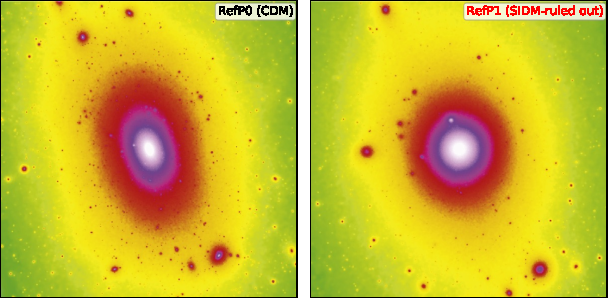
\includegraphics[width=\textwidth]{halo}}
    
    \caption{\label{fig:halo} Projected density on a \SI{270}{kpc} cube of the
    simulation of a Milky Way-like non-relativistic dark matter halo (``cold''
    dark matter, CDM). Left panel: non-interacting dark matter. Right panel:
    self-interacting dark matter (SIDM) with cross section/particle mass ratio
    \SI{10}{cm^2/g}. From \cite[21]{tulin2018}, originally from
    \cite[6]{vogelsberger2012}.}
    
\end{figure}

Where the ``Landau's arrow'' is Bayes' theorem. If the reader knows a bit about
astronomy, she may have noticed that my explanation was, to put it charitably,
qualitative. Elliptical galaxies do exist, are found in sizes smaller to larger
than the Milky Way, and possibly with low eccentricity. Furthermore,
simulations of the formation of the dark matter halo show that it actually ends
up more spherical if it \emph{does} interact, see \autoref{fig:halo}, and that
it has a rich substructure. Dark matter is expected to form aggregations of all
sizes down to the mass of the Earth \cite[1]{vogelsberger2012}.

To rule out the possibility of dark matter solar systems and planets etc.,
I~have to invoke actual measurements. In~2006 an analysis of a pair of
colliding clusters of galaxies \cite{clowe2006}, where the smaller one is named
``Bullet cluster'', showed with high confidence that the barycenters of the two
clusters have passed through, following the galaxies, while the intergalactic
gas clouds, visible in X-rays, bumped into each other. The clouds are about ten
times more massive than the galaxies, so the observed motion of the barycenters
is a strong evidence of the presence of heavy, invisible and collisionless
haloes associated to the clusters. See \autoref{fig:bullet}.

Looking at thirty such collisions, \cite{harvey2015} obtains a \SI{95}\%
confidence level upper bound on the cross section/particle mass ratio of
$\SI{0.47}{cm^2/g} = \SI{0.84}{barn/GeV}$. The limit is on the ratio, instead
of just the cross section, because the total mass is fixed by the lensing
measurement, and the mass of individual dark matter particles is unknown, and
could vary by many orders of magnitude \cite[474]{zyla2020}. This is about the
same ratio of a nucleon: cross section $\sim\SI{1}{barn}$, mass \SI{1}{GeV}.
An atom has the same mass, but cross section $10^{10}$ times higher, so
definitely dark matter is not forming anything similar to us unless we seek
very far-fetched speculations.

\begin{figure}
    
    \widecenter{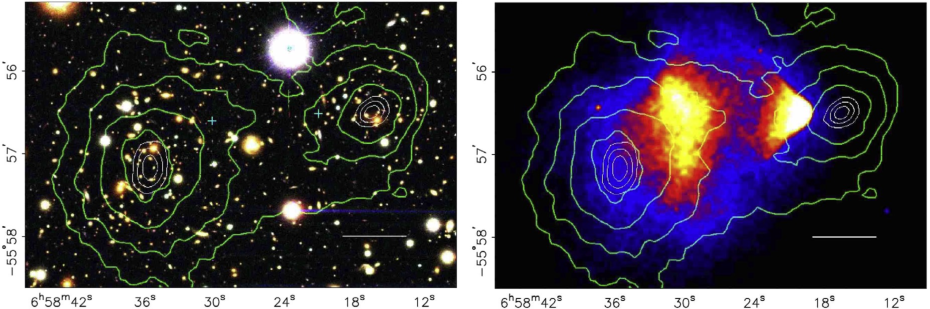
\includegraphics[width=1.3\textwidth]{bullet}}
    
    \caption{\label{fig:bullet} Left panel: photo of the Bullet cluster and its
    companion in the visible band. Right panel: the same patch of sky in
    X-rays. The contours represent the mass density obtained from gravitational
    lensing. From \cite[29]{tulin2018}, originally from \cite[3]{clowe2006}.}
    
\end{figure}

The density of dark matter in the neighborhood of the solar system can be
inferred from its effect on the motion of nearby stars, which is measured
precisely. The most recent estimate, done with the Gaia satellite data, gives
$\sim\SI1{GeV/cm^3}$ \cite{buch2019}. For comparison, the solar wind density
at the Earth orbit is some particles per~\si{cm^3}. So to have a concrete
picture in our mind we can imagine dark matter as a cloud of stable neutrons
which does not interact with ordinary matter, and with density similar to the
solar wind. The same article informs us that whether self-interacting dark
matter would form a disk is still under debate, so my improvised speculations
were not too far off the mark. Assuming that it would, they put a limit on
the fraction of self-interacting dark matter in the halo to less than~\SI1\%.

Are there any other cool things that dark matter could do, beyond parallel
worlds? I once wondered whether it would form black holes. Black holes are
thought to originate from the cores of stars and galaxies, so definitely they
involve a lot of friction to accumulate stuff in one single place until it
collapses. But a totally non-interacting matter could form a black hole through
another venue: if by coincidence a sufficient amount of fluid passes through
one point, the density can get above the critical level necessary to form a
black hole. There is no classical lower limit to the size of a black hole,
since the Schwarzschild radius is proportional to the mass.

It turns out that, given the dark matter density, this is unlikely enough to be
considered impossible. I know this because a guy at the Kavli Institute told me
so. I could not find the paper searching on the net because, when I query
``dark matter black hole'', I am swamped by a swarm of results on the
primordial black holes (PBH). They are hypothesized small black holes formed
during the big bang that could make up all or part of the dark matter. Their
mass is constrained to be less than about five solar masses, or the effect of
their individual attraction would be visible. They are a viable hypothesis for
dark matter, although under debate \cite[485]{zyla2020}.

\section{Experimental evidence}

The Bullet cluster is currently one of the most important evidences of dark
matter, since it excludes that the observed gravitational effects could be due
to a simple modification of the gravitational laws instead of the presence of
additional unseen matter. Indeed, also the very first evidence was obtained
from galaxy clusters, by \cite{zwicky1933}. He observed that in the Coma
cluster the velocity of galaxies is much higher that what would be predicted
by applying the virial theorem with the masses obtained from the expected mass
to light ratio.

As in the case of the Bullet cluster, mass excesses are also observed with
gravitational lensing. Another clear effect is the orbital speed of stars in
the galaxies. Applying Gauss' theorem, since most of the light-emitting mass
of a galaxy is concentrated in the bulge, the orbital speed should fall off
like $1/\sqrt r$. Instead, $v(r)$ rises in the bulge and then stabilizes to an
almost constant value, indicating the presence of a halo.

The other line of evidence is cosmological. The density of matter is clearly
very inhomogeneous, with aggregation at all scales. The variations of density
at the last scattering epoch correspond to the temperature anisotropies of the
cosmic microwave background (CMB), shown in \autoref{fig:planckcmb}, which are
$\sim10^{-5}$. It is predicted that the variations would increase linearly with
the scale factor of the expansion of the universe, which from the origin of the
CMB is $\approx1100$, giving a still very small factor of $10^{-2}$ nowadays.
The additional aggregation can be explained by a pre-existing matter which was
already decoupled from radiation. Moreover, the presence of this matter
directly influences the angular spectrum of the CMB, which is given by
stochastic collapse-compression-expansion cycles in the primordial plasma, and
from which it is determined that dark matter amounts to \SI{85}\% of the total
matter density of the universe. This value agrees with the gravitational
observations.

\begin{figure}
    
    \widecenter{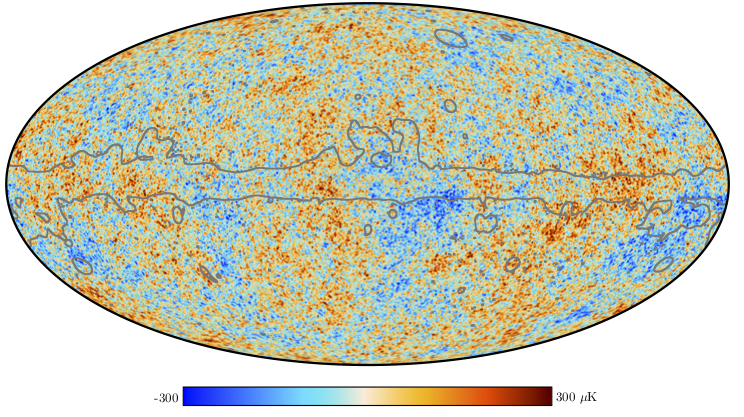
\includegraphics[width=\textwidth]{planckcmb}}
    
    \caption{\label{fig:planckcmb} Map of the variation of temperature of the
    cosmic microwave background (CMB) relative to the mean \SI{2.73}{K} and to
    the Doppler shift caused by our motion relative to the CMB. From the 2018
    Planck release \cite[fig.~6]{aghanim2020}.}
    
\end{figure}

\section{Direct detection}

All models of dark matter, apart from modified gravitational theories and
primordial black holes, postulate that dark matter is constituted by
unclassified particles. Neutrinos do behave like dark matter and account in
some part for it, but they are estimated to contribute only~\SI1\%. The limit
comes from the fact that, being relativistic (``hot'' dark matter), they would
not aggregate and solve the problem of the density variations. I have never
heard of models where dark matter is a continuous fluid.

Most of the experimental efforts are directed towards the detection of WIMPs,
``weakly interacting massive particles''. WIMP stand for a generic additional
particle in the Standard Model, which to predict the correct relic density of
dark matter after the cool down, would need to have a self-annihilation cross
section with an order of magnitude similar to the one expected for a particle
which interacts through the weak force, and a mass with an order of magnitude
around \SI{100}{GeV}.

Anyway, the point is hoping that dark matter scatters on electrons and nucleons
in the same way of a neutrino. Then, to leading order, the angular distribution
can be calculated independently of the details of the interaction. Assuming a
thermal distribution for the velocity of dark matter particles in the halo,
using the measured local mass density, and assuming a specific particle mass,
then the rate of scatterings in a target can be predicted, proportional to the
cross section. The lack of signals in a given time frame then puts an upper
limit on the cross section given the assumed mass.

\autoref{fig:sigmalimits} shows the limits obtained in this way by recent
experiments. Currently the most stringent constraints are set by experiments
hosted at Laboratori Nazionali del Gran Sasso (LNGS), DarkSide50 and Xenon1T.
Those limits are for spin-independent (SI) scattering. There are also
measurements that consider an interaction term with the spin (spin-dependent,
SD), but they are less sensible because the whole nucleus of the target atoms
counts for its overall spin, while with SI each nucleon contributes coherently.
The limits on the cross section are given per nucleon.

\marginpar{Do the limits include the uncertainties from the velocity and mass
distributions of dark matter? Are they all \SI{90}\% CL? I should read the
recent paper on statistical conventions in dark matter searches.}

From the curves it is evident that there is only a finite range of masses
probed by these searches.

The lower limit comes from the mass of the target particle. The scattering
would be detected by the recoil of the nucleus, which produces ionization and
scintillation light. If the recoil energy is too small it can not be detected,
with different thresholds depending on the detection technique, and of course
the recoil momentum goes to zero as the incoming particle mass decreases.
Considering electrons instead of nuclei, lower masses can be probed, but the
measurements are less sensitive because the radiation background of neutrons,
impacting nuclei, is kept better under control than gamma and beta rays which
impact electrons.

The upper limit is softer and comes from the fact that in this problem the mass
density of dark matter is fixed by gravitational measurements. Assuming an
higher particle mass means a proportionally lower number density, which is what
determines the rate together with the cross section, so the limits go up
linearly with the mass. In other words, the limit is the size of the target
times the exposure time.

\marginpar{There are various experiments with a clearly lower mass upper bound.
What is the cause? An upper energy threshold? Backgrounds?}

\begin{figure}
    
    \widecenter{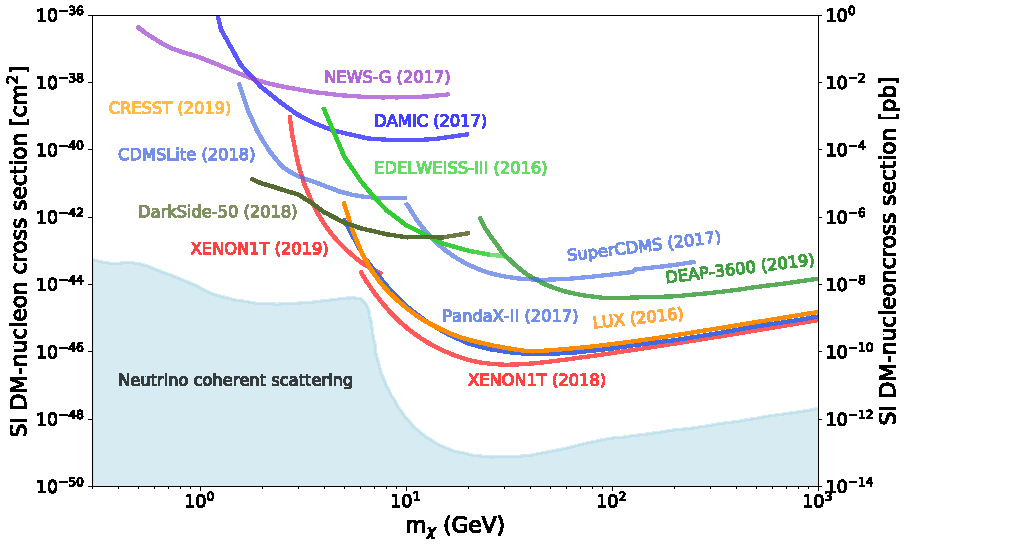
\includegraphics[width=\textwidth]{sigmalimits}}
    
    \caption{\label{fig:sigmalimits} Upper limits on the WIMP-nucleon SI
    scattering cross section, conditional on the WIMP mass. From
    \cite[fig.~27.1 p.~481]{zyla2020}.}
    
\end{figure}

The two most popular choices for the target material are liquid argon and
xenon. Being fluid, they can be purified from radioactivity to an high degree,
more than a solid scintillator. Being noble elements, ionized electrons can
drift without producing a shower or recombining, allowing to use a time
projection chamber (TPC) to reconstruct the position, which is needed to
exclude signals near the surface, where there is additional background from the
surrounding components of the detector. Of the stable noble elements, they have
the best scintillation yield, about \num{40000} photons per~\si{MeV}.

There are other dark matter models and other kinds of experimental techniques.
At the large hadron collider (LHC), dark matter is searched through missing
energy or looking for new resonances. An interesting method is discriminating
the dark matter signal from the background using the motion of the Earth
relative to the halo, which is expected to induce a seasonal variation in the
rate and directionality of the recoils. A curious proposal of this kind
considered using RNA strands to achieve high spatial and directional resolution
\cite{drukier2015}. For a complete overview on the matter, see the particle
data group \cite[sec.~27]{zyla2020}. \cite[ch.~1]{savarese2018} gives a more
detailed introduction to some topics.

    \chapter{The DarkSide experiment}
\label{ch:darkside}

% descrizione in due righe, dire che facciamo solo una breve introduzione e
%   che le cose si trovano su aalseth2018 e aalseth2019 (veto aggiornato)

% tutte le figure necessarie le dovrei trovare scorrendo aalseth2019

% descrivere la TPC
% definire S1 e S2
% descrivere il VETO

% SiPM

% DAQ

    \chapter{Data}
\label{ch:data}

We drew on two types of datasets: 1)~ data collected with the Proto0 DarkSide
prototype at CERN, and 2)~data collected with a cryogenic test stand at
Laboratori Nazionali del Gran Sasso (LNGS).

\stracka{Suona male, rifrasare ``both datasets... laser''}

Both datasets contain digital traces of photodetector modules (PDMs) output,
divided in continuous chunks of fixed length that we call ``events''.
Optionally, a pulsed laser is shone at the detector and the temporal window of
the event waveform is synchronized with the laser.

\section{Proto0}
\label{sec:dataproto0}

Proto0 is a small prototype of time projection chamber (TPC) in liquid argon
(LAr). It was built and operated in CERN building 182 in 2019, and now will be
moved and operated again in Napoli in 2021. Information is provided in the CERN
wiki page \cite{proto0}. Note that the descriptions in
\cite[sec.~4.3.2]{luzzi2020} and in the Yellow Book \cite[65]{aalseth2018}
contain outdated information relative to the status of the setup when the data
we are considering was recorded.

\stracka{Se la referenza ha una descrizione obsoleta e pertanto non
appropriata, rimuovi la referenza. \upshape Risposta: no! è proprio una
disambiguazione che serve, io quando leggo le tesi degli altri mi perdo e non
capisco cosa si riferisce a cosa. Cioè assumo che come me eventuali tesisti
futuri si debbano leggere un tot di tesi precedenti. In particolare Proto0 non
è documentato chiaramente dall'inizio alla fine da nessuna parte.}

The TPC size is $\SI{30}{cm} \times \SI{30}{cm} \times \SI{20}{cm}$. On top of
the TPC sits a photodetector unit (PDU), i.e., data transmission electronics
plus a motherboard. This specific one is dubbed ``Motherboard 2'' (MB2), and
consists of a matrix of $5\times 5$ PDMs. The silicon photomultipliers (SiPMs)
Tiles mounted in the PDMs were fabricated by Fondazione Bruno Kessler (FBK) in
2019. The tiling scheme of the motherboard is shown in \autoref{fig:pdmadcch},
while in \autoref{fig:proto0} there are some photos of the apparatus.

The PDM outputs are each sent to a channel of a CAEN V1725 analog to digital
converter (ADC) board. The ADC has \SI{16}{bit} and sampling frequency
\SI{250}{MSa/s}, downsampled in software to \SI{125}{MSa/s} to match the
specifics which will be adopted in DarkSide20k. The downsampling is simple
decimation without antialiasing, i.e., every two samples, one is discarded. The
response of the SiPMs will be described briefly in \autoref{ch:snr} and more in
detail in \autoref{ch:anal}.

Of the Proto0 data, we used only a run collected with the PDMs biased below
breakdown voltage and thus almost insensitive to light. So the waveforms
contain only electrical noise. We analyzed 1000~events, each \SI{0.5}{ms} long.
In \autoref{tab:proto0meta} we list for reference the conditions for this run.
A persistence plot of the data for Tile~53 is shown in
\autoref{fig:hist2dtile53}.

\begin{figure}
    
    \widecenter{
        \newlength\protoheight
        \setlength\protoheight{7.5cm}
        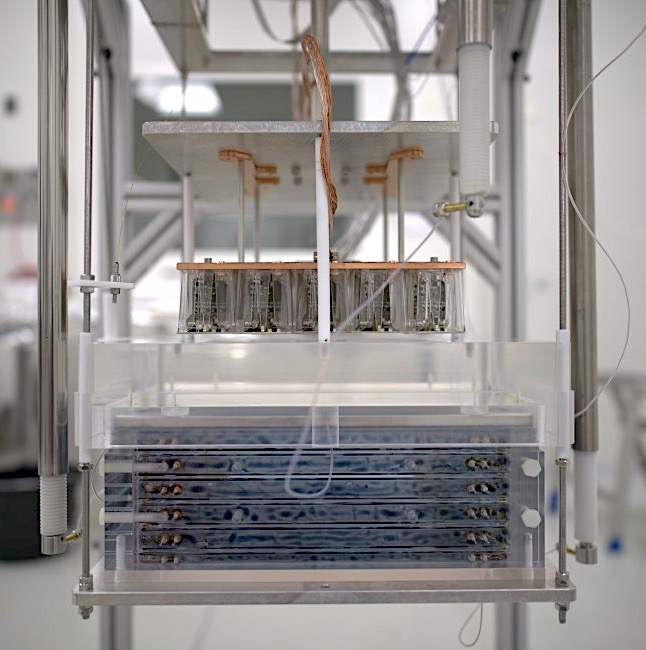
\includegraphics[height=\protoheight]{proto0-1}
        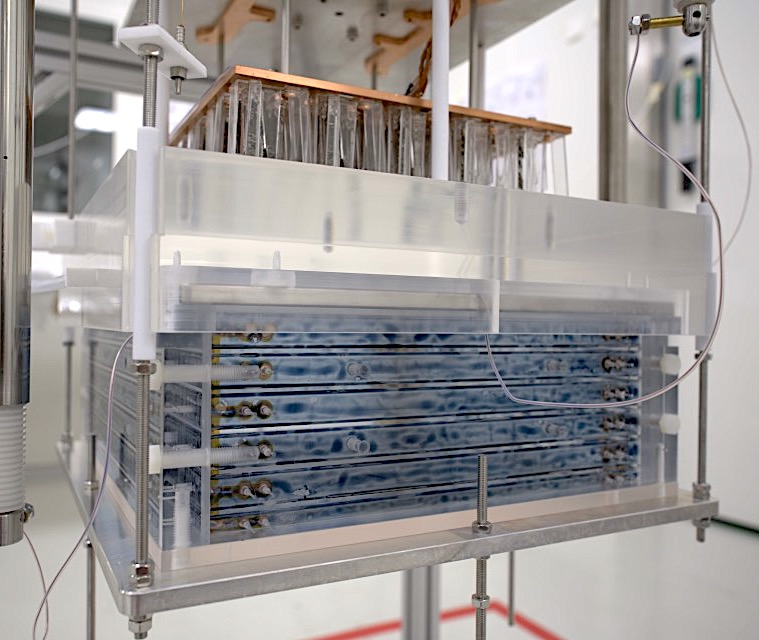
\includegraphics[height=\protoheight]{proto0-2}
    }
    
    \caption{\label{fig:proto0} The Proto0 TPC outside of the cryostat. Photos
    by Tom Thorpe (GSSI) \cite{proto0photos}. When in the cryostat, the whole
    object is completely submerged in LAr. Inside the bluish box there is a
    uniform electric field pointing top to bottom. The stripes on the sides are
    conductive and are the steps of a voltage divider, to create boundary
    conditions that keep the field uniform even near the borders. The metal
    frame visible just over the blue box, behind the semitransparent plastic,
    is the support of the grid used to create an high field region above it up
    to the anode. That region is contained in a ``gas pocket'', i.e., something
    like a cup kept upside-down underwater. The pocket is kept filled with
    gaseous argon. The copper frame on the top supports the PDMs, with their
    characteristic plastic case holding the front end board (FEB) attached
    orthogonally to the SiPMs Tile.}
    
\end{figure}

\begin{figure}
    
    \widecenter{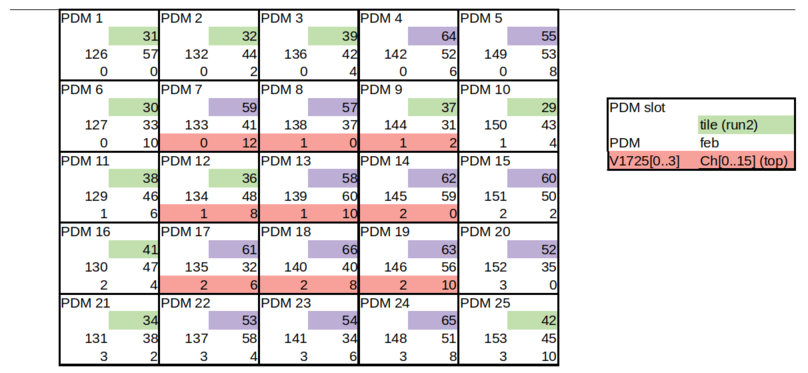
\includegraphics[width=1.2\textwidth]{PDMadcCh}}
    
    \caption{\label{fig:pdmadcch} Schematic of the motherboard installed in
    Proto0, showing the SiPM Tile identification number of each PDM and the ADC
    channels. The color of the Tile number sets apart the two set of SiPMs
    used: green ``run2'' have a higher breakdown voltage than violet ``run4'';
    being all operated at the same bias, the run2 Tiles have overvoltage
    \SI{5.5}{V} while run4 \SI{6.5}{V}. The PDMs marked in red are the inputs
    of the data trigger, which is not used in the data we consider.}

\end{figure}

% info on Proto0:
% Report_v1 Report on DAQ operation of MB1 test setup at CERN.pdf, page 1 and 2
% Kish_DS_CollabMeeting-Nov2019_Naples_Proto0 DarkSide Proto-0 activities.pdf
% Darkside_general_meeting_Napoli_Last updates on the tests and the next steps toward DS Proto 1ton.pdf, pages 12--18

\clearpage
\section{LNGS}
\label{sec:lngsdata}

\marginpar{``test stand'' è inglese o è il software della NI (labview)?}

We also used laser-run data collected at LNGS with a test stand built to
characterize individual SiPMs or Tiles, briefly described in the Yellow Book
\cite[34]{aalseth2018}, and presented in greater detail in \cite{acerbi2017}
and \cite[ch.~3]{savarese2018}. It achieves a temperature stability of
\SI{0.1}K and accuracy \SI{3}{K} in the operative range \SI{40}{K} to
\SI{300}{K}. The digitizer is a CAEN V1751. The laser light is diffused prior
to reaching the SiPM.

These datasets were collected between 2018 and 2021 by Lucia Consiglio. They
contain all the FBK Tiles used in Proto0 apart from Tile~55 (data from
2018--2019), plus other newer Tiles produced by LFoundry, Tiles~15, 21, 22,
and~23 (data from 2020--2021). The data was retrieved from the bookkeeping
directories \nolinkurl{SiPM/Tiles/FBK/NUV/MB2-LF-3x/} and
\nolinkurl{SiPM/Tiles/LFOUNDRY/pre-production-test/}. The directory name
\nolinkurl{MB2-LF-3x} stands for ``Motherboard 2, low field, triple doping''.
The data for all Tiles are collected using the same reference FEB.

The events are laser-triggered and recorded in \texttt{wav} files. Each file
contains the Tile output, and in most runs there is also the recorded laser
trigger in an additional channel, containing a square pulse marking the trigger
location, which occurs at the same place relative to the event start varying in
a \SI{23}{ns} range (see \autoref{fig:triggerhist}). Of the two-channels files
we used, the channel layout is 0:PDM, 1:trigger for FBK, swapped for LFoundry.

\stracka{As part of the preprocessing, we sort the channels in a consistent
manner (o qualcosa del genere)}

The format of the \texttt{wav} files is the following. The files are arrays of
16~bit signed integers, divided into events. Each event starts with 20 values
of metadata, followed by \num{15001} values for each channel. The ADC
resolution is 10~bit, so the values are always in the range 0 to~1023. The
sampling frequency is \SI{1}{GSa/s}.

Persistence plots of the data for tiles 15, 21, 53, 57 and~59 are shown in
\autoref{fig:hist2dtile155759}, \ref{fig:hist2dtile21}, \ref{fig:hist2dtile53},
and~\ref{fig:hist2dtile57}.

\begin{table}
    \widecenter{
        \begin{tabular}{llll}
            \toprule
            Field                 & Value        & Field                        & Value            \\
            \cmidrule(r){1-2}                    \cmidrule(l){3-4}              
            run                   & 886          & gas pocket                   & ON               \\
            date(dd-mm)           & 5-11         & laser intensity              &                  \\
            run type              & baseline run & trigger                      & external (50 Hz) \\
            Quality               & good         & trigtime (\si{\micro s})     & 100              \\
            Problem               &              & post-trigger (\si{\micro s}) & 400              \\
            Nevents (k)           &              & Time gate  (\si{\micro s})   & 500              \\
            Edrift (V/cm)         & 200          & PDM Coincidence              &                  \\
            Eextraction (kV/cm)   & 2.8          & Threshold extent (ns)        & 80               \\
            SiPM bias voltage (V) & 50           & TPC pressure (mbarg)         & >450             \\
            \bottomrule
        \end{tabular}
    }
    
    \caption{\label{tab:proto0meta} Metadata for the Proto0 baseline run~886.}
    
\end{table}

    \chapter{Signal to noise ratio of filtered photodetection signals}
\label{ch:snr}

The DarkSide20k detectors will use photodetector modules (PDMs) made up from
many silicon photomultipliers (SiPMs). For what concerns us, the output is
similar to a single SiPM output. When a photon hits the photomultiplier, the
electrical output is a sudden current spike, with a rise time on the order of
nanoseconds, which decays slowly in some microseconds.

Each SiPM is made up of many single photodiodes (called ``cells''), so when
different photons hit simultaneously different cells, the output is a signal
with an amplitude proportional to the number of photons. See
\autoref{fig:signals} for an example.

\marginpar{Bibliography for the SiPM.}

\begin{figure}
    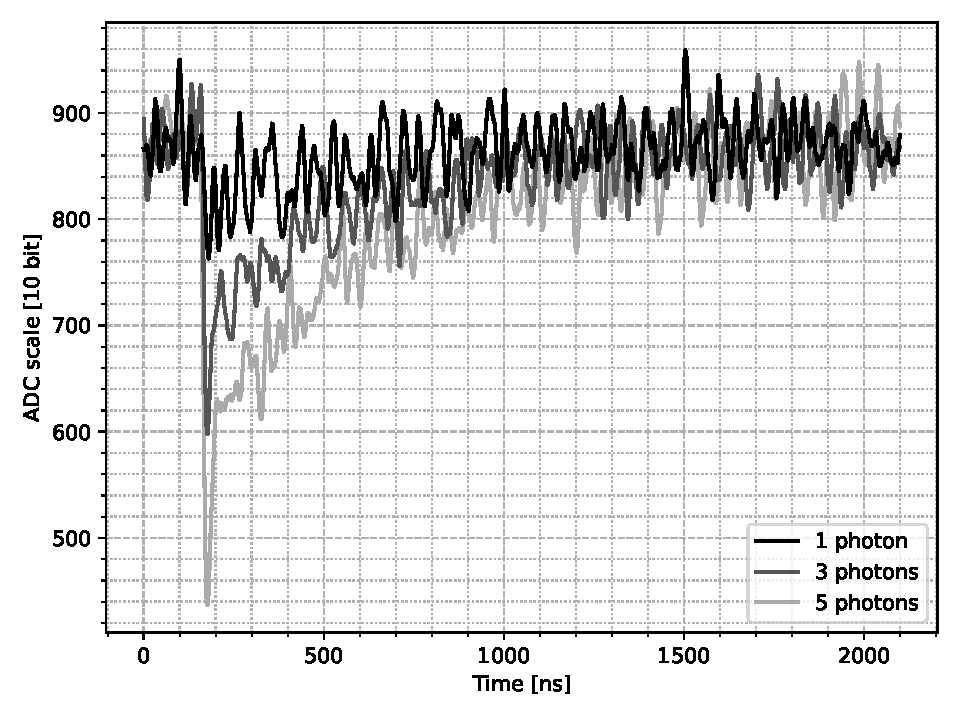
\includegraphics[width=\textwidth]{figsignals}

    \figcaption{signals}{Example PDM signals taken from the LNGS test data
    (\autoref{sec:lngsdata}). The different curves correspond to an increasing
    number of photons being detected simultaneously, with the resulting signal
    being the sum of single-photon signals. Notice that the noise amplitude is
    the same in all curves, which means that it is produced mostly outside of
    the PDM.}

\end{figure}

Our goal is to study the performance of some filters in finding and measuring
the amplitude of the signals amidst electrical noise. We'll now introduce the
dataset, list the filters tested, define a performance measure and show the
results. Finally we'll compute and comment the noise spectrum. The code for
this work is online at \url{https://bitbucket.org/Gattocrucco/sipmfilter}.

\section{Data}
\label{sec:lngsdata}

For this study we used test data taken at liquid nitrogen temperature from a
setup in the Gran Sasso National Laboratories (LNGS). A laser pulse is shot at
regular time intervals on the PDM. Both the laser trigger and the detector
output are sampled at \SI{1}{GSa/s} with a 10 bit ADC and saved separating the
data in ``events'' where each event correspond to a single laser pulse. See
\autoref{fig:lngs}.

\marginpar{Bibliography for the LNGS data. Maybe add a 2D histogram of the
data.}

\begin{figure}
    \hspace{-0.26\textwidth}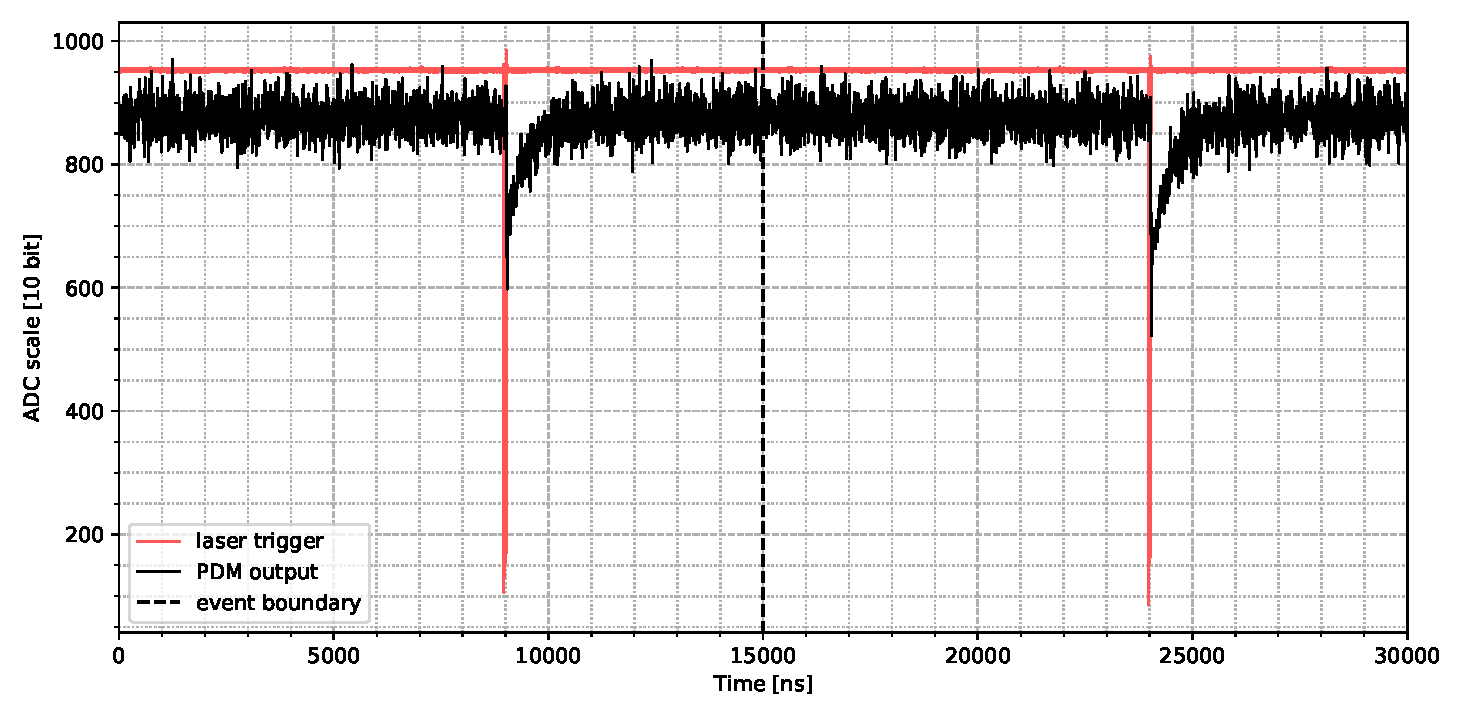
\includegraphics[width=1.52\textwidth]{figlngs}
    
    \figcaption{lngs}{A pair of events from the LNGS test data
    (\autoref{sec:lngsdata}).}

\end{figure}

We used the PDM slot 8 data, which as per \autoref{fig:pdmadcch} corresponds
to tile 57 which means the data is in the directory
\url{http://ds50tb.lngs.infn.it:2180/SiPM/Tiles/FBK/NUV/MB2-LF-3x/NUV-LF_3x_57/}. We used the file \nolinkurl{nuvhd_lf_3x_tile57_77K_64V_6VoV_1.wav}.

\marginpar{Slot 8 probably is just a Proto0 name, should mention it later. And
what are these ``tiles''?}

\begin{figure}
    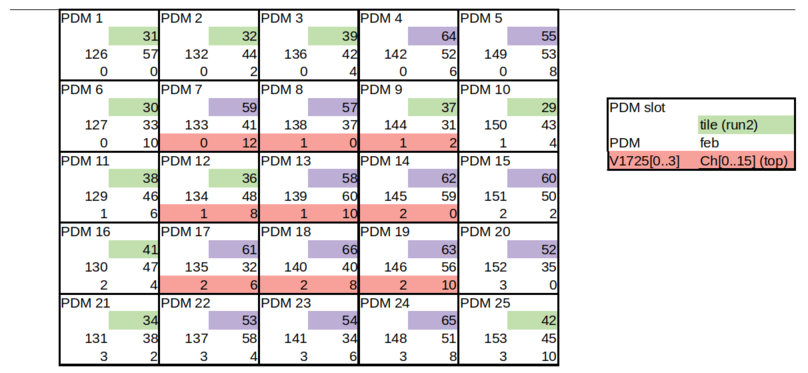
\includegraphics[width=\textwidth]{PDMadcCh}
    
    \caption{\label{fig:pdmadcch} PDM matrix of the Proto0 detector.}

\end{figure}

In the dataset there are a couple of problems. The first is that signals with
many photoelectrons saturate, however this won't trouble us since we'll need
only single photoelectron signals. The second is the presence of some spurious
signals which do not correspond to the laser pulse. I filtered these out by
putting a threshold in the part of each event \emph{before} the laser trigger,
which should be flat apart from the noise; there were 72 of them out of
\num{10005} events.

In principle a spurious signal arriving \emph{after} the ``official''
laser-induced signal matters too, however I'm ignoring them out of this logic:
spurious signals hitting earlier raise the official signal in a somewhat
uniform way with their slowly decaying tail, so the detected amplitude will
have a bias which is significant, but possibly small and as such not
identifiable. Spurious signals hitting later will add a large spike in the tail
of the official signal, so the amplitude will be noticeably higher, such that a
single photoelectron pulse gets confused as a double or higher one, and
we'll automatically ignore it as we'll consider signals detected as single.

This reasoning may fail depending on the details of filtering and the specific
relative timing of the signals, however the final most important consideration
is that I expect less than 100 spurious late pulses since there are 72 early
ones and the laser pulse is in the middle of the event, so less than \SI1\%.
See \autoref{fig:spurious} for some examples of spurious/saturated signals.

\marginpar{The afterpulse stuff I had not understood properly may change all
this.}

\begin{figure}
    \hspace{-0.26\textwidth}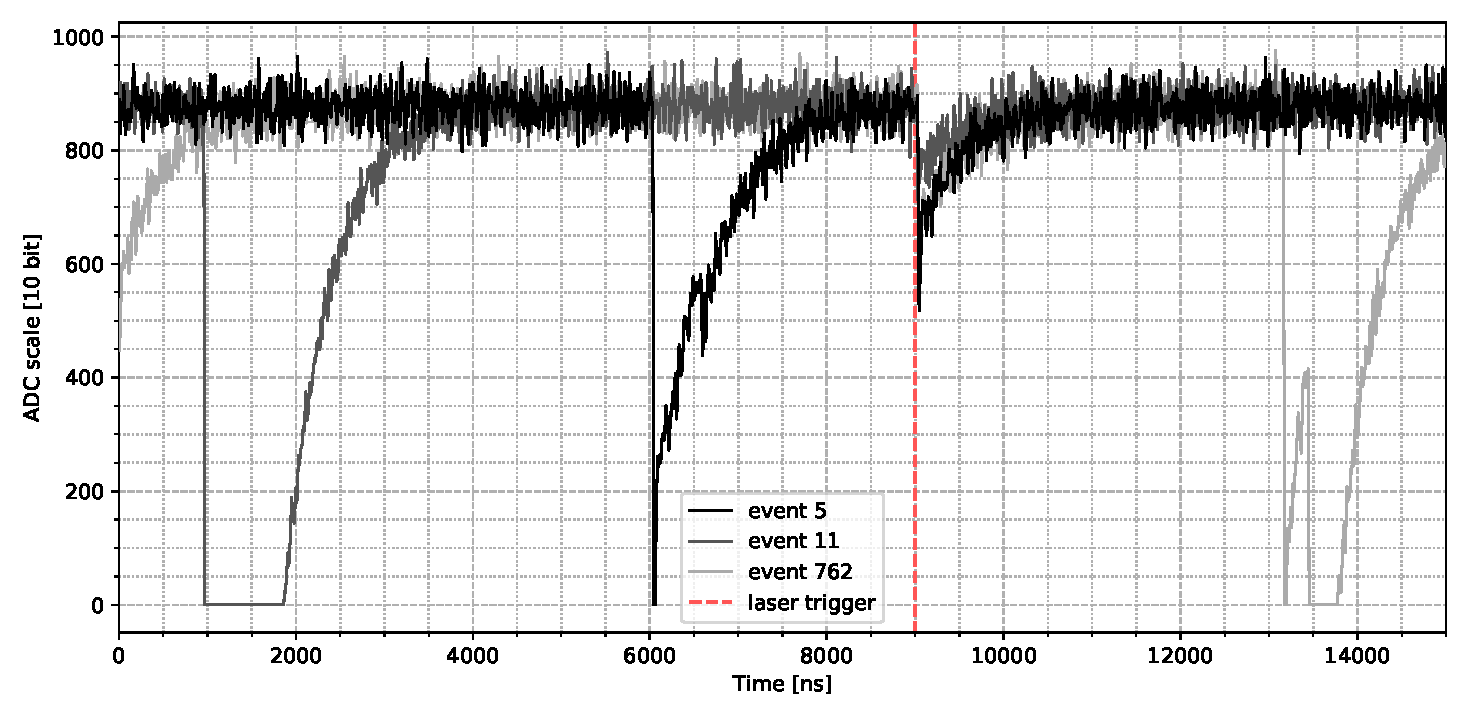
\includegraphics[width=1.53\textwidth]{figspurious}
    
    \figcaption{spurious}{Examples of spurious signals in the LNGS test data
    (\autoref{sec:lngsdata}).}

\end{figure}

\section{Filters}
\label{sec:filters}

A filter operates by converting the original sequence of ADC samples $(x_1,
x_2, \ldots)$ to a new ``filtered'' sequence $(y_1, y_2, \ldots)$. The filters
are causal, i.e. the filtered sample $y_n$ can be computed only using the
original samples up to $x_n$. This limitation is because we are interested in
using the filters online, i.e.\ produce the filter output continuously as
samples are read.

We tested three filters: the moving average, the exponential moving average or
autoregressive filter, and the cross-correlation filter.

The moving average consists in taking the average of the last $N$ samples:
%
\begin{equation}
    y_n =  \frac1N \sum_{i=1}^N x_{n-N+i}.
\end{equation}

The exponential moving average weighs past samples with an exponentially
decaying coefficient, and can be written recursively as
%
\begin{equation}
    y_n = a y_{n-1} + (1 - a) x_n, \quad a \in (0, 1).
\end{equation}
%
The scale of the exponential decay is given by
%
\begin{align}
    \tau &= -\frac1{\log a}, \\
    &\approx \frac1{1-a} \text{ for $a$ close to 1.}
\end{align}

The cross-correlation filter is the most sophisticated we considered. Let
$\mathbf h = (h_1, h_2, \ldots, h_N)$ be a \emph{template} of the signal
waveform we want to detect. This means $\mathbf h$ should ideally match the
shape of the signal waveform we want to find in the noisy data. The filter is
then the cross-correlation of $\mathbf x$ with $\mathbf h$:
%
\begin{equation}
    y_n = \sum_{i=1}^N h_i x_{n-N+i}.
\end{equation}
%
Under the assumption that the data is white noise plus a signal that perfectly
matches the template apart from amplitude, this filter is optimal in the sense
that in the filter output there will be a peak corresponding to the signal and
this peak will have the maximum possible height relative to the standard
deviation of the filtered noise.

The differences we have from the ideal case are:
%
\begin{enumerate}
    \item the shape of the signal probably changes a bit each time;
    \item the signal is not aligned always in the same way to the ADC timebase;
    \item the noise is not white.
\end{enumerate}

The variation of the actual signal shape is difficult to address directly. The
noise spectrum can be corrected by appropriately transforming $\mathbf h$, in
this case the filter is called \emph{matched filter}. Let $\mathbf s$ and
$\mathbf w$ be the signal and noise, such that the waveform to be filtered is
$\mathbf x = \mathbf s + \mathbf w$. Let $R$ be the noise covariance matrix,
i.e. $R_{ij} = \operatorname{Cov}[w_i, w_j]$. Then the template for the matched
filter is
%
\begin{equation}
    \mathbf h_\text m = R^{-1} \mathbf h.
    \label{eq:matched}    
\end{equation}

\marginpar{Explain that the matched filter is equivalent to rank~1 least
squares. As a general ref for the matched filter, use fer15.}

We tried implementing the matched filter with mixed results we will not report
in detail. We computed the noise covariance matrix on the event samples before
the signal. Since the noise is stationary, $R$ is a Toeplitz matrix, i.e. the
covariance depends only on the lag between two samples.
\autoref{fig:autocorrlngs} shows the noise covariance obtained.

\marginpar{Add the autocorrelation of the Proto0 noise to the plot.}

\begin{figure}
    \widecenter{\includempl{figautocorrlngs}}
    
    \figcaption{autocorrlngs}{Autocorrelation of the LNGS test data noise,
    computed on the part of the events before the trigger. The autocorrelation
    at lag $t$ is the correlation between a sample and another sample occurring
    a time $t$ after the first. The standard deviation of the noise is 26.7 ADC
    units.}

\end{figure}

The matched filter worked slightly better than the cross-correlation filter, as
expected, but only for $N$ sufficiently small, getting worse as $N$ increased.
This could be due to numerical accuracy problems in solving the linear system
$R$ in \autoref{eq:matched}, or in computing $R$. We didn't work on this
further since the gain is probably small.

\marginpar{Expand on the numerical issues. The uncorrected template is local,
while the template corrected for noise is less local and has large
cancellations.}

We computed the template for the cross-correlation filter by taking the median
of single photoelectron signals. We did not align the signals, we operated as
if they occurred always with the same alignment relative to the event time
window. The template obtained is shown in \autoref{fig:template}. When using
the template, we normalize it to unit sum such that the output from the
cross-correlation filter is comparable to the output from the moving averages,
i.e. if we send a flat waveform into the filter, the output has the same value
as the input.

\marginpar{Use the template from the second chapter; plot the template without
alignment, with trigger, with filtering; explain that we use 1 pe pulses to
avoid afterpulses; cite Luzzi to say it should not matter much how we compute
the template in detail.}

\marginpar{Explain that we fix the mean-like behaviour for all filters because
we have to subtract the baseline.}

Since we will try various lengths of the filter template, we have to decide how
to truncate the full template. When truncating to $N$ samples, we pick $N$
contiguous samples from the template such that their sum is the minimum
possible (recall the template is negative). Of course normalizing the template
to unit sum is done after truncation.

\begin{figure}
    \widecenter{\includempl{figtemplate}}
    
    \figcaption{template}{The template used for the cross-correlation filter.
    It is the median of unaligned single photon events from the LNGS test data.}

\end{figure}

See \autoref{fig:filters} for an example of filter output.

\begin{figure}
    \widecenter{\includempl{figfilters}}
    
    \figcaption{filters}{An event from the LNGS test data filtered with the
    three filters used. The number of averaged samples in the moving average
    filter, the scale of the autoregressive filter, and the length of the
    template of the cross-correlation filter are all 1024 samples (at
    \SI1{GSa/s}).}

\end{figure}

\section{The fingerplot}
\label{sec:fingerplot}

To measure the performance of filters, we define a signal to noise ratio (SNR)
as follows: the SNR is the ratio of the average peak filter output value for
single photon signals over the standard deviation of the filtered noise.

We could consider other similar measures, for example we could include the
standard deviation of the peak filter output value since that influences where
we should place a threshold to discriminate signals, however it is sufficient
to use any reasonable definition for the purpose of comparing different
filters. Effectively we computed the SNR without exactly respecting the
definition above, we'll see in detail.

For each event we compute the filter output at a fixed temporal delay from the
leading edge of the laser trigger pulse (see \autoref{fig:filtersample}).
Then we compute the average of the samples before the trigger pulse and take
that value as ``baseline''. We subtract the baseline from the filter output,
and finally we change the sign to obtain positive values since the signals are
negative.

\begin{figure}
    \widecenter{\includempl{figfiltersample}}
    
    \figcaption{filtersample}{Example of how a signal amplitude is computed in
    an event for the purpose of computing the SNR. The samples in the shaded
    region are averaged to compute the baseline. The filter is evaluated at a
    fixed offset (indicated by the arrow) from the leading trigger edge. The
    amplitude then is the difference between the baseline and the filter value.
    The shaded region ends 100 samples before the trigger.}

\end{figure}

We take the list of these baseline and sign corrected filter outputs and
compute an histogram. One of these histograms is shown in
\autoref{fig:fingerplot}. It is called ``fingerplot'' due to the descending
peaks reminding of fingers.

\begin{figure}
    \widecenter{\includempl{figfingerplot}}
    
    \figcaption{fingerplot}{The fingerplot for the moving average filter with
    128 samples evaluated 128 samples after the trigger.}

\end{figure}

The first peak is centered on zero and thus corresponds to cases where the
laser pulse produces no photoelectrons. Since the instant where we are
evaluating the filter output in each event is independent of the output itself
(instead of e.g.\ being determined by peak finding), this peak is the
distribution of the noise after passing through the filter.

The various other peaks correspond to an increasing number of photons. The
second peak is the distribution of the filter output at a fixed instant for
single photon signals. Assuming for the moment that the instant where we
evaluate the filter yields the highest signal response, this means that the SNR
is the mean of the second peak divided by the standard deviation of the first.

Since the peaks are often overlapping, and that we will have to repeat the
calculations for many fingerplots automatically without checking each one, we
use robust measures of location and scale instead of the average and standard
deviation. We run a peak finding algorithm on the histogram and divide the data
by putting boundaries midway between peaks, so that we assign each datapoint to
a peak. For the second peak, we take the median instead of the average. For the
first peak, we take the half symmetrized \SI{68}\% interquantile range instead
of the standard deviation, i.e.\ half the difference between the 0.84 and 0.16
quantiles. On a gaussian distribution these are equivalent to the mean and
standard deviation, however they are less sensible to messing up the tails of
the distribution, which happens since the boundaries cuts away the tails and
there is contamination from the tails of the neighbouring peaks.

\marginpar{Mention that I'm always checking that the median of the 0 pe peak
is zero within its error.}

\section{SNR versus filter length}

When determining how to compute the SNR from the fingerplot we assumed that we
were evaluating the filter output at the optimal instant. Since we do not know
it a priori, we repeat the computation for a range of values of the filter
evaluation point. A simpler solution that comes to mind is taking the minimum
(the signals are negative) of the filter output in each event, however this
would bias upward the SNR measure because the minimum can yield lower values
due to noise peaks. Instead, by fixing the point independently from the data,
the random oscillation due to noise is symmetrical and the averaging recovers
the actual amplitude of the filter output for the signal.

The resulting SNR curves are shown in \autoref{fig:snrplot}, repeated for a
range of values of the filters length parameter. For the moving average and
cross-correlation filter, the length parameter is the number of samples, $N$.
For the exponential moving average, it is the scale of the exponential decay
$\tau$.

\begin{figure}
    \widecenter{\includempl{figsnrplot}}
    
    \figcaption{snrplot}{The SNR as a function of delay from trigger (x-axis)
    and filter length (shade of gray) for the three filters.}

\end{figure}

The maximum of each curve gives the actual SNR figure we are interested in. We
expect by intuition that the width of the maximum is approximately proportional
to the temporal resolution we could achieve if we used the filter output to
locate temporally the signal. So we do another plot
(\autoref{fig:snrmaxplot}) where we show the maximum SNR value and the width
of the peak versus the filter length parameter. We measure the width as the
distance between the two points where the SNR is 1 less than its maximum value.

\marginpar{I can drop the snrmaxplot because it's already in the baseline
effect plot.}

\begin{figure}
    \widecenter{\includempl{figsnrmaxplot}}
    
    \figcaption{snrmaxplot}{Top plot: maximum SNR achieved with each filter
    (different curves) and filter length (x-axis). Bottom plot: the width of
    the maxima, computed as the length of the interval of offset from trigger
    with endpoints where the SNR is 1 less than the maximum. The
    cross-correlation filter mantains almost constant width with increasing
    SNR, while the other two filters have increasing width.}

\end{figure}

\section{Effect of the baseline computation}

In constructing the fingerplot, we subtract from the filter output value the
baseline, i.e.\ the average value of the waveform in absence of signals. We
compute the baseline for each event as the average of the samples before the
signal. More precisely, we averaged \num{8000} samples. The value obtained
varies randomly due to the noise; its standard deviation is that of the noise
divided by $\sqrt{8000}$. The maximum filter length we use is 2000, so in that
case the width of the peaks gets an additional contribution (summed in
quadrature) which is $\sqrt{2000/8000} = 1/2$ of the width we would have with a
noiseless baseline, i.e.\ the width of the first peak is $\sqrt{1 + 1/2} - 1 =
\SI{22}\%$ larger, lowering the SNR by the same percentual.

This is not just a problem of this test that can be worked around in the real
application, because how the baseline is computed is a relevant part of the
signal finding, since it requires either a fast on-digitizer algorithm
estimating it reliably or sending enough samples to subsequent stages in the
data processing chain.

To get an idea of the effect of the baseline, we repeat everything computing
the baseline with just 1000 or 200 samples. The result is in
\autoref{fig:changebs}. We see that, for example, going from 8000 to 200
baseline samples the maximum SNR drops from about 20 to about 9.

\marginpar{Explain why the SNR of the cross correlation filter drops with
increasing filter length when the baseline is short. The filter behaves like
a mean, so its peak value drops as it gets longer; the noise rms decreases too
but gets a constant contribution from the baseline variance.}

\begin{figure}
    \widecenter{\includempl{figchangebs}}
    
    \figcaption{changebs}{The same plot of \autoref{fig:snrmaxplot} repeated
    changing the number of pre-signal samples used to compute the baseline. The
    left column is the same data from \autoref{fig:snrmaxplot}, with 8000
    baseline samples. The performance decreases with a lower number of samples
    because the standard deviation of the baseline increases and the baseline
    is compared to the filtered signal amplitude to discriminate signals.}

\end{figure}

\section{Noise spectrum}
\label{sec:spectrum}

We take the region of each event before the trigger pulse, compute its
periodogram, and take the median across events for each frequency. We use the
median instead of the average in case there were spurious signals or
irregularities we missed. We do the same for data obtained with the same sensor
but when it was in the Proto0 setup, biased below breakdown voltage and sampled
at \SI{125}{MSa/s}. We thus obtain two plausible noise spectra, shown in
\autoref{fig:spectra}.

\marginpar{Source and details of the Proto0 noise data.}

\begin{figure}
    \widecenter{\includempl{figspectra}}
    
    \figcaption{spectra}{Spectrum for the PDM we used in the LNGS test data,
    both in the LNGS test data setup and in the Proto0 detector setup. While
    the LNGS data is in working conditions at liquid nitrogen temperature, the
    Proto0 data we used was taken at room temperature with sensors biased below
    breakdown voltage for the purpose of measuring noise.}

\end{figure}

We said the cross-correlation filter is optimal if the noise is white.
Actually, it is sufficient that the noise spectrum is flat in the support of
the signal spectrum, because if we filtered away frequencies outside of it, all
the signal would still be in the waveform. In \autoref{fig:templsp} we show
the power spectrum of the signal and its integral. We see that \SI{90}\% of it
is below XXX~\si{MHz}, which corresponds to an approximately flat region in the
noise spectra. This means that the cross-correlation filter is close to
optimal. \marginpar{False: most of the signal spectrum is in the rapidly
ascending part of the noise spectra.}

\begin{figure}
    \widecenter{\includempl{figtemplsp}}
    
    \figcaption{templsp}{Comparison of the spectra of signal and noise. The red
    curve shows the percentual of signal power below a given frequency. The
    signal spectrum is computed with the discrete Fourier transform of the
    cross-correlation filter template (\autoref{fig:template}) without
    windowing.}

\end{figure}

    \chapter{Temporal resolution of photon detection}

% Introduzione/sommario
%     fare un toy per la risoluzione della localizzazione

In the previous chapter we studied the performance of filters, but we did not
define an algorithm to search for signals. Neither we will do it here, we'll
skip it and measure the temporal localization precision once we know there's a
signal.

To this end, we make a simulation where each ``event'' contains only one signal
at a known position. In principle we could use the LNGS data
(section~\ref{sec:lngsdata}), but we don't know the jitter of the trigger pulse
and we may reach a temporal resolution below the sampling period, while in the
simulation we have the exact actual temporal location of signals.

The code is in the same repository of the previous chapter,
\url{https://bitbucket.org/Gattocrucco/sipmfilter/src/master/}.

% Generazione degli eventi
%     segnale
%         dati (linkare capitolo prima)
%         template (è diverso perché ho fatto la media, cambia nulla)
%         downsamplare e piazzare il template
%     rumore
%         rumore dai dati
%         downsampling
%     layout dell'evento
%         spaziature
%         definizione dell'SNR

\section{Event generation}

Each event is the sum of a signal and a noise waveform. We don't add a
baseline, so the noise has mean zero and the signals taper down to zero. The
signals are negative. We use the same scale of the LNGS data; it actually does
not matter because we are not simulating digitalization.

\subsection{Signal}
\label{sec:toysignal}

We obtain the signal waveform by averaging single photon pulses from the LNGS
data (see section~\ref{sec:lngsdata} for a description of the dataset). We do
not try to align the signals, assuming that they are aligned relative to the
beginning of each acquisition event. We take 3584 \SI1{GSa/s} samples.
Figure~\ref{fig:toytempl} shows the obtained signal template.

(A study not reported here shows that better alignment is achievable but makes
a small difference, and worse alignment means the peak of the signal is smeared
thus yielding lower performance in signal localization, and so our choice is
irrelevant at best, conservative at worst.)

\begin{figure}
    The toy template.
    \caption{}
    \label{fig:toytempl}
\end{figure}

The template is at \SI1{GSa/s}, but the simulation is at \SI{125}{MSa/s}. We
have to downsample the template and shift its temporal position continuously
instead of by $(\SI1{GHz})^{-1} = \SI1{ns}$ steps. Given the continuous
temporal position where we want to place the template, we round it by excess
and defect to the \SI{1}{ns} timebase. Then we downsample the template by
averaging samples in groups of~8, once with the groups aligned to the floor
rounded position, once with the ceiling rounded one. Finally we interpolate
linearly between the two downsampled templates. Figure~\ref{fig:interptempl}
shows a series of waveforms obtained in this way.

(Downsampling with an average is not the best antialiasing filter doable, but
it should be reasonably fine since the higher spectral part is already
suppressed in the signal template.)

\begin{figure}
    The series of interpolated templates. I think I did this in
    \verb'savetemplate.py'.
    \caption{}
    \label{fig:interptempl}
\end{figure}

\subsection{Noise}

We used three different kinds of noise: gaussian white noise; noise sampled
from the LNGS data; noise sampled from Proto0 data.

The white noise is generated in the simulation. The LNGS noise is copied from
the same data we used to make the signal template by taking the part of the
events before the signals and filtering out a few events that contained
spurious signals in that location. The Proto0 noise is copied from an
acquisition made on the same PDM when it was used in the Proto0 setup with the
SiPMs under breakdown voltage, thus inactive.

The noise obtained from data is normalized to the variance required by the
simulation. For both LNGS and Proto0 noise the data comes divided in events and
we normalized separately for each event in case the variance changed.

We downsample the noise in the same way as the signal, by averaging nearby
samples. Both noises have spectra that go down with frequency (see
section~\ref{sec:spectrum}), so this crappy antialiasing should be sufficient.
The normalization to the desired variance is done after downsampling. The order
matters because downsampling with averaging reduces the variance of the noise.
See figure~\ref{fig:noise}. The Proto0 noise data is already at \SI{125}{MSa/s}
and so did not require downsampling for most of the simulations.

\begin{figure}
    A figure similar to the one made by \verb'toy1gvs125m-plot.py' with both
    LNGS and Proto0 noise and downsampled.
    \caption{}
    \label{fig:noise}
\end{figure}

\subsection{Event layout}

Each event is the sum of a noise waveform and a shorter signal waveform. Before
the beginning of the signal there's a noise-only region long enough for the
filters to be in a stationary state when they reach the signal; in particular
its length is the highest filter length parameter used in the simulation
(\SI{2048}{ns}) plus \SI{256}{ns}.

The simulation is repeated for various signal to noise ratios (SNR). We define
the SNR as follows: the peak height relative to the baseline of the original
\SI1{GSa/s} signal template over the noise standard deviation.

Simulations with different SNR differ only in the multiplicative constant of
the noise, so we used exactly the same noise and signal arrays for each SNR to
speed up the code. This means that there's no random variation between results
obtained at different SNR (or with different filters), keep this in mind when
the smoothness of some plots would seem to suggest that the Monte Carlo error
is negligible.

Figure~\ref{fig:toyevent} shows a complete example event.

\begin{figure}
    An event. Show all filters together, plot \texttt{X}s on the minima after
    removing localization offsets at the end of \verb'Toy._run'.
    \caption{}
    \label{fig:toyevent}
\end{figure}

% Localizzazione
%     filtri
%         linkare capitolo prima
%         troncatura e downsampling template
%     ricerca del minimo
%         interpolazione
%         upsampling

\section{Temporal localization}

We run the three filters described in section~\ref{sec:filters} (moving
average, exponential moving average, cross correlation), then take the minimum
(the signals are negative) of the filtered waveform as the location of the
signal. We also take the minimum of the unfiltered waveform as baseline
comparison.

The minimum of the filter output occurs in some sense later than the signal
location, this is not a problem since the choice of the point of the signal to
be taken as reference is already arbitrary.

To make the template for the cross correlation filter, we first cut the signal
template (section~\ref{sec:toysignal}) to the required filter length, keeping
the part of the template with maximum euclidean norm, then we downsample it by
averaging nearby samples. See figure~\ref{fig:toyfilttempl}.

\begin{figure}
    The figure with the truncated templates. Was it in \verb'toytest.py'?
    \caption{}
    \label{fig:toyfilttempl}
\end{figure}

To allow for a localization eventually more precise than the sampling timebase,
we interpolate the minimum sample and its first neighbours with a parabola. We
also try upsampling the waveform to \SI{1}{GSa/s} (with sample repetition)
prior to filtering to check if it improves performance.

% Risoluzione temporale
%     istogrammi della localizzazione
%     definizione della risoluzione
%     curve di risoluzione in funzione dell'SNR
%     grafico con le curve interessanti

\subsection{Resolution}

We repeat the simulation for 1000 events for each filter, filter length
parameter, and SNR in some range, using the Proto0 noise.
Figure~\ref{fig:lochist} shows the histograms of the temporal localization for
all filters for a choice of SNR and filter length.

\begin{figure}
    Histograms of resolution. Maybe SNR=5, tau=2048 ns (very nongaussian).
    \caption{}
    \label{fig:lochist}
\end{figure}

It is evident that the distribution of localizations can be non-gaussian, so to
quantify the resolution we use, instead of the standard deviation, half the
distance between the \SI{16}\% and \SI{84}\% quantiles, which is equivalent to
a standard deviation for a gaussian, but gives a meaningful measure for the
width of the distribution even when it's highly skewed or with heavy tails.

Figure~\ref{fig:rescurve} shows the temporal resolution thus defined for each
filter, filter length, and SNR. The exponential moving average has a
consistently poor performance compared to the other filters. The
cross-correlation filter is the best one, with performance improving with
length, and at a length of 96 samples (\SI{512}{ns}) is already practically
optimal. The moving average can get close to the cross-correlation filter by
choosing appropriately the number of samples.

\begin{figure}
    Resolution curves. Use a denser SNR range.
    \caption{}
    \label{fig:rescurve}
\end{figure}

The online processing of the PDM output in the experiment will be done in two
steps: the digitizers must find the signals, then send them to the front end
processors (FEPs) for further analysis. The computational resources of the
digitizers are limited compared to the FEPs.

The exponential moving average can be surely implemented on the digitizers. The
cross-correlation with 64 samples could probably be done on the digitizers
since a similar computation was implemented in another study.

The FEPs can and should probably use the best filter, so they would run a long
cross-correlation filter. The temporal resolution matters in the FEPs but
probably not in the digitizers, in the latter case it is just a generic measure
of perfomance.

Thus out of all the temporal resolution curves the ones that matter are:
%
\begin{itemize}
    %
    \item the best we can do with the exponential moving average and moving
    average;
    %
    \item the long cross-correlation filters;
    %
    \item the 64 samples cross-correlation filter.
    %
\end{itemize}
%
We plotted these curves together in figure~\ref{fig:rescomp}, adding some
curves done with the LNGS and white noises. Note that a different noise
spectrum makes a large difference at low SNR. We also plot a curve computed
with upsampling; it does not improve significantly the performance.

\begin{figure}
    Temporal resolution comparison figure. Make it tall so that you can see the
    low resolution cc filters well together with the expmovavg. Add the
    upsampling for a good curve.
    \caption{}
    \label{fig:rescomp}
\end{figure}

% Finestra
%     come uso il filtro (condizioni al bordo, proseguimento)
%     come piazzo la finestra
%     grafici

\section{Data reduction}

We said that the digitizers must find signals in the waveform stream and send
them to the FEPs for further processing. The bandwidth of the connection
between the digitizers and the FEPs happens to be a bottleneck. Two possible
ways of reducing the amount of transmitted data are keeping only the minimum
number of samples for each signals, and reducing the sampling frequency. Both
have an effect on the temporal resolution, which we assess here.

\subsection{Waveform truncation}

We repeat the simulation, but this time we use only a fixed smaller number of
samples in each event to compute the filter output. We call this selection of
samples ``window''. On the window we run only a long cross-correlation filter
since that's what would be done on the FEPs. As past and future boundary
condition we use zero. We evaluate the filter even after the sample window end
because the window can be shorter than the filter.

While the length of the window is fixed, the placement is not fixed relative to
the true signal location. Instead we use the temporal localization with another
filter feasible on the digitizers, calibrated to have the median aligned to the
beginning of the signal template. The window then extends a given number of
samples to the left and to the right of this localization.

Figure~\ref{fig:windowevent} shows this procedure graphically for a single
event. Figure~\ref{fig:windowtempres} shows the temporal resolution versus
unfiltered SNR curves for various choices of window length, noise, and filter
used to align the window, where for reasons of computation time the latter was
computed at a fixed SNR that does not follow the value on the x-axis.

\begin{figure}
    Normal event left, windowed event right. The filter on the left is the
    filter used to center the window. Modify \verb'plot_event' and
    \verb'plot_event_window' to plot on a user-provided axis.
    
    \caption{}
    
    \label{fig:windowevent}
\end{figure}

\begin{figure}
    The four plots of resolution vs SNR for various windows from the 2020-12-10
    slides. See if it is more convenient to add options to the plotting method
    or to copy its code and modify it.
    
    \caption{}
    
    \label{fig:windowtempres}
\end{figure}

By looking at figure~\ref{fig:windowtempres}, we conclude that probably it is
sufficient to save \SI1{\micro s} of waveform to obtain practically the same
temporal resolution achievable without windowing.

What's missing in this study is that we did not try to optimize the left/right
balance of the window, and that as said above the unwindowed localization used
to align the windows is done at a mismatched SNR. The first problem can only
worsen the temporal resolution obtained, so it is conservative; the second is
conservative assuming that our choice of SNR (2.4) is lower that what we expect
in the detector.

\marginpar{Maybe with the channel summing this SNR will become realistic.}

% Altre frequenze di campionamento
%     Grafico con la risoluzione per filtro cc lungo (FEP)
%     Grafico per cose digitalizzatore (exp? cc64?)

\subsection{Downsampling}

Another way of reducing the data throughput is downsampling. In
figure~\ref{fig:tempresdowns} we show the temporal resolution achieved with a
long cross correlation filter, for white and LNGS noise, at different sampling
frequencies. We can observe that downsampling by a factor of 2 from
\SI{125}{MSa/s} to \SI{62}{MSa/s} maintains almost the same temporal
resolution, while going to \SI{31}{MSa/s} lowers it visibly.

\begin{figure}
    The figure of toy1gvs125m with also 31 MSa/s. Make it linear-linear,
    splitting it in white noise-LNGS noise.
    
    \caption{}
    
    \label{fig:tempresdowns}
\end{figure}

Since we are downsampling we also need to check if we lose signal to noise
ratio in the filter output. In figure~\ref{fig:filtsnrdowns} we plot the SNR
after filtering, defined in the same way as we did in
section~\ref{sec:fingerplot}. There's practically no difference.

\begin{figure}
    The SNR figure from toy1gvs125m, but modify toy.Toy to compute the filtered
    signal amplitude without noise such that the definition is the sensible one.
    
    \caption{}
    
    \label{fig:filtsnrdowns}
\end{figure}

    \chapter{Fake rate of photon detection}
\label{ch:rate}

In \autoref{ch:snr} we measured the signal to noise ratio after filtering.
The point of using the SNR is expressing the signal height relative to the
width of the noise distribution, because the threshold required to reject noise
with a fixed probability is proportional to that scale. So it is convenient to
express the threshold relative to the same scale, and check it is less than the
SNR so that signals are not selected away.

\marginpar{The title is misleading, since ``fake rate of \emph{photon}
detection'' would imply that DCR is included.}

Even assuming that the noise is gaussian, the probability that a random
fluctuation gets over the threshold is not given simply by computing the
survival function (i.e.\ the integral to $+\infty$) of the gaussian
distribution at the threshold.

More precisely, the probability that any given sample is above the threshold is
given by such integral. What we need, however, is the \emph{rate} of threshold
\emph{crossings}. The noise is not white, but even if it was, after applying
the filter, which combines linearly many input samples for each output sample,
the waveform is autocorrelated at least up to the length of the filter.
Intuitively, if a smooth function crosses a threshold, it takes some time to go
down before it can cross the threshold again.

Since the first stage filtering procedure that will be used in DarkSide20k is
not decided at this point, for brevity we will just see how to compute the
threshold crossing rate of the noise, called fake rate, for a specific example
filter, and check that it works. The method can then be applied to any filter
of choice.

\marginpar{Add that the model may be useful to extrapolate to very low rates
and to have a quick recipe.}

\section{Theory}

We expect the noise to be gaussian. Even if it wasn't, when filtering many
samples are linearly combined, and the sum of random variables tends to have a
gaussian distribution independently of the initial one, so we assume
gaussianity.

\subsection{From the continuous case}

We have a discrete sequence of samples. The continuous equivalent is a Gaussian
process. We can expect the discrete case to be equivalent to the continuous
case if the autocorrelation time is larger enough than the sampling step, which
should hold from the consideration above.

Also, even though the values are initially discrete too, after filtering the
possible non integer values between two consecutive integers are at least the
length of the filter (think about an average). So we take the formula for the
continuous case and adapt it.

The mean number of threshold upcrossings $r$ in the interval $(0,1)$ by a
zero-mean stationary and appropriately smooth Gaussian process is given by
\cite[81]{rasmussen2006}
%
\begin{align}
    r &= \sqrt{-\frac{k''(0)}{2\pi}} \operatorname{gauss}(u;0,\sigma) = \\
      &= \frac 1 {2\pi} \frac {\sqrt{-k''(0)}} \sigma
         \exp \left( -\frac12 (u/\sigma)^2 \right),
\end{align}
%
where $u$ is the threshold, $\sigma$ the noise standard deviation (the RMS),
$\operatorname{gauss}(x;\mu,\sigma)$ a Gaussian probability density on $x$ with
mean $\mu$ and standard deviation $\sigma$, and $k$ the autocovariance
function, i.e.\ $k(x) = \operatorname{Cov}[f(t), f(t+x)]$ for any $t$ (for
example, $k(0) = \sigma^2$), where $f(t)$ is the continuous waveform.

We have to map the second derivative of the autocovariance function to a
discrete equivalent. We first do a manipulation in the continuous realm. Since
the covariance operator is an integral, it commutes with derivation:
%
\begin{align}
    k''(x)
    &= \frac{\partial^2}{\partial x^2} \operatorname{Cov}[f(t), f(t+x)] = \\
    &= \operatorname{Cov}[f(t), f''(t+x)],
\end{align}
%
thus $k''(0) = \operatorname{Cov}[f(t), f''(t)]$. We estimate the second
derivative with a finite difference:
%
\begin{align}
    f(t \pm \Delta t)
    &= f(t) \pm f'(t) \Delta t + \frac12 f''(t) \Delta t^2 + O(\Delta t^3)
    \rightarrow \\
    \rightarrow f''(t) \Delta t^2 &=
    f(t + \Delta t) + f(t - \Delta t) - 2 f(t) + O(\Delta t^3).
\end{align}
%
Choosing $\Delta t = 1/f_s$, where $f_s$ is the sampling frequency, and calling
$y_i = f(t_0 + i\Delta t)$ the samples, we have:
\begin{align}
    k''(0) &\mapsto f_s^2 k_2, \\
    k_2 &\equiv \operatorname{Cov}[y_i, y_{i+1}+y_{i-1}-2y_i], \label{eq:k2} \\
    r &= f_s \frac 1 {2\pi} \frac {\sqrt{-k_2}} \sigma
         \exp \left( -\frac12 (u/\sigma)^2 \right).
    \label{eq:rcont}
\end{align}
%
The reader can check that discretizing directly $k''(0)$ yields the same result.

The covariance in \autoref{eq:k2} can be estimated with the sample
covariance on a filtered waveform array~$\mathbf y$.

\subsection{Direct discrete derivation}

Since the formula we derived is approximate, as a cross check we derive another
approximate one following a different path.

A threshold crossing happens when a sample is below the threshold and the next
one is above: $y_i \leq u$, $y_{i+1} > u$. Fix $i=0$ and let $p(y_0,y_1)$ be the
joint distribution of the two samples. The probability of crossing at any given
point then is
%
\begin{equation}
    P =
    \int_{-\infty}^u \mathrm d y_0\,
    \int_u^\infty \mathrm d y_1\,
    p(y_0, y_1).
    \label{eq:crossingprob}
\end{equation}

In general we can not obtain the crossing rate just by multiplying $P$ by the
sampling frequency because of correlations. However in practice we are
interested in low crossing rates, on the order of~\SI{10}{cps}, to be compared
to the sampling frequency~\SI{125}{MSa/s}. If the typical time between
crossings is much longer than the autocorrelation time, then we can ignore
correlations. Thus the crossing rate is $r = f_s P$.

\marginpar{Correction: we are interested in fake rates \emph{less} than 10,
to be compared with the filter length \SI2{\micro s}.}

The integrand in \autoref{eq:crossingprob} is a bivariate gaussian
distribution, which explicitly is
%
\begin{equation}
    p(y_0,y_1) =
    \frac 1 {2\pi \sqrt{\sigma^4 - c^2}}
    \exp \left(
    \frac 1 2
    \begin{pmatrix}
        y_0 & y_1
    \end{pmatrix}
    \begin{pmatrix}
        \sigma^2 & c \\
        c & \sigma^2
    \end{pmatrix}^{-1}
    \begin{pmatrix}
        y_0 \\ y_1
    \end{pmatrix}
    \right),
\end{equation}
%
where $c = \operatorname{Cov}[y_0, y_1]$.

We don't know how to the integral analytically, so we break down the joint
distribution as $p(y_0,y_1) = p(y_1|y_0) p(y_0)$ and discretize the integral
over~$y_0$:
%
\begin{align}
    p(y_0) &= \operatorname{gauss}(y_0; 0, \sigma), \\
    p(y_1|y_0) &= \frac {p(y_0, y_1)} {p(y_0)}
    = \operatorname{gauss} \left(
        y_1; \frac c {\sigma^2} y_0, \sqrt{\sigma^2 - \frac {c^2} {\sigma^2}}
    \right), \\
    P &\approx
    \sum_{k=0}^{N-1} \Delta u\, p(y_0(k,u,\Delta u))
    \int_u^\infty \mathrm d y_1\, p(y_1|y_0(k,u,\Delta u)), \label{eq:rdisc} \\
    y_0(k,u,\Delta u) &\equiv u - k \Delta u.
\end{align}

The integral on $y_1$ can be computed using the error function. $\Delta u$
should be chosen small compared to $\sigma$, while $N$ large relative to
$\sigma / \Delta u$.

In \autoref{fig:crossingprob} we compare formula~\eqref{eq:rcont} (with $f_s
= 1$) with $P$ and with the Gaussian survival function. To make the comparison
we have to use a $k_2$ that matches $c$:
%
\begin{align}
    k_2 &= \operatorname{Cov}[y_i, y_{i+1}+y_{i-1}-2y_i] = \notag \\
    &= \operatorname{Cov}[y_i,y_{i+1}]
    + \operatorname{Cov}[y_i,y_{i-1}]
    - 2 \operatorname{Cov}[y_i,y_i] = \notag \\
    &= 2 (c - \sigma^2). \label{eq:c2k2}
\end{align}
%
We use $\sigma=1$, $c = \SI{99}\%$, $\Delta u = 1/100$, $N=500$ (we decreased
$\Delta u$ until convergence). We see that our derivation and the formula
for Gaussian processes agree very well, while differing visibly from the
survival function. We will henceforth use the continuous formula for its
simplicity.

\marginpar{Use the formula for white noise with \SI{40}{MHz} low-pass from the
Yellow book or Savarese and put it in \autoref{fig:crossingprob}. The
\SI{40}{MHz} is from Savarese pag.~98 right after formula~5.4.}

\begin{figure}
    
    \hspace{0.00\textwidth}
    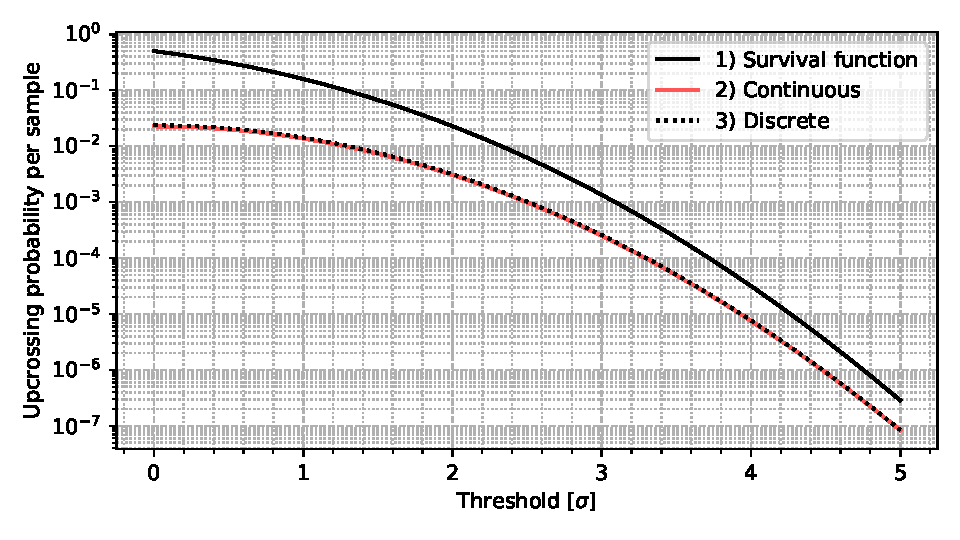
\includegraphics[width=1.00\textwidth]{figcrossingprob}

    \figcaption{crossingprob}{The threshold upcrossing rate expressed as
    per-sample crossing probability (i.e.\ the rate if the sampling frequency
    is~1) for an autocorrelated Gaussian waveform, estimated using three
    formulae: 1) the probability for a single sample to be higher than the
    threshold, 2) a formula for continuous processes (\autoref{eq:rcont}),
    3) an approximation of the discrete case (\autoref{eq:rdisc}).}
    
\end{figure}

\subsection{Dead time}

The part of the data acquisition system (DAQ) that will look for threshold
crossings are the digitizers. A digitizer can not do complicated processing, so
when the threshold is crossed, a fixed slice of waveform is sent to the front
end processing (FEP) for further analysis (identify multiple signals, locate
them precisely, use a better filter, etc.). So we are not interested in
threshold crossings that happen close to a previous crossing.

This means that we have a dead time $T$. We arbitrarily decide to use a
non-restartable dead time, i.e.\ a crossing that happens within $T$ of a
previous one is ignored only if the latter has not been ignored itself.

Assuming that the crossings are a Poisson process, the formula to correct a
rate $R$ for the effect of the dead time is \cite[120]{knoll2010}:
%
\begin{equation}
    R \mapsto \frac R {1 + RT}. \label{eq:deadrate}
\end{equation}

The crossings of a Gaussian process are not in general a Poisson process. We
just need one counterexample to show this. Consider the process with
autocovariance function $k(x)=\cos(x)$. This is positive definite because it is
a linear combination of external products: $\cos(x-y) = \cos x \cos y + \sin x
\sin y$. Since $\cos$ is orthogonal to $\sin$, they are the eigenfunctions, so
a realization of the process is a random linear combination of harmonic
functions, which means that it is a shifted cosine, so the crossings are
exactly periodic.

However, in practice we expect that there will just be a ``repulsion'' or
``attraction'' of crossings within the scale of the autocorrelation time, so
for low crossing rate the formula should work.

\section{Test}

We want to test formula~\eqref{eq:rcont} on actual electrical noise.

\subsection{Data}

We will use the Proto0 run 886, a baseline acquisition. Tiles 53, 57 and 59
(used in Proto0) will be also studied with LNGS data. Tile~15 just with LNGS.
The LNGS data files are:
%
\begin{verbatim}
FBK/NUV/MB2-LF-3x/NUV-LF_3x_53/nuvhd_lf_3x_tile53_77K_64V_6VoV_1.wav
FBK/NUV/MB2-LF-3x/NUV-LF_3x_53/nuvhd_lf_3x_tile53_77K_66V_7VoV_1.wav
FBK/NUV/MB2-LF-3x/NUV-LF_3x_57/nuvhd_lf_3x_tile57_77K_64V_6VoV_1.wav
FBK/NUV/MB2-LF-3x/NUV-LF_3x_59/nuvhd_lf_3x_tile59_77K_64V_6VoV_1.wav
LFOUNDRY/pre-production-test/TILE_15/LF_TILE15_77K_55V_0VoV_1.wav
LFOUNDRY/pre-production-test/TILE_15/LF_TILE15_77K_59V_2VoV_1.wav
LFOUNDRY/pre-production-test/TILE_15/LF_TILE15_77K_63V_4VoV_1.wav
LFOUNDRY/pre-production-test/TILE_15/LF_TILE15_77K_67V_6VoV_1.wav
LFOUNDRY/pre-production-test/TILE_15/LF_TILE15_77K_71V_8VoV_1.wav
LFOUNDRY/pre-production-test/TILE_15/LF_TILE15_77K_73V_9VoV_1.wav
\end{verbatim}

\marginpar{Expand and adapt this paragraph after chapter 3 is done.}

The Proto0 data is without signals so we use it as it is. For the LNGS data
we take the pre-trigger part of the events, and ignore events where any
pre-trigger sample is less than~750 (860 for tile~15).

We plot the time-value histogram of the data for tile 53 in Proto0 and LNGS
(\autoref{fig:hist2dtile53}), for tile 15 at maximum overvoltage, and for
tiles 57 and 59 (\autoref{fig:hist2dtile155759}).

\marginpar{No need for more explanations of the time-value histograms since
there will be some of them in chapter 3.}

\marginpar{Move the histograms to the end of the chapter.}

\begin{figure}
    
    \mbox{
    \hspace{-0.20\textwidth}
    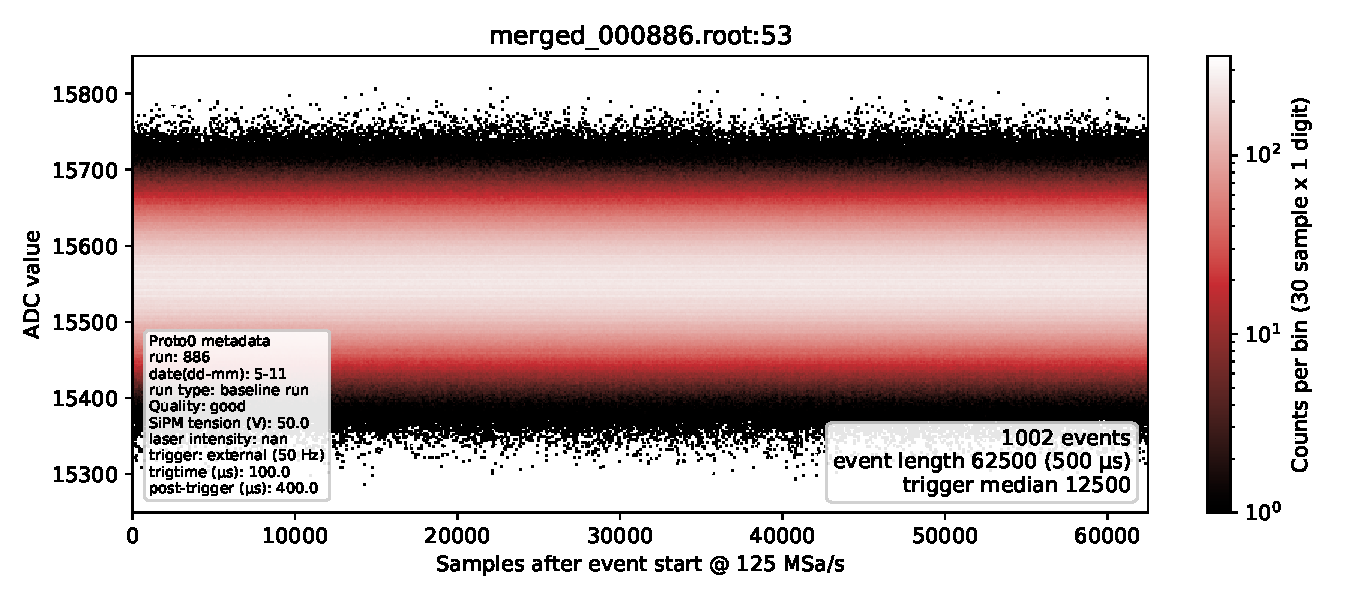
\includegraphics[width=1.41\textwidth]{fighist2dtile53-0}
    }
    \mbox{
    \hspace{-0.20\textwidth}
    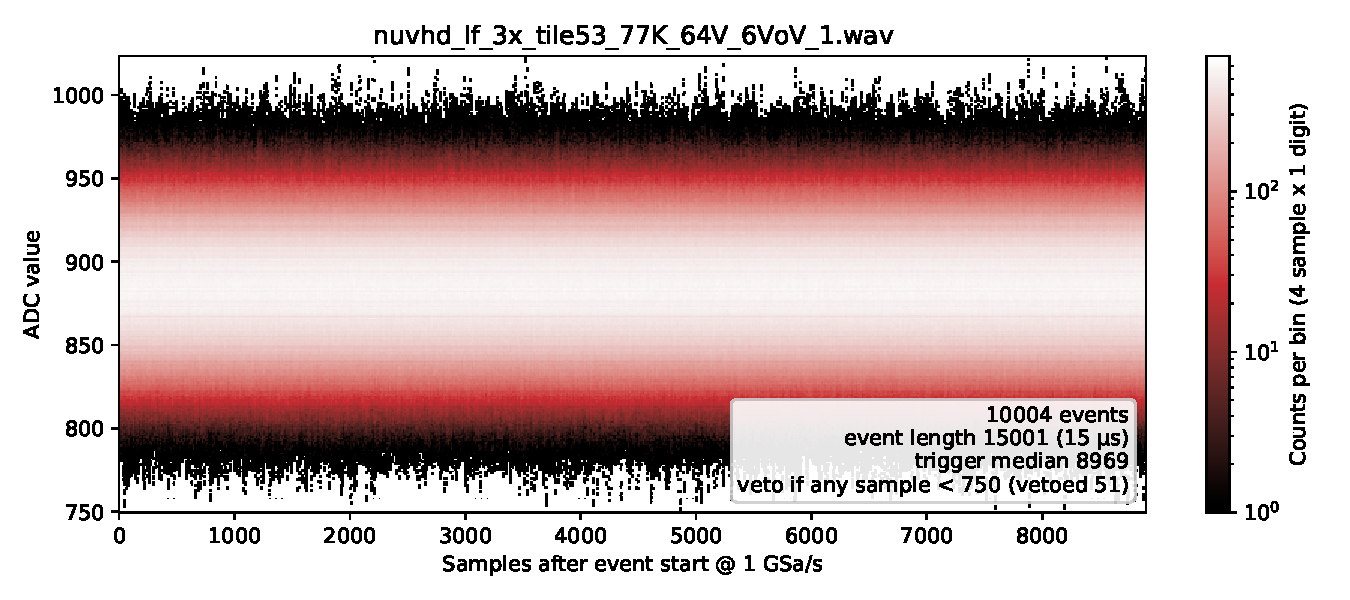
\includegraphics[width=1.41\textwidth]{fighist2dtile53-1}
    }
    \mbox{
    \hspace{-0.20\textwidth}
    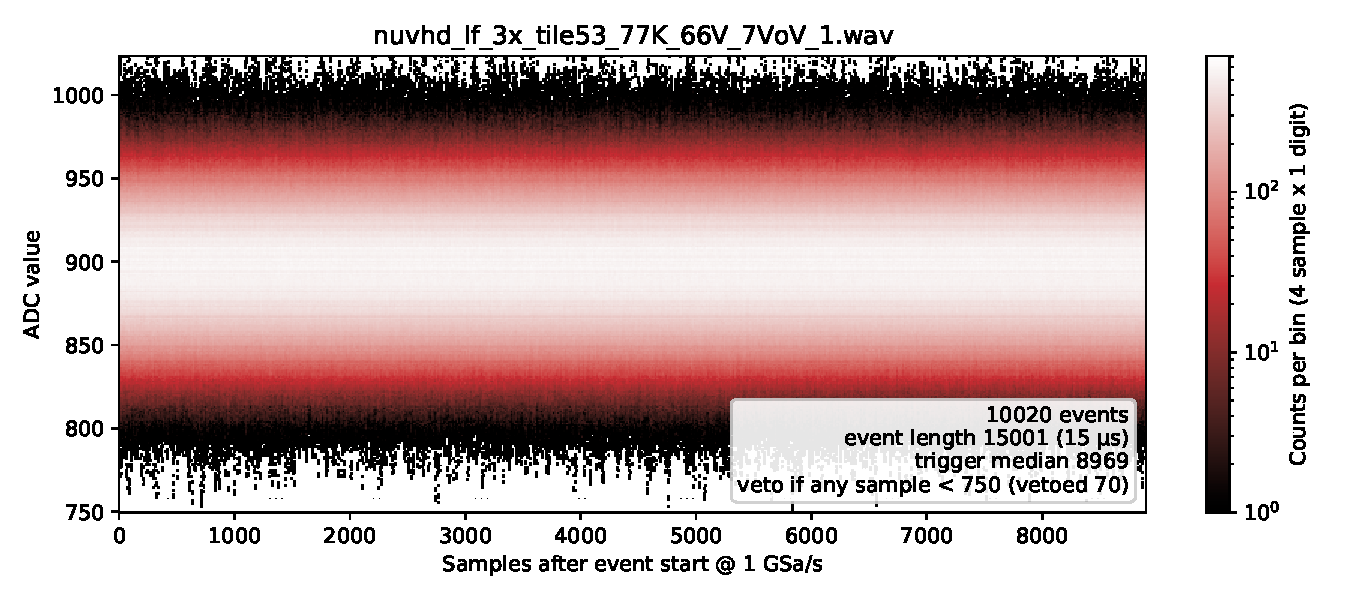
\includegraphics[width=1.41\textwidth]{fighist2dtile53-2}
    }
    
    \figcaption{hist2dtile53}{Time-value histograms of tile 53 noise in Proto0
    with a baseline acquisition, and in LNGS pre-trigger at overvoltage \SI6V
    and \SI7V.}
    
\end{figure}

\begin{figure}
    
    \mbox{
    \hspace{-0.20\textwidth}
    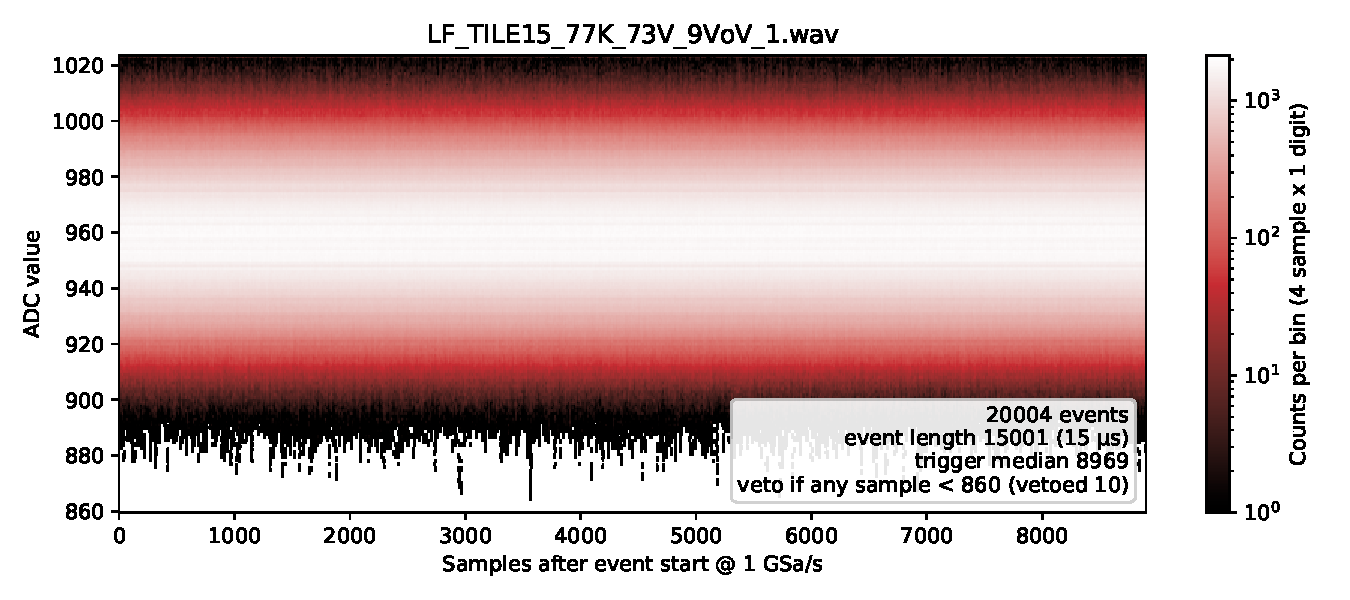
\includegraphics[width=1.41\textwidth]{fighist2dtile155759-0}
    }
    \mbox{
    \hspace{-0.20\textwidth}
    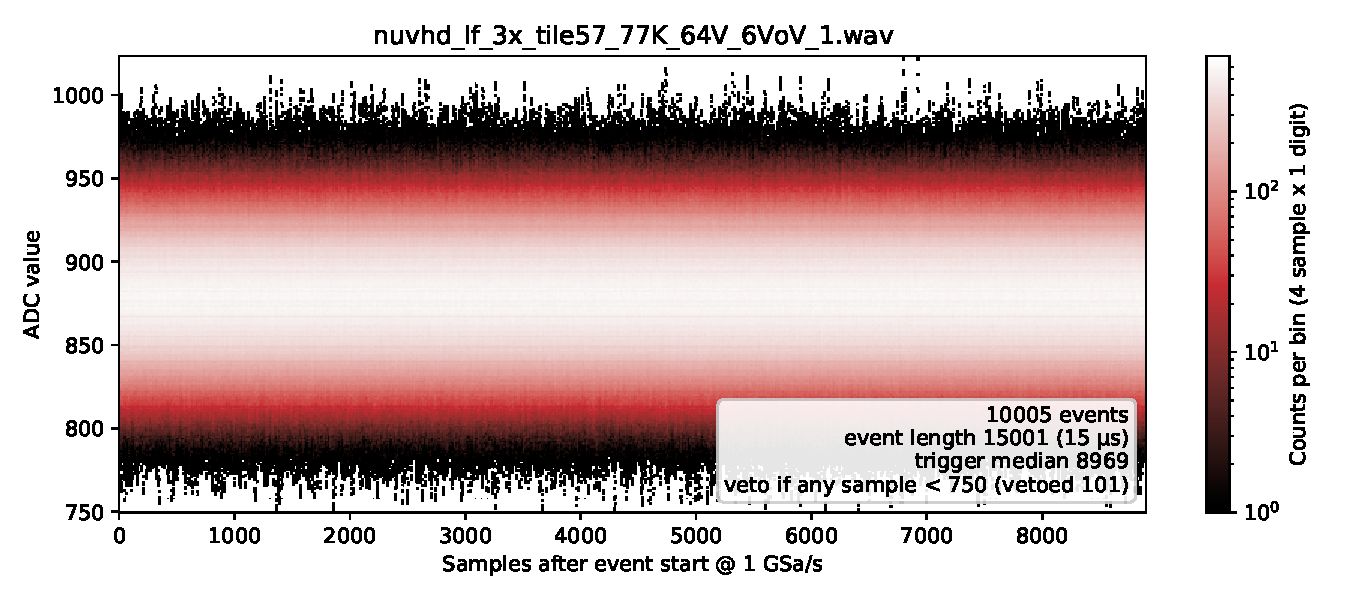
\includegraphics[width=1.41\textwidth]{fighist2dtile155759-1}
    }
    \mbox{
    \hspace{-0.20\textwidth}
    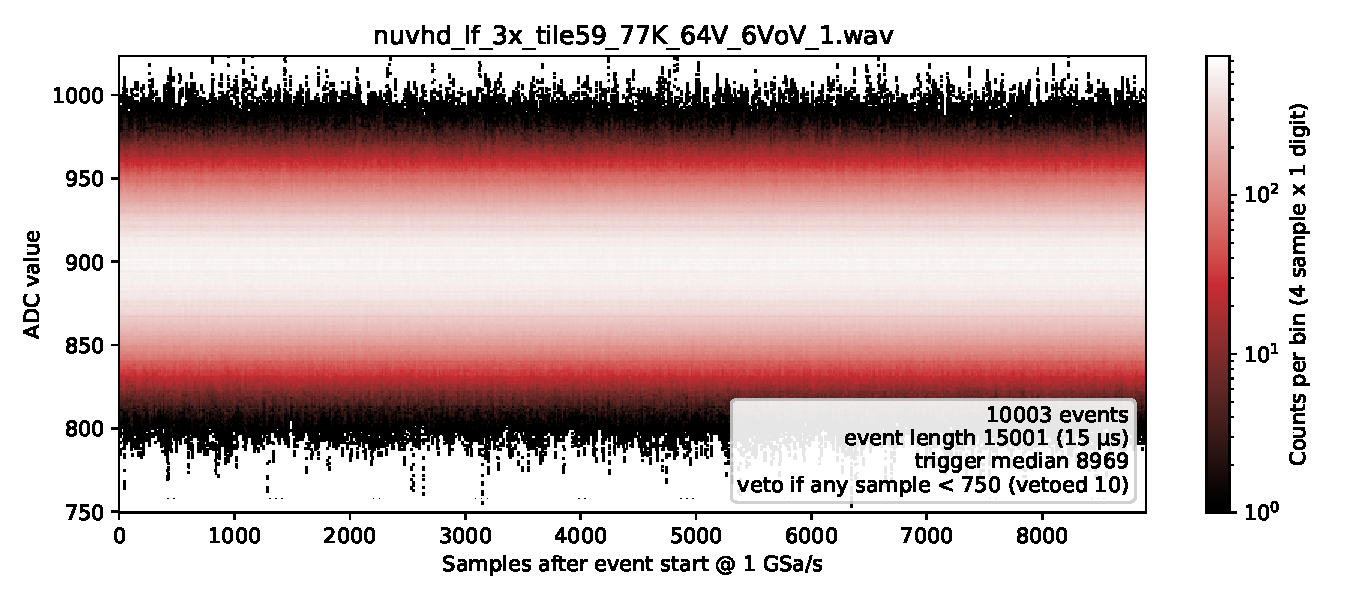
\includegraphics[width=1.41\textwidth]{fighist2dtile155759-2}
    }

    \figcaption{hist2dtile155759}{Time-value histograms of tiles 15, 57 and 59
    noise in LNGS data.}
    
\end{figure}

\subsection{Filter}

We filter using a \SI1{\micro s} moving average with \SI1{\micro s} of baseline
and \SI1{\micro s} of dead time, without delay between the baseline and the
signal averages. In \autoref{fig:sqfilt} we show an example filtered
waveform and the filter shape.

\begin{figure}

    \hspace{-0.20\textwidth}
    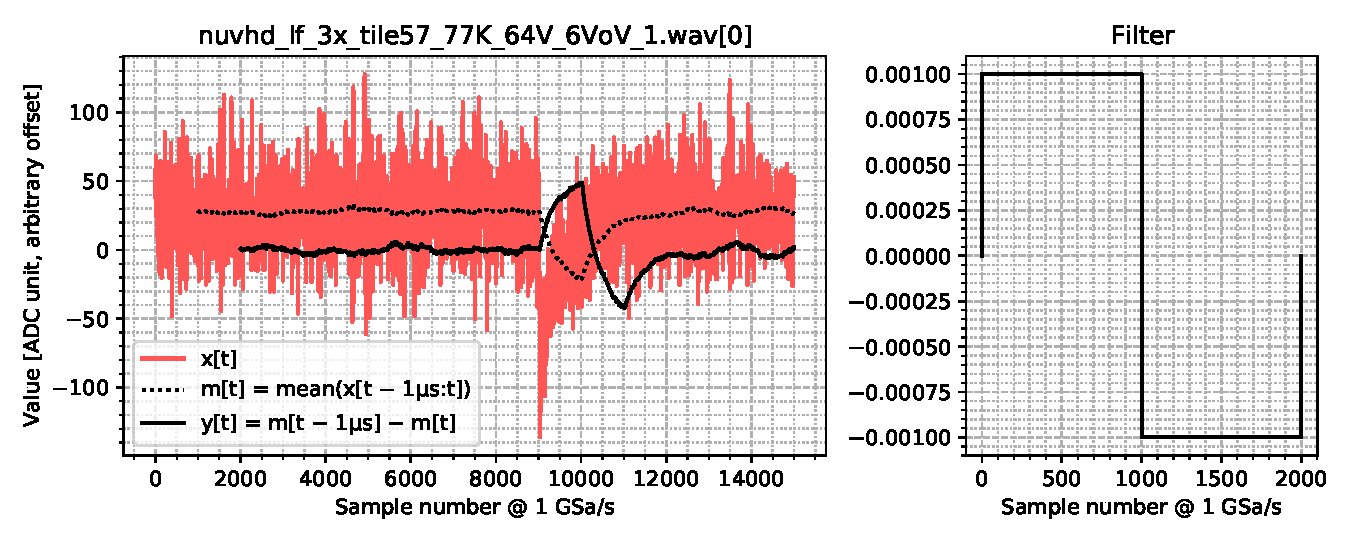
\includegraphics[width=1.41\textwidth]{figsqfilt}

    \figcaption{sqfilt}{A filtered waveform. The computation is split into a
    moving average $m$ (dotted line) and its finite difference $y$ (solid black
    line). The right plot shows the overall filter shape. (We use an event with
    a signal just to see how the filter behaves, the analysis is done on noise
    only.)}

\end{figure}

From Chapters~\ref{ch:snr} and~\ref{ch:timeres} we know this is not the optimal
filter by SNR neither by temporal resolution. However since we don't know which
filter will be used it is appropriate to make a conservative choice.

Since on LNGS data the events are short compared to the filter length
(\SI9{\micro s} vs. \SI2{\micro s}), we need to take into account boundary
effects. The output length of the filtered waveform is $(\text{initial length})
- \SI2{\micro s} + \SI1{sample}$; to compute the rate we have to divide by this
quantity instead of the initial waveform length.

The dead time does not play nicely with borders, because a hypothetical unseen
crossing within \SI1{\micro s} before the event start could kill a crossing in
the event. Moreover, at low thresholds, the first crossing will happen
almost immediately, and again immediately after the dead time ends, thus the
number of crossings per event is quantized.

A complete solution to these problems would be to avoid counting the crossings
which happen within \SI1{\micro s} after the event start (although they are
detected and do project a dead time on the following ones), and in the
remaining region further select a subregion which is \SI1{\micro s} shorter but
has a uniformly random starting position.

However we care only about low rates, and at low rate the dead time boundary
effects are negligible, so we will keep the whole filtered region.

\subsection{Algorithm}

The simplest way to count the threshold crossings as a function of the
threshold is to repeat the calculation varying the threshold. The computational
complexity is $O(nN)$ where $n$ is the number of thresholds and $N$ the number
of samples.

To produce a smooth curve (large $n$) we use instead a reverse histogram. We
choose an evenly spaced range of thresholds. For each pair of consecutive
samples, if the second sample is higher than the first, we determine the
subrange of thresholds that falls between the samples, and increment their
counts. To apply the dead time, we keep a per-threshold last occurence time.

Since the range of thresholds is evenly spaced, the subrange can be found
arithmetically, so the complexity is just $O(N)$, it does not depend on the
number of thresholds.

\subsection{Results}

In \autoref{fig:fakerate1} we compare the measured threshold crossings with
the continuous-derived formula~\eqref{eq:rcont} for a single tile over the
entire threshold range. The coefficients $\sigma$ and $k_2$ for the formula are
computed on each filtered event and then averaged. Finally, the dead time is
accounted for with~\eqref{eq:deadrate}. For the data, the conversion from count
to rate is done dividing by the length of the filtered waveform (so \SI2{\micro
s} less than the initial length per event).

The agreement is decent at low and high rates, less so in an intermediate
region. The agreement at high rate is probably a sort of saturation due to dead
time, since the maximum rate allowed by dead time is $1/(\SI1{\micro s}) =
\SI1{Mcps}$. Keep into account that the scale is logarithmic, so even where the
lines are closer they still differ by a factor~1.3, while the Poisson error is
approx.~\SI3\% since the count is~1000.

\begin{figure}
    
    \hspace{-0.11\textwidth}
    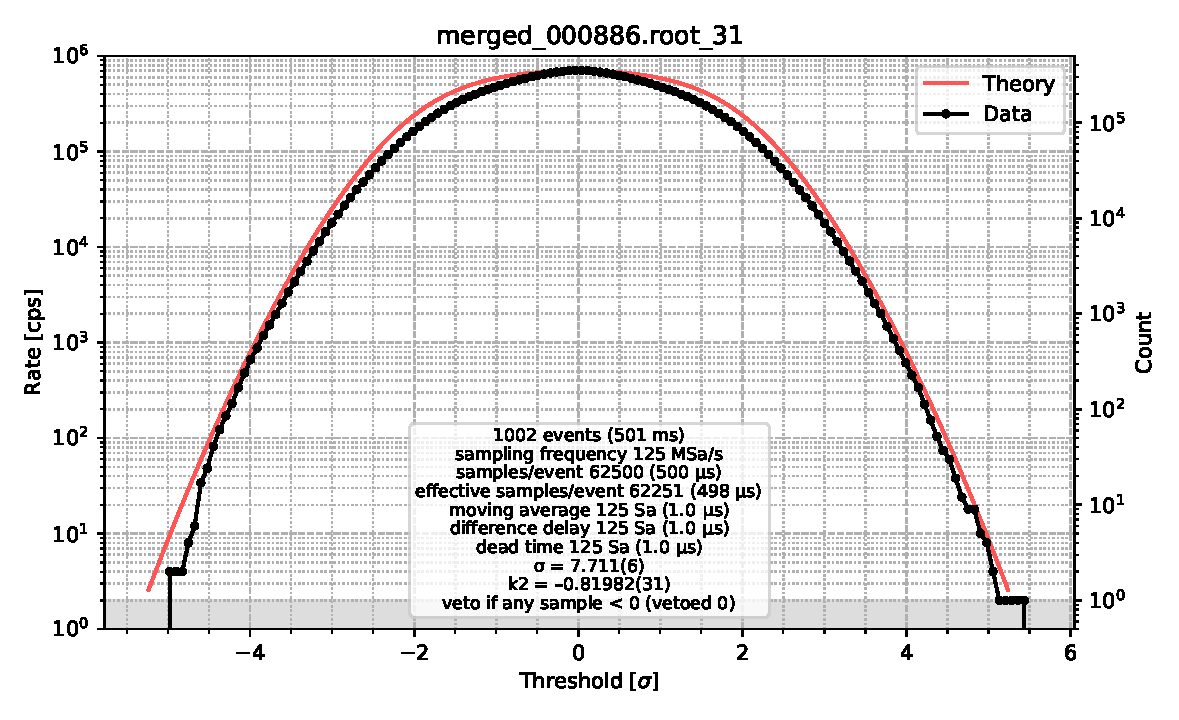
\includegraphics[width=1.23\textwidth]{figfakerate1}

    \figcaption{fakerate1}{Measured and predicted fake rate for tile~31 in
    Proto0 with a noise-only acquisition. The right scale shows the actual
    count of threshold crossings for the data, with a gray band marking one
    crossing.}
    
\end{figure}

\marginpar{Add reference to the formula in \autoref{fig:fakerate1}.}

In \autoref{fig:fakerate} we show the same comparison together for all
datasets, divided in three groups (tile~15 LNGS data, Proto0 data, LNGS other
tiles). The parameters for the formula, and the rates at threshold~$4\,\sigma$,
are listed in \autoref{tab:fakerate}.

In the second group above some threshold the measured rate stops decreasing and
remains constant at approximately 10 counts. This is probably due to pulses
which our very simple veto can not filter away, we guess 1 pe dark/random
pulses.

In \autoref{fig:fakerate} we highlight the measured rates for tile~53
because they are evident outliers. The rate remains higher than the theory
predicts and than the other tiles as the threshold increases. This is visibile
in Proto0, and in LNGS at \SI6{VoV}, but not at \SI7{VoV}.

Analogously, from \autoref{tab:fakerate} we see that the quantity $f_s
\sqrt{-k_2}/(2\pi\sigma)$ that multiplies the exponential in~\eqref{eq:rcont}
is different from the others for tile~53, in the same cases as the data, but
with the opposite trend. This variation seems to depend only on an increase in
$\sigma$ and not on $k_2$.

Even though it's weird that this problem disappears at \SI7{VoV}, it can't be a
coincidence that it arises for the same tile in different setups, showing up
both as an increased noise RMS and an higher threshold crossing rate, so it
must be some property of the tile itself.

Comparing the 2D histograms for tile~53 (\autoref{fig:hist2dtile53}) to the
others (\autoref{fig:hist2dtile155759}) there is no apparent difference.
Three possible explanations come to mind: 1) a violation of Gaussianity, 2)
stray pulses, 3) electrical noise.

Regarding Gaussianity, we checked the distribution of the samples before
filtering and it agrees very well with a Gaussian. If they are stray pulses,
they do not have the same height, otherwise they would show up as a flat rate
curve. It could be electrical noise with a frequency of approx.~$1/(\SI2{\micro
s}) = \SI{500}{kHz}$, since our filter would be very good at picking that up.

\marginpar{Looking at the spectrum it is evident that there's a very low
frequency component ($<\SI{10}{kHZ} = 1/(\SI{100}{\micro s})$) absent in other
tiles. Maybe they are sudden changes of baseline? I should look at events where
crossings with high threshold happen.}

\begin{table}
    
    \hspace{-0.17\textwidth}
    \begin{tabular}{
        c
        S[table-format=2]
        S[table-format=>1]
        S[table-format=3]
        S[table-format=2.1]
        S[table-format=+1.4]
        S[table-format=2.3]
        S[table-format=1.1]
        *2S[table-format=1.2]
    }
        \toprule
        \multicolumn3c{Data}
        &
        &
        &
        &
        &
        & \multicolumn2c{Rate @ $4\,\sigma$} \\
        \cmidrule(r){1-3} \cmidrule(r){9-10}
        
        Setup
        & {Tile}
        & {Overvoltage}
        & {$T$}
        & {$\sigma$}
        & {$k_2$}
        & {$\operatorname{Std}[\bar{k_2}]\sqrt T$}
        & {$f_s \sqrt{-k_2}/(2\pi\sigma)$}
        & {Theory}
        & {Data} \\
        
        &
        & {[\si{V}]}
        & {[\si{ms}]}
        & {[\si{u}]}
        & {[\si{u^2}]}
        & {[\si{u^2 ns^{1/2}}]}
        & {[\si{Mcps}]}
        & {[\si{kcps}]}
        & {[\si{kcps}]} \\
        \midrule
        
  LNGS & 15 &  0 & 138 &  1.6 & -0.0017 & 0.012 & 4.2 &  1.4 &  1.1 \\
  LNGS & 15 &  2 & 138 &  1.5 & -0.0017 & 0.012 & 4.3 &  1.4 &  1.2 \\
  LNGS & 15 &  4 & 138 &  1.5 & -0.0017 & 0.012 & 4.3 &  1.4 &  1.3 \\
  LNGS & 15 &  6 & 138 &  1.5 & -0.0017 & 0.012 & 4.4 &  1.5 &  1.1 \\
  LNGS & 15 &  8 & 138 &  1.5 & -0.0017 & 0.012 & 4.5 &  1.5 &  1.4 \\
  LNGS & 15 &  9 & 138 &  1.4 & -0.0017 & 0.012 & 4.6 &  1.5 &  1.3 \\  \midrule
  LNGS & 53 &  6 &  69 &  3.8 & -0.0044 & 0.030 & 2.7 & 0.92 &  2.6 \\
  LNGS & 53 &  7 &  69 &  2.1 & -0.0043 & 0.029 & 5.0 &  1.7 &  1.0 \\
  LNGS & 57 &  6 &  68 &  2.2 & -0.0043 & 0.031 & 4.8 &  1.6 &  1.2 \\
  LNGS & 59 &  6 &  69 &  2.2 & -0.0040 & 0.028 & 4.6 &  1.5 &  1.0 \\  \midrule
Proto0 & 29 & <0 & 499 &  8.3 &   -0.86 &   10. & 2.2 & 0.74 & 0.77 \\
Proto0 & 30 & <0 & 499 &  6.9 &   -0.75 &   6.0 & 2.5 & 0.84 & 0.67 \\
Proto0 & 31 & <0 & 499 &  7.7 &   -0.82 &   7.0 & 2.3 & 0.78 & 0.60 \\
Proto0 & 32 & <0 & 499 &  7.0 &   -0.76 &   6.6 & 2.5 & 0.83 & 0.67 \\
Proto0 & 34 & <0 & 499 &  6.5 &   -0.78 &   6.2 & 2.7 & 0.90 & 0.62 \\
Proto0 & 36 & <0 & 499 &  7.7 &   -0.84 &   7.1 & 2.4 & 0.79 & 0.63 \\
Proto0 & 37 & <0 & 499 &  6.5 &   -0.69 &   5.4 & 2.5 & 0.85 & 0.67 \\
Proto0 & 38 & <0 & 499 &  7.7 &   -0.84 &   7.1 & 2.4 & 0.80 & 0.59 \\
Proto0 & 39 & <0 & 499 &  7.6 &   -0.91 &   7.5 & 2.5 & 0.84 & 0.68 \\
Proto0 & 41 & <0 & 499 &  7.5 &   -0.87 &   7.1 & 2.5 & 0.83 & 0.71 \\
Proto0 & 42 & <0 & 499 &  7.0 &   -0.82 &   6.8 & 2.6 & 0.87 & 0.63 \\
Proto0 & 52 & <0 & 499 &  7.8 &   -0.82 &   6.5 & 2.3 & 0.77 & 0.61 \\
Proto0 & 53 & <0 & 499 & 10.1 &   -0.90 &   8.0 & 1.9 & 0.63 &  2.3 \\
Proto0 & 54 & <0 & 499 &  8.0 &   -0.89 &   7.4 & 2.4 & 0.79 & 0.59 \\
Proto0 & 55 & <0 & 499 &  8.0 &   -0.85 &   7.1 & 2.3 & 0.77 & 0.63 \\
Proto0 & 57 & <0 & 499 &  7.8 &   -0.88 &   7.4 & 2.4 & 0.80 & 0.69 \\
Proto0 & 58 & <0 & 499 &  7.6 &   -0.82 &   6.4 & 2.4 & 0.79 & 0.65 \\
Proto0 & 59 & <0 & 499 &  7.6 &   -0.79 &   6.6 & 2.3 & 0.77 & 0.55 \\
Proto0 & 60 & <0 & 499 &  7.5 &   -0.77 &   6.3 & 2.3 & 0.78 & 0.61 \\
Proto0 & 61 & <0 & 499 &  8.0 &   -0.89 &   7.4 & 2.4 & 0.79 & 0.60 \\
Proto0 & 62 & <0 & 499 &  7.6 &   -0.80 &   6.6 & 2.3 & 0.78 & 0.62 \\
Proto0 & 63 & <0 & 499 &  8.1 &   -0.86 &   7.1 & 2.3 & 0.76 & 0.61 \\
Proto0 & 64 & <0 & 499 &  7.9 &   -0.81 &   6.9 & 2.3 & 0.76 & 0.66 \\
Proto0 & 65 & <0 & 499 &  7.5 &   -0.80 &   6.4 & 2.4 & 0.80 & 0.62 \\
Proto0 & 66 & <0 & 499 &  8.2 &   -0.91 &   7.5 & 2.3 & 0.77 & 0.61 \\
        
        \bottomrule
    \end{tabular}
    
    \tabcaption{fakerate}{The coefficients measured on the filtered waveforms
    needed to evaluate the formula for the threshold upcrossing rate. $T$ is
    the total duration, $\sigma$ the standard deviation, $k_2$ the covariance
    of the waveform with its second derivative (\autoref{eq:k2}),
    $\operatorname{Std}[\bar{k_2}]$ the uncertainty on the value of $k_2$
    determined as the standard deviation of the sample mean of $k_2$ values
    across events. The unit ``\si{u}'' is the ADC digit.}
    
\end{table}

\begin{figure}
    
    \hspace{-0.12\textwidth}
    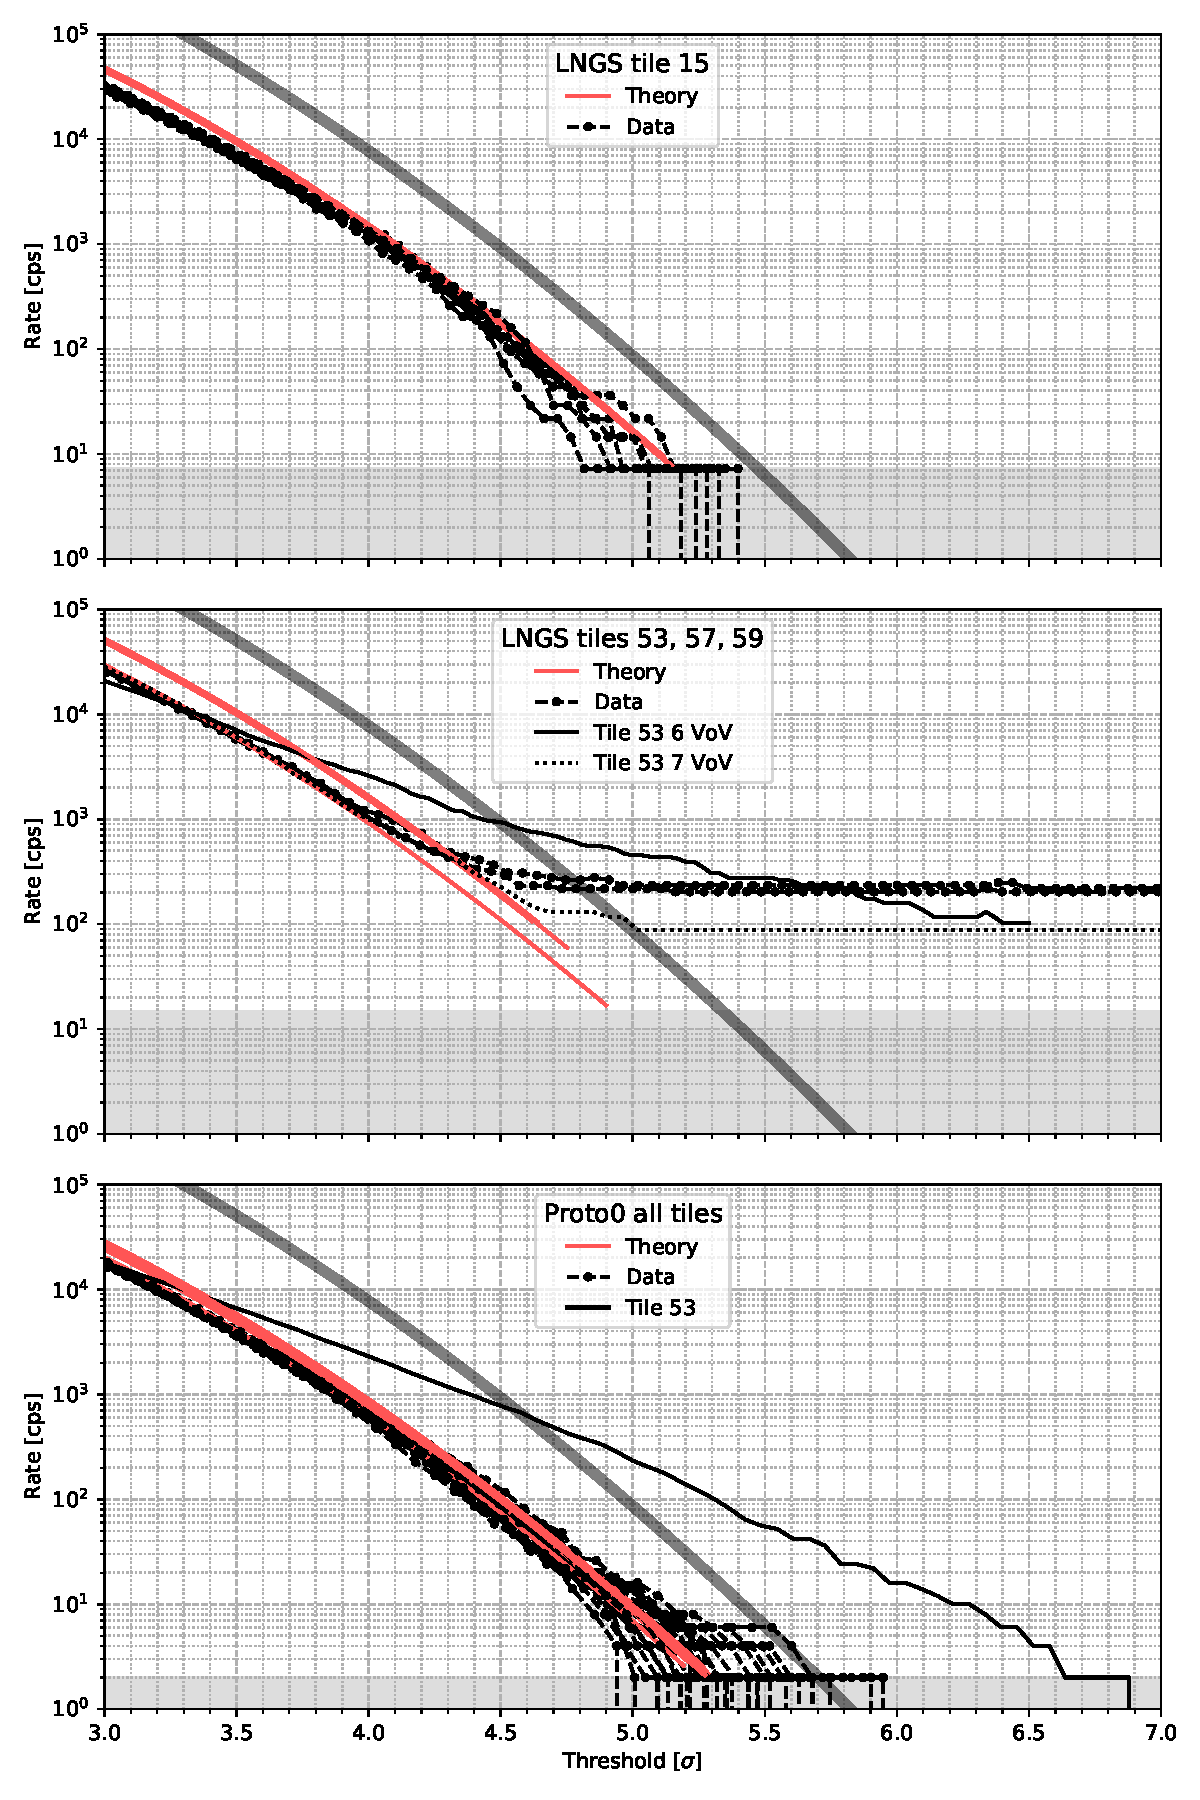
\includegraphics[width=1.25\textwidth]{figfakerate}
    
    \figcaption{fakerate}{The threshold upcrossing rate both counting directly
    the crossings on data and computing it with formula~\eqref{eq:rcont}. The
    gray band marks the rate corresponding to a single crossing counted in the
    data.}
    
\end{figure}

We didn't investigate further the discrepancy for tile~53. Anyway, for all
other tiles we looked at it works well enough.

We now want to estimate the minimum amount of data required for the procedure.
From \autoref{tab:fakerate} we see that the relative error on $k_2$ times the
square root of the time, $C \equiv
\operatorname{Std}[\bar{k_2}]\sqrt{T}/|k_2|$, is approximately \SI8{ns^{1/2}}
in all cases. The error should be proportional to $T^{-1/2}$, so to have an
\SI1\% error we need $T_{\SI1\%} = (100 C)^2 = \SI{0.7}{ms}$.

For convenience we summarize all the steps to compute the fake rate:
%
\begin{enumerate}
    
    \item Acquire \SI1{ms} of noise data.
    
    \item Filter the data (including baseline subtraction) producing a
    filtered waveform $\mathbf y$.
    
    \item Compute the standard deviation $\sigma$ and $k_2 =
    \operatorname{Cov}[y_i, y_{i+1} + y_{i-1} - 2y_i]$.
    
    \item Compute the fake rate for threshold $u$ using $r =
    f_s\sqrt{-k_2/(2\pi)}\operatorname{gauss}(u;0,\sigma)$ where $f_s$ is the
    sampling frequency.
    
\end{enumerate}
%
The probability of the formula not working due to mysterious reasons is \SI4\%.
If it works, the uncertainty for low rate is \SI{\pm50}\% and the result is an
overestimate with probability \SI{90}\%. (These assessments are based on
\autoref{tab:fakerate} but are somewhat subjective.)

Alternatively, if one has a noise spectrum available but not the noise
waveform, obtain the autocovariance by doing the discrete Fourier transform of
the power spectrum \cite[84]{ferrante2015} and then normalizing it to be
$\sigma^2$ in 0. Then $k_2$ is obtained by the covariance at lag 1 $c$ with
\eqref{eq:c2k2}. (If the spectrum was obtained from the discrete Fourier
transform of a noise waveform, $c$ is the first coefficient after the central
one in the autocovariance.)

    \chapter{Analysis of correlated SiPM noise}
\label{ch:anal}

In the previous chapters we studied the sources of noise in the procedure to
identify and measure a single signal. However the photodetector itself produces
pulses which are not due to a detected photon. There are two kinds of these:
pulses which are produced independently of incident light, and pulses which are
produced by another pulse. The latter case is called \emph{correlated noise}.

We will give a brief explanation and classification of the SiPM noise and then
analyze it on a specific tile with LNGS laser data. We will see that we can
reliably measure only the correlated noise, hence the chapter title.

There are two goals in characterizing the SiPM noise. First, a quantitative
model of the noise is needed for the DarkSide20k simulation, and we will
provide an estimate of the parameters for a recent new production of SiPMs.
Second, our ``direct'' analysis method that looks at each single pulse in a
complete recorded finely-sampled waveform provides a cross-check for more
indirect methods that will be employed online in the VETO system which has less
powerful readout electronics.

\marginpar{I should add some reference for charge integration methods. Maybe
the article where I found the Borel the first time, \cite{chmill2017}. I may
do this in the local conclusions.}

\section{Theory}

\marginpar{In chapter~\ref{ch:snr} I will add a qualitative description that
can be deduced from the 2d histogram without previous knowledge apart from the
acquisition setup (the laser position). Just as an epistemic exercise. I must
also add the definition of PE.}

In \autoref{ch:snr} we briefly introduced the Silicon Photomultiplier (SiPM).
We will now give a more detailed explanation, mainly following
\cite[ch.~3]{savarese2018}. For a general introduction to semiconductor
detectors (but not the SiPM), see \cite[ch.~11]{knoll2010}.

The difference between a SiPM and older kinds of semiconductor detectors is
that the SiPM has a binary response: the amplitude of the output is not
proportional to the energy released by the detected particle. In this sense
they are analogous to Photomultiplier Tubes (PMTs), because they are designed
to detect just the presence of a photon with high efficiency ($\sim\SI{50}\%$).

A SiPM is composed by a grid of \emph{cells}. The cells are Single Photon
Avalanche Photodiodes (SPADs). A SPAD is a photodiode operated in reverse bias
above its breakdown voltage in series with a \emph{quenching resistor}. Since
the bias is above breakdown, if a current starts in the photodiode it will be
self sustaining and would normally destroy the diode. The resistor in series
lowers the potential difference on the diode when a current flows through it,
stopping the current because the diode goes below breakdown, so the output
pulse will have duration and amplitude uniquely determined by the resistor and
the capacitance of the diode junction, independently of the initial release of
energy that triggered the current.

The difference between the bias and the breakdown voltage is called
\emph{overvoltage}, and is often indicated with the unit ``\si{VoV}'' meaning
``Volt overvoltage''.

The output from all the cells is summed analogically, so if multiple cells are
triggered simultaneously, the amplitude of the output pulse is discretized and
proportional to the number of fired cells. As we already said in
\autoref{ch:snr}, we will use the term ``PE'', standing for ``photoelectrons'',
as a unit when indicating the number of cells corresponding to a pulse.

\subsection{SiPM noise}

The initial creation of an electron-hole pair that starts the avalanche in the
photodiode can either be caused by an absorbed photon or by a thermal
fluctuation. The latter case happens randomly with fixed probability, and the
resulting rate of random pulses is called \emph{dark count rate}, where
``dark'' stands for the fact that this amounts to the total rate of pulses when
the photodiode is kept isolated from light.

The last sentence is actually not accurate because a ``primary'' pulse, either
a dark count or a photon, by various mechanisms can induce other pulses, that
can themselves recursively produce tertiary pulses in the same way. The four
ways in the proliferation of pulses are (see \autoref{fig:sipmnoise}):

\begin{description}

    \item[Afterpulses] During the avalanche, charge carriers can remain trapped
    into impurities and imperfections of the crystal. They are released
    afterwards at random, starting another avalanche in the same cell.
    
    \item[Direct cross talk (DiCT)] A photon emitted by an avalanche can
    trigger a nearby cell.
    
    \item[Delayed cross talk (DeCT)] Instead of hitting directly another cell,
    the photon can be absorbed in the shared crystal substrate and generate
    a hole that travels up until it passes through a cell and triggers it.
    
    \item[Delayed afterpulse] In the latter case, if the hole hits the
    originating cell, we call it delayed afterpulse instead of DeCT.

\end{description}

\begin{figure}
    
    \centering
    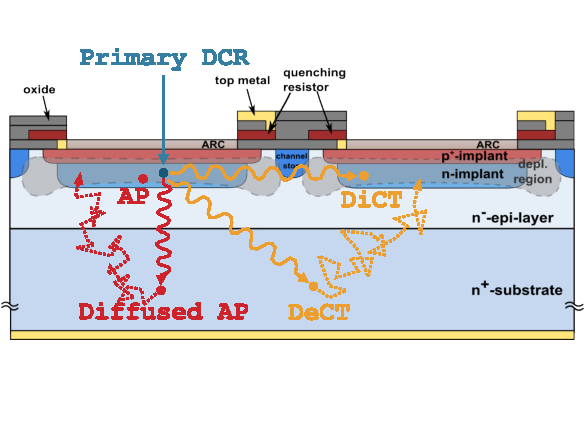
\includegraphics[width=0.85\textwidth]{sipmnoise}
    
    \caption{\label{fig:sipmnoise} Schematic of SiPM noises overlaid on the
    cross section of the device: AP (afterpulse), DiCT (direct cross talk),
    DeCT (delayed cross talk). From \cite[53]{savarese2018}.}
    
\end{figure}

The cells are less than \SI1{mm} wide, so the DiCT pulse starts within \SI1{ps}
of the originating pulse, while as we saw in \autoref{ch:snr} even just the
peak of the pulse lasts $\sim\SI{10}{ns}$. This means that the effect of the
DiCT is multiplying the height of the pulse by an integer factor, because the
overlapping pulses are well aligned. Afterpulses and DeCT, instead, can arrive
with a significative delay, and thus can be distinguished from the originating
pulse.

The reason why we classify separately the delayed pulses, instead of having an
overarching category of ``delayed noise'', is that afterpulses have a different
amplitude. The shape of the pulse is a sharp peak followed by an exponentially
decaying tail. This tail is due to the capacitance of the reverse-biased
junction that recharges through the quenching resistor after being discharged
inside the diode by the avalanche. A pulse generated by the same cell before
the recharge is complete can only use up the charge present in that moment.
Delayed cross talk, instead, has full amplitude because it involves a different
cell. See \autoref{fig:sipmnoiseampl}.

\begin{figure}
    
    \centering
    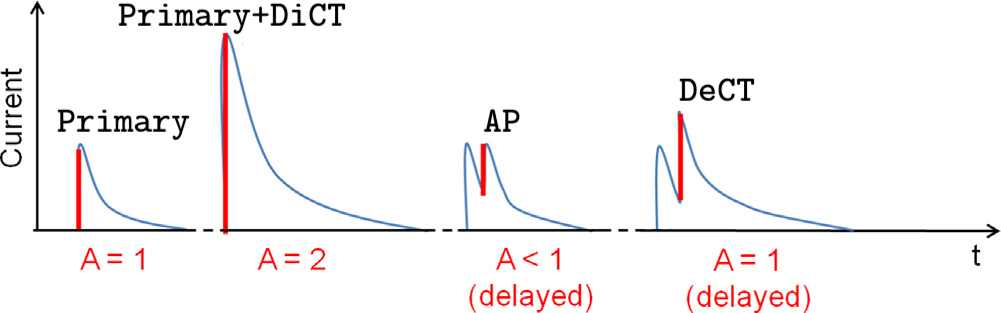
\includegraphics[width=0.85\textwidth]{sipmnoiseampl}
    
    \caption{\label{fig:sipmnoiseampl} Schematic of noise pulses. From
    \cite[4]{nagy2014}.}
    
\end{figure}

\subsection{DiCT model}

As we said, noise pulses can themselves produce other noise pulses as well. We
can imagine quite complicated interactions, for example: a DiCT induces a DeCT
on the original cell, thus producing a ``secondary'' delayed afterpulse. Or a
DiCT induces an afterpulse that induces a DiCT on the originating cell, again
with an afterpulse as final outcome. If the probabilities involved are small
enough, we should get by with the following simplifying assumption: that for
each pulse, the DiCT involves new cells that were not previously involved in
the chain, and the distribution of the number of DiCT at each step is fixed.

For the distribution to use for the generation model of DiCT, we follow
\cite{vinogradov2012}. Even when multiple DiCT steps are chained, the combined
delay is very small compared to the duration of the pulse, so the overall
effect of the complete DiCT ``tree'' is still to multiply the amplitude of the
first pulse. This means that at the end we just need to know the distribution
of the total number of consecutive DiCT.

For the single DiCT step, we consider two distributions: Bernoulli and Poisson.
In the first case we assume that a cell can induce a DiCT in at most just
another cell. In the second, we assume that there is a infinite population of
other cells, each with a fixed probability to be triggered. Clearly these two
cases are ``opposite'' approximations. In the first case, the distribution of
the total number of PE $k$ is Geometric. If $p$ is the probability of
generating a DiCT at each step, the distribution is
%
\begin{equation}
    P_G(k;p) = p^{k-1}(1-p), \quad k \ge 1, \quad p \in [0,1).
    \label{eq:geometric}
\end{equation}
%
Note that the conventional parametrization of the Geometric distribution is
different, with $p$ and $1 - p$ interchanged. We use this formulation because
it is more intuitively comparable with the other case. If the branching
distribution is Poisson with mean $\mu_B$, the total distribution is the Borel,
%
\begin{equation}
    P_B(k;\mu_B) = e^{-k\mu_B} \frac {(k\mu_B)^{k-1}} {k!},
    \quad k \ge 1, \quad \mu_B \in [0,1).
    \label{eq:borel}
\end{equation}
%
If it was $\mu_B \ge 1$, $k$ would diverge with nonzero probability.

The formula for the mean is formally the same for the two distributions,
%
\begin{equation}
    E[k] = \frac 1 {1 - p} = \frac 1 {1 - \mu_B},
\end{equation}
%
thus, since the interesting quantity is the amount of excess pulses due to
noise, it makes sense to compare the two distributions when $p = \mu_B$. We
make such comparison in \autoref{fig:geomborel} for $p = \mu_B = 0.5$. We note
that the Borel distribution has higher probability on the no-DiCT case, and at
the same time a fatter tail, while being lower in the few-DiCT cases.

\begin{figure}
    
    \widecenter{\includempl{figgeomborel}}

    \figcaption{geomborel}{Top panels: comparison of the geometric and Borel
    distributions (Equations~\ref{eq:geometric} and~\ref{eq:borel}), used for
    the total number of pulses in the DiCT tree, including the initial pulse.
    Bottom panels: geometric and generalized Poisson
    (Equations~\ref{eq:geompoisson} and~\ref{eq:genpoisson}), for the total
    number of PE when the number of initial pulses is Poisson distributed. The
    right panels are the same plots on the left in logarithmic scale.}
    
\end{figure}

Since we use laser data, there are multiple photons hitting the SiPM. The light
is diffused before reaching the photodetector (see \autoref{ch:data}), so we
expect at most one photon per cell, and thus a Poisson distribution for the
initial number of fired cells. So for the analysis we will need the
distribution of the total number of PE $n \ge 0$ for an initial
Poisson-distributed number of cells, each with its DiCT tree.

For the geometric model, the resulting distribution is called geometric Poisson
or Pólya-Aeppli. Let $\mu_P$ be the initial Poisson mean. The probability mass
function $P_{GP}$ can be computed with this recursion \cite[5]{nuel2008}:
%
\begin{align}
    P_n &\equiv P_{GP}(n;\mu_P,p), \\
    z &\equiv \mu_P \frac{1-p}p, \\
    P_0 &= e^{-\mu_P}, \\
    P_1 &= e^{-\mu_P} zp, \\
    P_n &= \frac{2n - 2 + z}n p P_{n-1} + \frac{2-n}n p^2 P_{n-2}.
    \label{eq:geompoisson}
\end{align}

For the Borel model, the distribution is the generalized Poisson:
%
\begin{equation}
    P_{BP}(n;\mu_P,\mu_B)
    = e^{-(\mu_P + n\mu_B)} \frac {\mu_P(\mu_P + n\mu_B)^{n-1}} {n!}.
    \label{eq:genpoisson}
\end{equation}

The means of the two distributions are, unsurprisingly, $\mu_P/(1-p)$ and
$\mu_P/(1-\mu_B)$. Note that for $n = 0$ the probabilities are equal, since
of course the cross talk does not affect the zero initial pulses case.

The referenced article finds a much better agreement with the Borel model when
looking at the tails of the PE distribution for DiCT only
\cite[p.~3~fig.~1]{vinogradov2012}, while it does not find a visible difference
for the Poisson+DiCT distribution with $\text{PE} \le 11$
\cite[p.~4~fig.~2]{vinogradov2012}.

\subsection{Afterpulse model}
\label{sec:aptheory}

For the afterpulses we have to model not just the number of pulses, but also
their temporal distribution and amplitude.

Afterpulses are produced by carriers trapped during the avalanche that get
released afterwards. Following \cite[1]{nagy2014}, we claim that this fact has
been proven by \cite{cova1991}, although by reading the latter article we feel
that their report is a bit too synthetic.

The release of trapped carriers is a thermodynamical process regulated by the
potential difference that the carriers must overcome to jump out of their
traps. This means that it also depends on the external bias. If there was only
one kind of trap, the temporal distribution of carrier releasing would be
exponential. However we expect to have various possible trapping energy levels,
so the distribution is in general a mixture of exponentials.

The released carriers also have a non-unitary probability of generating an
avalanche. This probability also depends on the electric field and thus on the
bias, like the release probability. The bias in turn depends on the recharge
state of the cell, thus deforming the exponential distribution for low delays.

While \cite[2]{nagy2014} tries to keep into account this deviation by
multiplying the afterpulse temporal distribution with the fraction of recovered
charge
%
\begin{equation}
    1 - \exp\left(-\frac{t}{\tau_\text{rec}}\right),
    \label{eq:recfactor}
\end{equation}
%
where $\tau_\text{rec}$ is the exponential scale of the pulse shape tail,
\cite[4]{garutti2014} goes straight with pure exponentials. However, we notice
from \cite[p.~5~fig.~11]{nagy2014}, reported here in \autoref{fig:nagyap}, that
they do not actually have data at low delays to test the accuracy of their
model, since the relatively high threshold they use for peak finding truncates
the afterpulse distribution at $\approx\SI{80}{ns}$. Even though the recharge
time is $\tau_\text{rec} = \SI{207}{ns}$, thus making the correction term
\eqref{eq:recfactor} significative even above the temporal cut, by looking at
the plotted histogram we think that a vanilla exponential with a different
amplitude and scale could fit as well.

\begin{figure}
    
    \centering
    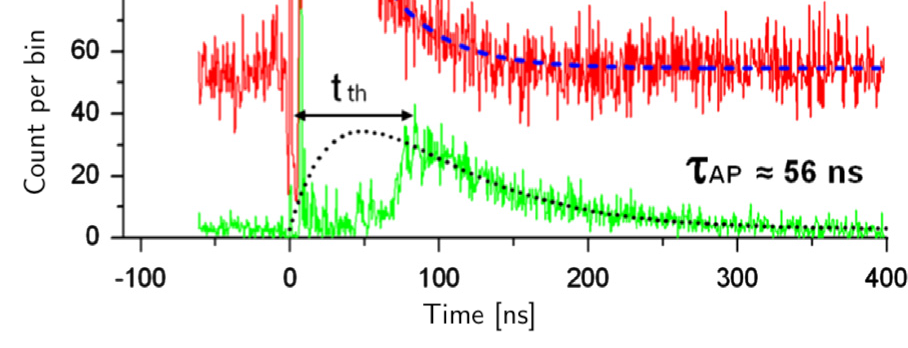
\includegraphics[width=\textwidth]{nagyap}
    
    \caption{\label{fig:nagyap} Excerpt of Figure~11 from \cite{nagy2014},
    showing the histogram of the delay of pulses successive to initial 1 PE
    pulses, selected with an upper bound on their amplitude to get afterpulses
    while removing dark count, and fitted with an exponential decay with
    constant $\tau_\text{AP}$ multiplied by the correction in
    \autoref{eq:recfactor} with $\tau_\text{rec} = \SI{207}{ns}$.}
    
\end{figure}

\cite{garutti2014} has approximately the same temporal cut and parameters, and
gets a good fit with either one or two uncorrected exponentials. We anticipate
that in our analysis the temporal cut will be even further relative to
$\tau_\text{rec}$ than in the referenced articles, so we will not be able to
discriminate the two models. For simplicity, we will keep the plain
exponentials.

The other matter with low delays is the amplitude reduction. Here all the
references we consulted agree on multiplying the 1 PE amplitude by the recharge
factor \eqref{eq:recfactor}, thus assuming that amplitude is proportional to
overvoltage. We will see this may not be accurate in our case.

Now to another topic: multiple afterpulses. The afterpulse avalanche itself
produces trapped carriers. However, since it may have smaller amplitude than a
primary avalanche, they will be less than those left around by a complete
discharge. Other two possible effects that we hypothesize, although we are not
sure about them, are: that if traps are not too far from saturation after an
avalanche, the additional afterpulses will be even more suppressed, and that an
avalanche may partially ``purge'' traps.

Keeping into account all these interactions is tedious, so we make a
simplifying assumption, inspired by the last consideration: that each avalanche
resets the cell to a fixed state. In this model, a pulse can have at most one
afterpulse. An eventual successive afterpulse must be produced by the first
afterpulse, not the initial pulse. \cite{cova1991} implicitly states that this
is not the case, although their experimental conditions are different because
the procedure they use to fill the traps is different from a ``spontaneous''
avalanche. Since these are second order effects, we anticipate that the
probabilities involved are small and that we probably would not be able to
falsify the simplified model with our data.

Bringing the DiCT model into the picture, each afterpulse will have its own
DiCT tree. We suppose that a smaller avalanche should emit less photons and
thus have less cross talk; again, for the sake of simplicity, we will assume
that the DiCT probability remains the same instead.

Since the DiCT involves separate cells, even with our ``resetting afterpulse''
model if the initial pulse has more than one PE then multiple afterpulses due
to the same initial pulse are allowed. We call this case \emph{parallel
afterpulses}, while the case with an afterpulse of an afterpulse \emph{series
afterpulses}.

\subsection{Expected values}
\label{sec:expval}

\cite[tab.~3.1~p.~62]{savarese2018} summarizes the noise parameters for the FBK
SiPMs at \SI{80}K and \SI{5}V overvoltage. In this analysis we will use newer
LFoundry SiPMs, so we can just get a rough idea from that. There are various
kinds of SiPM in the table, the low field near ultraviolet with medium
quenching resistance (last column) is the only one with the same recharge time
as ours ($\tau_\text{rec} = \SI{0.5}{\micro s}$) so we consider that values.
The dark count rate, converted from rate per area to rate per PDM (area
\SI{25}{cm^2}), is \SI{25}{cps}. The correlated noise probabilities are: DiCT
\SI{17}\%, AP \SI{17}\%, DeCT \SI{1.5}\%.

We did not make a model for DeCT (including delayed afterpulses) because we do
not have a clean selection of it in our data. In
\cite[fig.~3.8~p.~54]{savarese2018} we see that DeCT arrives within
\SI{50}{ns}. We will not properly analyze correlated pulses with delay below
\SI{100}{ns}. For the DeCT we will just give a very uncertain estimate. Since
the probability is smaller than the other noise modes, we completely neglect
second order effects due to DeCT.

\section{Data}

We use LNGS laser data for tile 21, produced by LFoundry. The LNGS data files
are:
%
\begin{verbatim}
LFOUNDRY/pre-production-test/TILE_21/LF_TILE21_77K_54V_65VoV_X.wav
LFOUNDRY/pre-production-test/TILE_21/LF_TILE21_77K_54V_69VoV_X.wav
LFOUNDRY/pre-production-test/TILE_21/LF_TILE21_77K_54V_73VoV_X.wav
\end{verbatim}
%
The `\texttt{X}' suffix in the file name stands for an index which goes from~1
to~10. Each file contains $\approx\num{20000}$ events, so we have \num{200000}
events per overvoltage.

The overvoltage is obtained by subtracting the first voltage from the second in
the file name and dividing by two. The first is the breakdown voltage while the
second is the applied reverse bias; the division is because the SiPM connection
layout in the PDM is parallel branches each with two SiPMs in series. Thus the
overvoltages are \SI{5.5}V, \SI{7.5}V, \SI{9.5}V.

We show the time-value histograms of a single file per overvoltage in
\autoref{fig:hist2dtile21}. These files do not include the laser trigger
waveform. Looking at the histograms it appears that the laser pulse arrives at
$\approx\SI{9}{\micro s}$ as usual. To be confident that we can assume the
trigger position, in \autoref{fig:triggerhist} we histogram all the triggers
from a lot of LNGS files. The full range of the distribution is
\SI[separate-uncertainty=true]{8969 \pm 11}{Sa}.

\begin{figure}
    
    \widecenter{\includempl{figtriggerhist}}
    
    \figcaption{triggerhist}{Cumulative histogram of the trigger leading edge
    (the first sample less than 600 in the recorded waveform) for 96 LNGS
    files. The distribution has the shape of a convolution between two uniforms
    with length 16 and~8, we suppose these are the clocks of the digitizer and
    laser triggers.}
    
\end{figure}

In some files there are double peaks in the fingerplot, i.e.~there are two
possible pulse amplitudes corresponding to the same number of PE. The worst
offender is the first file at \SI{5.5}{VoV},
\nolinkurl{LF_TILE21_77K_54V_65VoV_1.wav}. In \autoref{fig:doublepeak} we show
the fingerplot, both global and as a function of time, computed with
\SI{1.5}{\micro s} charge integration. It is evident that the pulse charge
changes during the acquisition. Since it is still possible to separate the PE
peaks, even if they are doubled, this will not be an issue. Moreover, with the
filter we will use in the analysis the doubling will be much less marked.

\begin{figure}
    
    \widecenter{\includempl{figdoublepeak}}
    
    \figcaption{doublepeak}{The distribution of the mean of the waveforms from
    sample 8958 to \num{10457} (1500 samples) in the first file at
    \SI{5.5}{VoV}. Left panel: global distribution. Right panel: the same
    distribution by groups of 200 events.}
    
\end{figure}

It was reported to us that in this data there could be a significative amount
of light that hits the detectors after being reflected. Since the apparatus is
small, we estimate an upper bound of \SI{1}m for the distance traveled by
light, which corresponds to a \SI{3}{ns} delay. This delay is smaller than
the scale of the variations of the signal shape and of the noise, so we can
neglect this problem.

\section{Peak finding}

As input to the analysis we will measure the amplitude and temporal position of
all the single pulses in the data. We will filter the waveforms to suppress
noise and then run a peak finding algorithm.

\subsection{Filtering}
\label{sec:filtering}

We filter each event using a cross correlation filter (see
\autoref{sec:filters}). We follow the procedure outlined in \autoref{ch:snr} to
make the filter template. We do the template separately for each file, to check
for unexpected variations in the pulse shape. The templates obtained are shown
in \autoref{fig:templates}. Although the variations appear to be reasonably
small, we use each template only for its own file.

\marginpar{Add more precise reference when I fix the template stuff.}

\begin{figure}
    
    \widecenter{\includempl{figtemplates}}
    
    \figcaption{templates}{Templates of the pulse shape obtained with averaging
    for each file.}
    
\end{figure}

An unexpected feature is the nonlinearity of the pulse amplitude with
overvoltage. A possible explanation is mislabeling of the overvoltages. The
overvoltage is determined from the bias and breakdown voltages reported in the
file name. The breakdown voltage is always the same because it is a property of
the tile, so if it was reported incorrectly, the correction to the overvoltage
would be a fixed offset. But in this case even if the ratio amplitude over
overvoltage would vary, the slope would be preserved, while in
\autoref{fig:templates} wee see that two equal overvoltage steps correspond to
clearly different absolute increases in amplitude.

One could think that the reported bias was incorrect, but it is a very simple
measurement. We will come back to this discussion after the analysis.

Filtering increases the signal to noise ratio, but degrades the separation
between close peaks. Since we are studying correlated pulses, it is thus
important to use a filter as short as possible. We filter the waveform with a
logarithmic range of filter lengths: \SI{32}{ns}, \SI{64}{ns}, \ldots,
\SI{2048}{ns}. The computations we will describe are carried in parallel with
all filter lengths, and then we choose in the analysis which lengths to use.
The truncation of the template to the desired length is done like in
\autoref{ch:timeres}, keeping the fixed length subrange of samples that has
maximum squared norm.

\marginpar{When I fix the template stuff, the chapter for the truncation will
be \autoref{ch:snr}.}

As usual the template is normalized to unit sum for filtering, such that the
filter behaves like an average and the baseline can be computed independently
of the filter. This also means that signals will stay negative.

To evaluate the filter near the boundaries, the waveform is prolonged with the
estimated baseline value, described in the next section. We defer to
\autoref{sec:pe} the description of how we select the filter length.

\subsection{Baseline}

To compute the height of the peaks we have to subtract the baseline value. We
compute the baseline using the pre-trigger region of the waveforms. For
robustness against deviations we use the median instead of the average. The ADC
has relatively low resolution (10~bit), so since the median can output only one
of the values of the input sequence it is quantized. To have a more continuous
output we divide the array in 8 interleaved subarrays, i.e.\ the first subarray
contains samples 0, 8, 16, \dots, the second 1, 9, 17, etc., take the median
separately on each subarray, and then average the medians.

If any pre-trigger sample in an event is less than 700, for that event we reuse
the baseline obtained in a previous event.

In \autoref{fig:baseline} we show the histogram of the obtained baseline values
for the \SI{5.5}{VoV} data. We will carry on the discussion always on the
\SI{5.5}{VoV} dataset as example, unless otherwise necessary.
Appendix~\ref{ch:analplot} contains additional plots that complete the picture.

\begin{figure}
    
    \widecenter{\includempl{figbaseline}}
    
    \figcaption{baseline}{Distribution of the waveform baseline measured in
    the pre-trigger region of the events. See \autoref{fig:baseline2} for all
    overvoltages.}
    
\end{figure}

The baseline distribution has a small tail to the left (note that the scale is
logarithmic) and some far outliers. In \autoref{fig:bsoutlier} and
\autoref{fig:bstail} we show the events corresponding to the lowest and highest
measured baselines and a pair of events from the lower tail respectively. (The
event visualization contains elements which we have not introduced yet, they
will soon be explained.)

\begin{figure}
    
    \widecenter{\includempl{figbsoutlier-0}\includempl{figbsoutlier-1}}

    \figcaption{bsoutlier}{The events with the lowest and highest baseline.
    See \autoref{fig:bsoutlier2} for all overvoltages.}

\end{figure}

\begin{figure}
    
    \widecenter{\includempl{figbstail-0}\includempl{figbstail-1}}

    \figcaption{bstail}{A pair of events from the low baseline tail (baseline
    between 955 and 956). See \autoref{fig:bstail2} for all overvoltages.}

\end{figure}

In all cases the extreme baseline events do not show anomalies, they have
genuinely unusual baselines. At \SI{5.5}{VoV} and \SI{9.5}{VoV} the events
corresponding to the lowest and highest baseline have close progressive
indices, so they must occur close in time; we suppose then that these
deviations are due to low-frequency transient oscillations.

The events in the tail all have a pre-trigger pulse (we checked only the two
ones we plotted, we did not handpick). This means that we will systematically
underestimate the amplitude of pre-trigger pulses. However, as is already
evident by looking at the event plots, the bias is small compared to the pulse
height. If data with lower SNR was to be processed, we would up the baseline
veto value from 700 to something as close as possible to the noise pedestal and
segment the baseline computation to detect inhomogeneity, but in our present
case we will go on without fixing this bias.

\subsection{Laser peak}
\label{sec:laser}

We know where the laser pulse should be, so we search it separately from other
pulses. We take a window from the filtered waveform of \SI{\pm 30} samples
around the expected trigger position 8969. In this window we take the minimum
local minimum, i.e.\ we consider the samples which have higher neighboring
samples, and take the minimum of these. If there is no local minimum, which
happens when the waveform is monotonically increasing or decreasing within the
60 selected samples, we mark the laser peak as missing.

To check that this is working we look at the distribution of the peak positions
for 1 PE pulses (\autoref{fig:laserpos}, left panel). It is centered on 8969 as
expected. However, it has a tail to the right when the filter length is short.
An explanation that comes to mind is that maybe when the SNR is not high
enough, the peak finder is picking up a close afterpulse instead of the main
peak. Given the short delay this should be unlikely, but since we are
particularly interested in afterpulses it is better to check this thoroughly.

\begin{figure}

    \widecenter{\includempl{figlaserpos-0}\includempl{figlaserpos-1}}

    \figcaption{laserpos}{Left panel: histogram of the laser peak position,
    only for 1 PE peaks, for all filter lengths. The zero of the scale is such
    that the expected position is 8969. Right panel: 2D histogram of the laser
    peak position and the amplitude, for the same selection of peaks, but only
    with the \SI{128}{ns} filter. See \autoref{fig:laserpos2} for all
    overvoltages.}
    
\end{figure}

As a first diagnostic, we look at the joint distribution of the peak position
and height (\autoref{fig:laserpos}, right panel). If the minimum was moving to
the right due to an additional close peak, we would expect a positive
correlation between height and position in the tail. Instead, we see a negative
correlation.

Then we look at the events themselves. In \autoref{fig:lptail} we show the
event with the rightmost position at \SI{64}{ns}, filtered with \SI{64}{ns} and
\SI{128}{ns}. With the longer filter the position goes back to the center of
the distribution. We inspected a lot of events in the tail and they are almost
all like the one we show.

\begin{figure}

    \widecenter{\includempl{figlptail-0}\includempl{figlptail-1}}

    \figcaption{lptail}{Left panel: the event with the rightmost laser peak
    position for 1 PE peaks with filter length \SI{64}{ns}. Right panel: the
    same event with filter length \SI{128}{ns}. See \autoref{fig:lptail2} for
    all overvoltages.}

\end{figure}

Finally, the tail contracts as the overvoltage increases (see
\autoref{fig:laserpos2}). From these observations we induce that the right
shift is caused by random fluctuation. The asymmetry of the tail reflects the
asymmetry of the shape of the signal.

We have not said how we are selecting 1 PE pulses. The explanation will come in
\autoref{sec:pe}. Also, we have talked about the positions of the peaks in the
filtered waveform without specifying the alignment of the filter output
relative to the input. For example, in the histogram (\autoref{fig:laserpos})
the position is centered on the assumed trigger 8969, while clearly in the
event visualization (\autoref{fig:lptail}) the peak search range is after the
trigger. The reader has to trust us that although we employ multiple
conventions, we use them consistently each time.

We said that with our procedure a laser peak can be missing. However we know
that the laser is always present; even when there are no pulses, we need to
count the event as a 0 PE laser signal to fit the Poisson+DiCT distributions.
We have to make something of the ``missing laser'' events.

First, we count these events for each filter length (\autoref{fig:missing},
left panel). They are about \SI{1.5}\% of the total, so not negligible. We went
through a lot of these events and they are almost all genuinely missing pulses.
It turns out that the noise is actually quite likely not to produce a local
minimum in a \SI{60}{ns} window after filtering. Nevertheless, there are some
events which have a pulse which for some weird combination of noise
oscillations is not detected properly.

\begin{figure}

    \widecenter{\includempl{figmissing}}
    
    \figcaption{missing}{Left panel: for each overvoltage, the fraction of
    events where there is no local minimum in the laser peak search range, as a
    function of filter length. Right panel: the fraction of events where the
    minimum is missing for all filter lengths less than or equal to the one on
    the abscissa.}

\end{figure}

As in the case of the right shift, the anomalies tend to appear only for a
particular filter length choice and disappear on the same event with other
lengths. So as a simple solution we use the shortest filter which yields a
non-missing peak when the preferred filter does not work. The right panel of
\autoref{fig:missing} shows how the fraction of missing events decreases as we
allow more lengths to choose from. Even with this fix, however, there is a hard
core of events which do not have a local minimum in any case; from \SI{0.03}\%
at \SI{5.5}{VoV} to \SI{0.15}\% at \SI{9.5}{VoV}.

These events are more interesting, so we show 12 of them at random for each
overvoltage in Figures~\ref{fig:verymissing0}, \ref{fig:verymissing1},
and~\ref{fig:verymissing2}. With our good old eyes, we identify three cases:
1)~true missing pulses, 2)~delayed pulses which fall out of the window, and
3)~pulses which are shadowed by a very high close consecutive pulse. In
\autoref{tab:missing} we list the total number of hard misses and the counts
of the three categories in the sample for all overvoltages.

\begin{table}
    
    \widecenter{
        \begin{tabular}{S[table-format=1.1] S[table-format=3] *3S[table-format=1]}
            \toprule
            & & \multicolumn3c{Count of 12} \\
            \cmidrule(l){3-5}
            {Overvoltage [\si{V}]} & {Total} & {True miss} & {Delayed} & {Close consecutive} \\
            \midrule
            5.5 &  56 & 4 & 3 & 5 \\
            7.5 & 148 & 7 & 5 & 0 \\
            9.5 & 303 & 5 & 0 & 7 \\
            \bottomrule
        \end{tabular}
    }
    
    \tabcaption{missing}{The number of events where the laser peak is missing
    with all filter lengths, and the counts, in a random sample of 12 of these
    events, for the three categories of configurations that appear in this
    selection.}
    
\end{table}

The delayed pulses could be photons that produce carriers in an inactive region
that then migrate to a diode junction (we are not sure about this, it is just
speculation). The consecutive pulses could be DeCT with high DiCT, they would
have the time scale we expect from \cite[fig.~3.8~p.~54]{savarese2018}
already mentioned in \autoref{sec:expval}, or less likely afterpulses.

Since these events are a small fraction of the sample we did not fix this
further. We will just keep in the back of our minds that there are these events
and check case by case that ignoring them has a negligible effect.

\subsection{Other peaks}

We identify other pulses using a prominence-based peak finder. With
``prominence'' we mean the topographical prominence, which is defined as
follows: starting from the peak whose prominence is to be measured, go to the
right and to the left until an higher elevation is found. For each side, take
the minima between these stops and the peak. The prominence is the difference
in elevation between the peak and the maximum of the two minima. See
\autoref{fig:prominence} for an illustration.

In this discussion we will use positive signal logic, so a peak is a local
maximum. Remember that in the actual analysis the convention is swapped.

\begin{figure}
    
    \widecenter{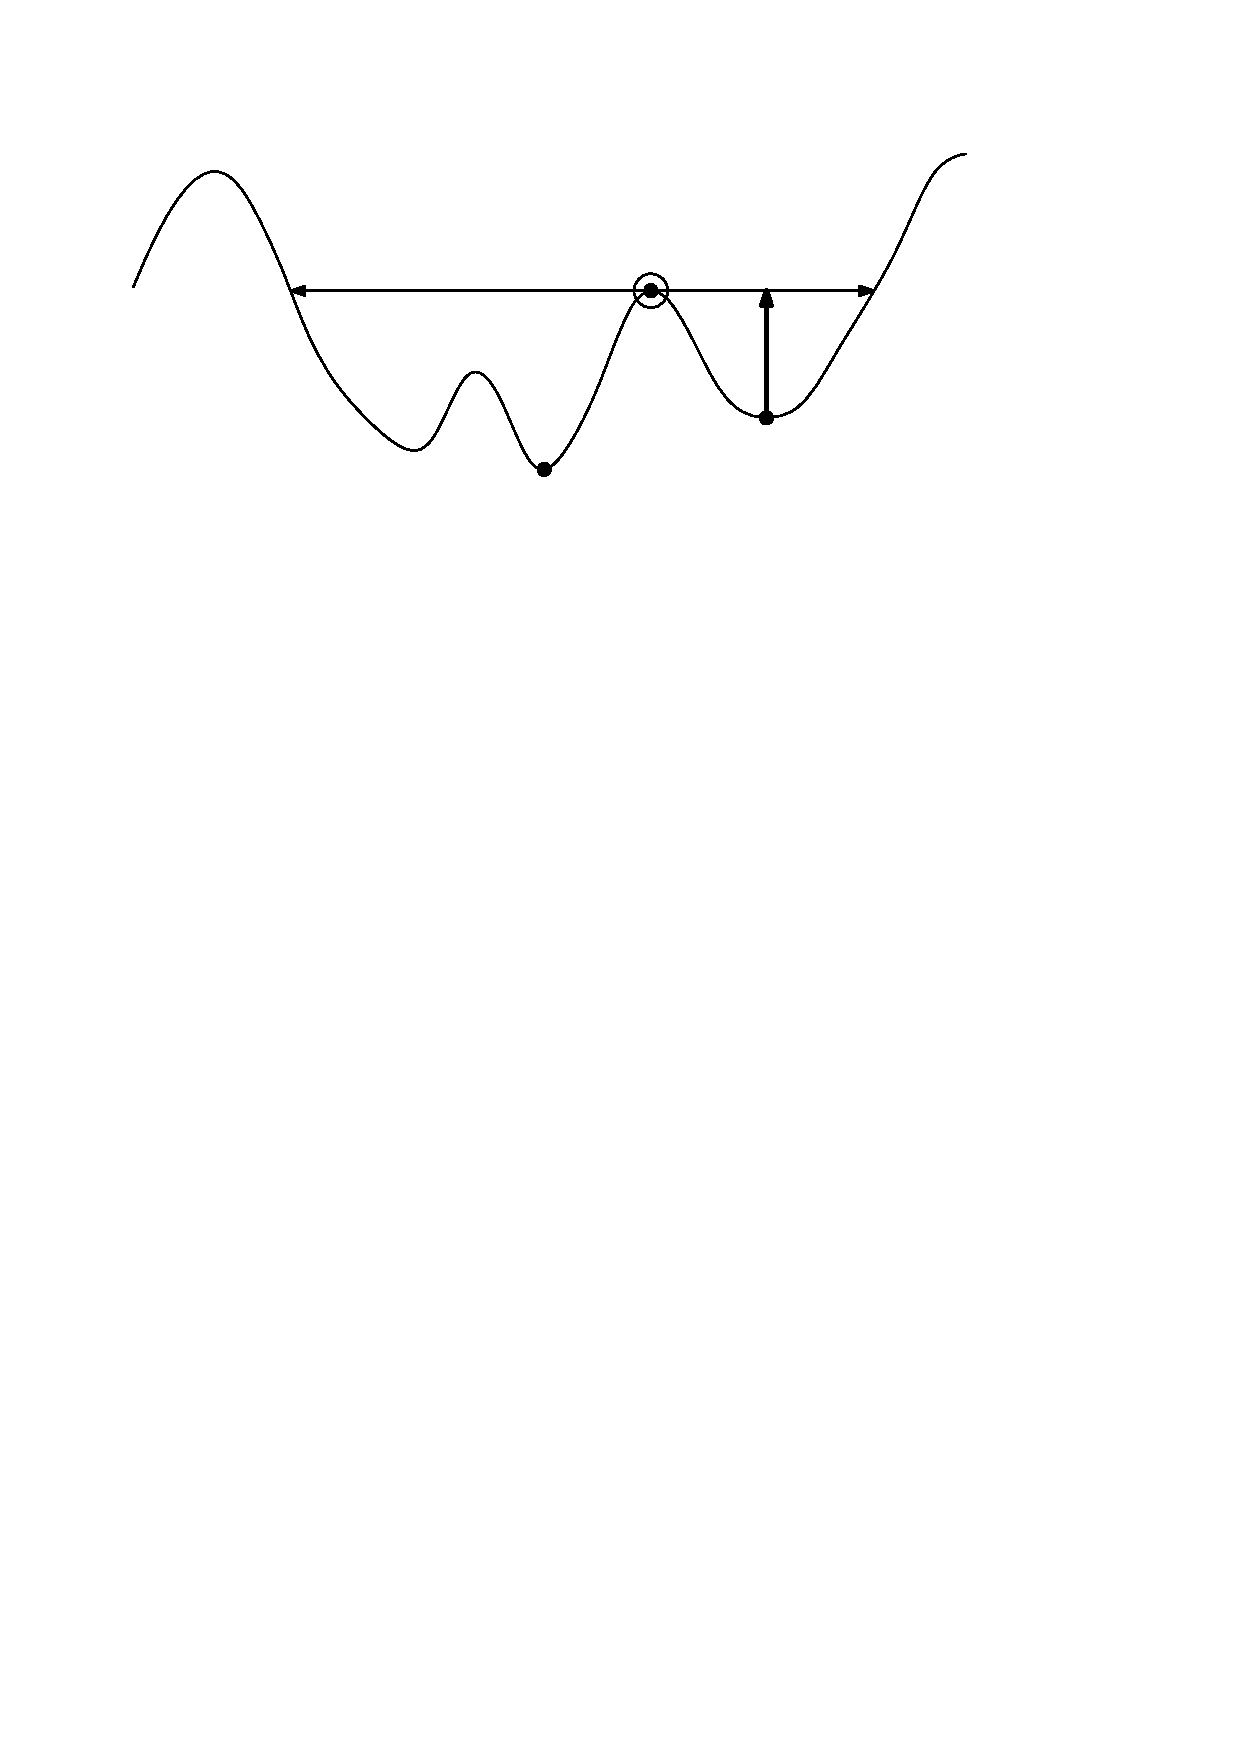
\includegraphics[width=0.8\textwidth]{prominence}}
    
    \caption{\label{fig:prominence} Illustration of the definition of
    topographical prominence. The prominence of the circled peak is the length
    of the thick vertical arrow.}
    
\end{figure}

We search the peaks separately in the pre and post laser peak regions. When the
laser peak is missing, we use the beginning of the laser peak search range as
separator. This means that even if the laser peak is lower than the peak, the
prominence ``exploration range'' stops there.

If one of the minima occurs at the edge, it is ignored and the prominence is
computed using the minimum on the other side, unless both minima occur at the
edge. This is to avoid assigning a very low prominence to a pulse whose shape
is truncated due to being close to a boundary.

The minima are capped to the baseline: if a minimum is lower than the baseline,
the value of the baseline is used instead to compute the prominence. This
increases the ratio between the prominence of close pulses to the one of
isolated pulses, because if the explored range is longer it is easier to find a
deeper random oscillation.

For each region, we save the two most prominent peaks. We do not make a
selection on the prominence, we always fill the four slots per event. In this
way we can observe the distribution of the height of random peaks and choose
a good threshold afterwards.

In peak finding algorithms it is customary to require a minimum distance
between peaks. This is to avoid picking up close high peaks due to random
oscillation that actually correspond to a single pulse. Selecting by prominence
avoids this problem if the waveform is smooth, because close peaks will have a
shallow dip between them and the prominence of the lower one will be measured
relative to that. Our waveforms are smooth on the scale of the filter length,
so it did not turn out necessary to add a distance criterion.

In \autoref{fig:peakfinder} we show two examples of events with close
afterpulses correctly identified.

\begin{figure}
    
    \widecenter{\includempl{figpeakfinder-0}\includempl{figpeakfinder-1}}
    
    \figcaption{peakfinder}{The events with the closest pair of pre-trigger
    pulses (left panel) and post-trigger pulse closest to the laser pulse
    (right panel) for at least 1 PE peaks.}
    
\end{figure}

\subsection{PE}
\label{sec:pe}

To assign the number of PE to the peaks we need to define bins for the height
of the peaks. We want to choose the filter length that yields the optimal
separation between PE in the height distribution. A longer filter suppresses
the random height fluctuation due to noise; at the same time, however, it picks
up afterpulses with the template tail, adding an upper tail to each PE height
distribution. Since the afterpulse probability increases with the number of PE
of the primary pulse, the distributions for 0 and 1~PE are the least touched.

In our analysis we will care particularly about selecting 1~PE pulses and
separating the afterpulses. So we use the following criterion: we take the
shortest filter that allows to clearly separate the 1~PE distribution. These
filter lengths are respectively \SI{128}{ns}, \SI{64}{ns}, \SI{64}{ns} for
\SI{5.5}{VoV}, \SI{7.5}{VoV}, \SI{9.5}{VoV}. We show the templates for these
lengths in \autoref{fig:trunc}.

\begin{figure}

    \widecenter{\includempl{figtrunc}}
    
    \figcaption{trunc}{The principal filter templates used in the analysis,
    shown unnormalized.}
    
\end{figure}

We tried selecting away the afterpulse tails using the peak finder to locate
afterpulses, however we did not manage to reduce them significantly. We
interpret this as the tail being composed mainly of close and short
afterpulses, that can not be recognized individually due to their low height.
Being located on the slope of the laser peak, the prominence of a close
afterpulse tends to be lower that that of an isolated pulse with the same
height. Thus the peak finder will always find two random peaks in the noise
with higher prominence than a short afterpulse, forbidding us to try to use an
aggressively low threshold with an high fake rate, since those afterpulses are
not even present in the peaks list.

There are other two minor factors that deform the height distribution: the
saturation of the digitizer, and pre-trigger pulses close to the laser one.
Thus we histogram the laser peak height excluding events with saturation and
events where the peak finder locates a pre-trigger pulse higher than~8 within
\SI{2.5}{\micro s} before the trigger using the longest filter. This
histogram is shown in \autoref{fig:pe} for \SI{5.5}{VoV} and \autoref{fig:pe2}
for all overvoltages.

\begin{figure}
    
    \widecenter{\includempl{figpe}}
    
    \figcaption{pe}{Histogram of the laser peak height, with a selection to
    avoid biased heights. The dotted lines are the boundaries of the PE bins.
    See \autoref{fig:pe2} for all overvoltages.}
    
\end{figure}

We place the PE bin boundaries taking the midpoints between the two most
distant consecutive heights in the range between each pair of consecutive
height distribution peaks. Heights above the last boundaries are not assigned a
number of PE, but they are not lost for the analysis, we will just use an
overflow bin when necessary. The ruler ticks that accompany the peaks in the
event visualizations are these boundaries.

Note the dips between the peaks in the histograms (the vertical scale is
logarithmic). The lowest bin count is at most~4 in all cases. Let us put a
rough upper bound on the contamination. There are more than \num{10000} events
per peak. Supposing a worst case with 25 bins with 4 counts each penetrating
into a neighboring peak, it gives \SI1\%. This means that it is surely less
than the Poisson error on the count for each PE. The 1~PE peaks are well
separated, with a row of 0 or 1~count bins around them, so we estimate a
contamination of \SI{0.01}\%.

\marginpar{I forgot to mention that doing this with the amplitude is the same,
and that anyway we are doing it with the amplitude.}

\subsection{Amplitude of close pulses}

When two pulses are close to each other, the height contains a contribution
from the tail of the other pulse. We need to compute the amplitude of the
single pulse, i.e.\ the height it would have if it was isolated. To simplify
the problem, we make the following assumptions:
%
\begin{enumerate}
    
    \item the position of a peak does not depend on the presence of other
    pulses;
    
    \item the shape of afterpulses is the same as normal pulses.
    
\end{enumerate}

About the first assumption: we have seen that the peaks in the output of the
cross correlation filter have a sharp cusp. A perfectly sharp cusp, even if
summed to a sloping shape, remains in the same position. A rounded peak,
instead, will move slightly in the uphill direction when summed to a slope.
Actually, given the short filters we are using, these cusps are not really
sharp. Look at the second panel of \autoref{fig:peakfinder}. The peak in the
square box has a radius of less than \SI{10}{ns}. By intuition we expect the
peak to drift less than its radius, so we estimate that the typical error will
be \SI{5}{ns}.

About the second assumption: it seems that in the literature this is implicitly
given for. But, as we said before, it depends on the assumption that the pulse
shape does not change with overvoltage, such that while the cell is recharging,
its behavior will just be the rescaled version of its fully charged self. In
\autoref{sec:filtering} we have seen that the pulse amplitude does not depend
linearly on overvoltage. If you look closely at \autoref{fig:templates}, you
can notice that the shapes are also a bit different. We make a clearer
comparison in \autoref{fig:shape} by plotting the templates normalized to have
the same peak amplitude. They are indeed different, but the difference is small
enough to justify the working hypothesis.

\begin{figure}
    
    \widecenter{\includempl{figshape}}

    \figcaption{shape}{The signal templates at different overvoltages compared
    fixing the peak amplitude to~1. The thickness of the stroke is twice the
    standard deviation over the 10 files per overvoltage, while the center of
    the stroke is the mean.}
    
\end{figure}

Now, let $\mathbf y$ be the output of the filter applied to a single noiseless
pulse, which we compute by filtering the signal template. Let $t_\alpha$ be the
position of peak $\alpha$ and $a_\alpha$ the unknown amplitude. Since the
filter is linear, the filtered sum of the pulses and the noise is the sum of
each component filtered separately, so the model for the complete filtered
waveform $\mathbf w$ is
%
\begin{equation}
    w_i = \sum_\alpha a_\alpha y_{i - t_\alpha} + \epsilon_i,
\end{equation}
%
where $\boldsymbol\epsilon$ is the filtered noise. There is some freedom in the
definition of $\mathbf y$: we fix that the peak occurs at $y_0$ and that $y_0 =
1$, such that if there is only one peak then $w_{t_1} = a_1 + \epsilon_{t_1}$.

It is well known that the minimum variance in estimating $\mathbf a$ is
obtained by using least squares with the inverse of the covariance matrix $V$
of $\boldsymbol\epsilon$ as quadratic form. Let $H_{i\alpha} = y_{i-t_\alpha}$,
then the solution is \cite[628]{zyla2020}
%
\begin{equation}
    \hat{\mathbf a} = (H^\top V^{-1} H)^{-1} H^T V^{-1} \mathbf w.
    \label{eq:lsq}
\end{equation}
%
We note, however, that to solve the system it is just necessary to have as many
datapoints as the number of peaks. It then comes natural to solve for
simplicity this system of equations instead:
%
\begin{equation}
    w_{t_\beta} = \sum_\alpha \hat a_\alpha y_{t_\beta - t_\alpha},
    \label{eq:amplsystem}
\end{equation}
%
i.e.\ we use only the observed peak heights $w_{t_\beta}$ instead of the full
waveform.

What are we losing with this simplification? In \autoref{sec:filters} we said
that the matched filter is equivalent to linear least squares. We now indeed
show that, if we were using the matched filter, solving \eqref{eq:amplsystem}
would be equivalent to least squares and thus optimal. Just for this proof, let
us use all the above notation, but without the filter applied, i.e.\ $\mathbf
w$ is the unfiltered waveform, $\mathbf y$ is the unfiltered signal, $V$ is the
covariance of the unfiltered noise.

The template of the matched filter is
%
\begin{equation}
    \mathbf h = V^{-1} \mathbf y.
\end{equation}
%
The model (noise implicit) is
%
\begin{equation}
    \mathbf w = H \mathbf a.
\end{equation}
%
The filter is applied by operating with the matrix
\begin{equation}
    F_{ij} \equiv h_{j-i} = V^{-1}_{j-i,k} y_k,
\end{equation}
%
so applying the filter we have
%
\begin{align}
    F \mathbf w &= F H \mathbf a. \label{eq:noindices}
\end{align}
%
We want to use only the peak heights in the filter output, assuming that we
know exactly the true signal positions. These are
%
\begin{equation}
    W_\beta \equiv (F \mathbf w)_{t_\beta} = V^{-1}_{j-t_\beta,k} y_k w_j. 
\end{equation}
%
The noise is stationary, so we can sum the same offset to the indices of
$V^{-1}$. Using this fact, the symmetry of $V$, and redefining the mute index
$k$, we obtain

\marginpar{This translation of the indices of $V^{-1}$ holds only in the limit
of an infinitely long waveform. In practice for a waveform with some margin
around the pulses. However the initial mistake was not translating properly the
indices of $V^{-1}$ when defining the filter template; after fixing that it
should not be necessary to translate them later.}

\begin{equation}
    W_\beta = V^{-1}_{jk} y_{k-t_\beta} w_j = V^{-1}_{jk} H_{k\beta} w_j
    \rightarrow \mathbf W = H^\top V^{-1} \mathbf w.
\end{equation}
%
So, considering only the $W_\beta$ on the left hand side of
\eqref{eq:noindices} and putting the indices on the right hand side, we have
%
\begin{align}
    W_\beta &= V^{-1}_{j-t_\beta,k} y_k H_{j\alpha} a_\alpha = \\
    &= V^{-1}_{j,k} y_{k-t_\beta} H_{j\alpha} a_\alpha = \\
    &= (H^\top V^{-1} H)_{\beta\alpha} a_\alpha,
\end{align}
%
thus the solution is
%
\begin{equation}
    \mathbf a = (H^\top V^{-1} H)^{-1} H^\top V^{-1} \mathbf w,
\end{equation}
%
which is the least squares estimator \eqref{eq:lsq}. \hfill $\square$

Our filter differs in two ways from the matched filter: it does not keep into
account the noise correlation, and it is truncated. So our method for computing
the amplitude is worse than the optimal one as much as the filter is worse than
the matched filter.

In each event we have to decide which peaks to input in \eqref{eq:amplsystem}.
Most of the time, peaks are random noise oscillation. If the amplitude of
random peaks had mean zero, adding a fake peak would increase the error but not
introduce a bias. But, since we are selecting peaks by highest prominence, it
is guaranteed that in a region of some microseconds we will find a peak with
height comparable to the noise standard deviation. Indeed in the next section
we will look at the height distribution for the peak finder output and see that
it is positively biased. So we compute the amplitude only for peaks higher than
a threshold. As threshold we pick the the PE bin boundary between 0 and 1~PE.

When we use the computed pulse amplitude instead of the peak height, we would
like to also see the distribution of the fake peaks such that we can be sure at
a glance that we have no contamination, but most of the fake peaks do not have
an amplitude since they do not pass the threshold prerequisite. The $y$
normalization we have chosen makes the amplitude ``have the same units'' of the
height, so we construct a variable which is the amplitude when available, and
the height otherwise. In the following sections we mean this variable when we
talk about ``amplitude''.

Note that with this selection we are not excluding short afterpulses from the
amplitude computation, because even if their amplitude is smaller, sitting on
the tail of their parent pulse their height is still above threshold.

In the event visualizations, the ruler associated to each peak starts from a
dot placed such that the distance from the dot to the peak is the amplitude.
In the legend, the amplitude is given under ``$a = \ldots$''.

\section{Random pulses rate}

When counting afterpulses there will be a background from the dark count rate,
which we have to subtract, so we measure it in the pre-trigger region. The
laser trigger frequency should be less than \SI{1}{kHz}, so the events are
distant between each other and there is not the possibility of correlated noise
from a laser pulse leaking into the successive event.

\marginpar{What is the laser trigger rate? Specify this better if I know after
writing \autoref{ch:data}.}

The title of this section reads ``random pulses rate'' instead of dark count
rate because we will see we have reason to believe that in the data there are
actually more random pulses than the dark count. It does not matter for
background subtraction though.

By looking at the time-value histograms in \autoref{fig:hist2dtile21} we see
that in \num{20000} events there are just a few pre-trigger pulses, so we
neglect the case of a double random pulse in the same event. If there are two
pre-trigger pulses, one must be the afterpulse of the other, so the event
counts as one random pulse. For the rate we do not care to know which pulse is
the primary, but we will need it when fitting the DiCT model to the random
pulses.

The primary pulse is of course the first in chronological order, but to
distinguish the one pulse from the two pulses case we are forced to put a
threshold on the amplitude before looking at the distribution. We do something
similar as we did for the amplitude. The initial variables are the position,
height and amplitude of the two most prominent pre-trigger peaks. When both
heights are above the 0 to 1~PE boundary, the first set of variables is set to
the first peak in chronological order; otherwise to the most prominent peak.

In the left panel of \autoref{fig:pretrigger} we show the scatter plot of the
first pulse amplitude versus position. There are some problems at the edges. On
the left edge, the negative amplitudes are actually very large values that we
mapped to \num{-10}. They are probably due to the amplitude linear system
\eqref{eq:amplsystem} being degenerate, but we did not investigate why this may
happen. On the right edge conversely there are some zeroes and anomalously
small values. Thus we ignore the first \SI{100}{ns} and the last \SI{500}{ns}
of the pre-trigger region. The wider margin on the right is just to be safe in
case the presence of the laser pulse was having some effects. The selected
region is marked by the gray vertical band in the plot.

\begin{figure}
    
    \widecenter{\includempl{figpretrigger-0}\includempl{figpretrigger-1}}
    
    \figcaption{pretrigger}{Left panel: scatter plot amplitude vs.\ position of
    the chronological first pre-trigger peak in each event. Right panel:
    histogram of the amplitude for the peaks contained in the vertical gray
    band in the left plot. See \autoref{fig:pretrigger2} for all overvoltages.}
    
\end{figure}

The right panel of \autoref{fig:pretrigger} shows the histogram of the
amplitude of the pulses in the temporal cut. The separation between random
peaks and 1~PE pulses is clear; the amplitude threshold we use is marked with a
gray band also reported in the left panel. The dotted lines are the PE bin
boundaries. As we anticipated, the distribution of the amplitude of the random
peaks is biased upward, and leaks a bit above the 0 to 1~PE boundary.

To compute the rate, we count the number of pulses satisfying the cuts, and
divide by the number of events times the pre-trigger region duration minus the
cuts. The uncertainty is given by the Poisson error of the count. In
\autoref{tab:ptrate} we report the obtained values.

\begin{table}
    
    \widecenter{
        \raisebox{-0.5\height}{\includempl{figptrate}}
        \begin{tabular}{
            S[table-format=1.1]
            S[table-format=6]
            S[table-format=1.2]
            S[table-format=1.2]
            S[table-format=3]
            S[table-format=3(2), separate-uncertainty=true]
        }
            \toprule
            &
            & \multicolumn2c{Time}
            & \multicolumn2c{Pulses} \\
            \cmidrule(lr){3-4} \cmidrule(l){5-6}
            {Overvoltage}
            & {Events}
            & {Per event}
            & {Total}
            & {Count}
            & {Rate} \\
            {[\si V]}
            &
            & {[\si{\micro s}]}
            & {[\si s]}
            &
            & {[\si{cps}]} \\
            \midrule
            5.5 & 200028 & 8.37 & 1.67 &  73 &   44 \pm 5 \\
            7.5 & 200021 & 8.37 & 1.67 & 277 & 165 \pm 10 \\
            9.5 & 200025 & 8.37 & 1.67 & 186 &  111 \pm 8 \\
            \bottomrule
        \end{tabular}
    }
    
    \tabcaption{ptrate}{The rate of primary pre-trigger pulses in a fiducial
    region and the intermediate quantities used to compute it.}
    
\end{table}

We notice that the rate at \SI{7.5}{VoV} is substantially higher than the one
at \SI{9.5}{VoV}. The dark count rate steadily increases with overvoltage (see
for example \cite[fig.~3.13~p.~61]{savarese2018}), because an higher field in
the diode lowers the potential barrier that a carrier must overcome to become
conducive. So we induce that there must be an additional source of random
pulses. Maybe the experimental setup was not light-tight. Anyway, these values
can be considered an upper bound for the dark count rate. For reference, the
maximum dark count rate allowed by the DarkSide20k specifications is
\SI{250}{cps} \cite[tab.~3.1~p.~62]{savarese2018}.

\section{Afterpulses}

To study afterpulses we consider the post-trigger peaks in events with a 1~PE
laser pulse. Using the terminology introduced at the end of
\autoref{sec:aptheory}, a single PE initial pulse implies that there are no
parallel afterpulses. The parameter we are interested in is the probability for
a single cell to generate an afterpulse, thus even if there are two series
afterpulses, we only care about the first. So, like we did for pre-trigger
peaks, when there are two peaks with height above the 0 to 1~PE boundary we
select the first.

The case with an afterpulse and a random pulse is quite unlikely. From
\autoref{tab:ptrate} we compute that the probability of having a random pulse
in the post-trigger region is within \SI{0.1}\%. We will see that the
probability of an afterpulse is about \SI{5}\%, so the coincidence probability
is less than \SI{0.005}\%, in less than \num{50000} events, so we expect less
than 2.5 afterpulse+random events. Since the distribution of randoms is flat,
while the afterpulses are concentrated at short delays, and keeping into
account that even if both were uniform in half of the cases the afterpulse
would come first by chance, we are sure that the expected afterpulses lost due
to random are less than 1 and so we neglect this problem.

The amplitude of the afterpulses is shorter than normal at low delays. It would
be convenient to select them with a straight cut. This will be even more useful
when fitting the DiCT model on the afterpulses. We empirically observe that the
height of the afterpulses is approximately constant, although a bit higher at
short delays, like if the rule was that an afterpulse reaches a normal height
when ``sitting'' on the tail of its parent (see the top right panel of
\autoref{fig:apampl}). The slight increase for close pulses can be interpreted
as an effect of the smearing of the filter. So we do the following: we take the
\emph{unfiltered} signal template, normalize it to have peak amplitude as a
1~PE \emph{filtered} pulse, take its value at a delay from its peak equal to
the delay from the post-trigger to the laser peak, and sum this to the
post-trigger pulse amplitude.

\begin{figure}
    
    \widecenter{\includempl{figapampl-0}\includempl{figapampl-1}}

    \widecenter{\includempl{figapampl-2}\includempl{figapampl-3}}
    
    \figcaption{apampl}{Various ways of measuring the magnitude of post-trigger
    pulses. Top left: the prominence computed by the peak finder; it decreases
    with short delays so it does not allow a straight cut. Top right: the
    height from the baseline; it is straighter but leaks a bit above the 2~PE
    threshold. Bottom left: the amplitude; it yields a better separation than
    the prominence but has to be rectified. Bottom right: the corrected
    amplitude which we use in our analysis.}
    
\end{figure}

The obtained \emph{corrected amplitude} is shown in the bottom right panel of
\autoref{fig:apampl}. Note that this correction is not equivalent to dividing
by the expected recharge factor \eqref{eq:recfactor}, it is just an empirical
procedure that rectifies the observed distribution. This may indicate that the
model is inaccurate, however we did not investigate further. In the event
visualizations, the amplitude shown for post-trigger pulses is actually the
corrected amplitude.

We can now discuss an additional issue with selecting the first peak when there
are two of them. Before computing the amplitude we select by height. Pulses
sitting on the tail of the laser pulse have a height bonus, and we said this is
useful to avoid selecting away short afterpulses at this stage. However some of
these short pulses will turn out to be noise. If it happens that there is a
second true pulse, it will be hidden by the first noise pulse. So we take the
first chronological only when both have their corrected amplitude above the 0
to 1~PE threshold. We checked that at \SI{5.5}{VoV} there would be at most 13
cases with this problem, to be compared to about 500 selected post-trigger
pulses, so the effect would be small anyway.

To select the afterpulses we have to ignore short delays because we can not
separate too short pulses from the noise, and because the peak finder could be
losing some pulses if they are short and close to the laser peak. Moreover,
like with the random pulses, the threshold on the corrected amplitude has to be
set higher that the 1~PE boundary because the amount of noise is overwhelming
compared to the pulses. We also truncate the delay distribution at
approximately \SI{500}{ns} from the end of the waveform just to stay safe from
boundary effects. We first do the temporal selection, and then determine the
threshold with our usual procedure of taking the midpoint between the two most
distant consecutive samples. These selections are shown in
\autoref{fig:apscatter}.

\begin{figure}
    
    \widecenter{\includempl{figapscatter-0}\includempl{figapscatter-1}}

    \figcaption{apscatter}{Left panel: corrected amplitude versus delay from
    laser peak; the gray bands mark the selected ranges. Right panel: the
    histogram of the amplitude for the points that fall in the vertical band in
    the scatterplot. See \autoref{fig:apscatter2} for all overvoltages
    and a zoom in of the scatterplot.}
    
\end{figure}

We have done a temporal cut, thus to count the afterpulses we have to calculate
how many we have lost. To do this we need to determine the temporal
distribution and compute the probability mass that falls outside of the
selected range. We histogram the delay of the pulses and fit two distributions,
one with an exponential decay component and one with two.

Since we are selecting the first pulse after the laser peak, normally it would
be necessary to correct the distribution for a ``first arrived'' effect: an
eventual second pulse would not be counted, so the observed counts decay faster
with delay than the actual distribution. Simple example: start from a uniform
distribution, and take the first event after a fixed point in time; the
distribution transforms into the well known exponential. \cite[2]{cova1991} and
\cite[4]{garutti2014} both take this into account. In our case, however, we
have a model where caring only about the first pulse is ``built-in'' so to say.
Just for reference, asymptotically the correction would amount to the
probability of afterpulses, which as we will see is about \SI{5}\%.

This is not true for the background of random pulses, which would need the
correction, but its probability is so small that the correction can be
neglected. In other words: we approximate the exponential background of random
pulses with a uniform because the rate is very low compared to the observed
time interval.

We do an approximate Bayesian fit using least squares. This is described in
detail in \autoref{ch:fit}; for the impatient, just consider that this is
almost a standard least squares fit of a histogram, with additional squared
terms that represent the prior.

The priors of the fit are:
%
\begin{itemize}
    
    \item The expected uniform background, computed from the random pulse rate
    in \autoref{tab:ptrate}. The variance is determined only from the variance
    of the rate; the afterpulse count i.e.\ the histogram normalization is an
    errorless input.
    
    \item For the one component fit, the prior on the logarithm of the
    exponential decay constant in nanoseconds is $\log(1000) \pm 1$. Consider
    than a $\pm 1$ error on the natural logarithm corresponds to a \SI{100}\%
    relative error with first order propagation.
    
    \item For the two components fit, the priors on the logarithms are
    $\log(400) \pm 1$, $\log(800) \pm 1$, while the prior on the relative
    weight of the short component is a uniform in $(0, 1)$.
    
\end{itemize}

All the parameters are bounded, so they are fit transformed. The background
density and the exponential scales are transformed with the logarithm, while
the component weight is mapped to the unitary interval using the error
function, which makes the prior on it uniform.

Since the density varies a lot over the observed range of about \SI{5}{\micro
s}, we use uneven bins for the fit. As simple criterion we compute the bins
that would yield uniform counts with an exponential with scale \SI{1.5}{\micro
s}:
%
\begin{equation}
    b_i = t_L - \tau_0 \log\left(1 - \frac in
    \left(1 - \exp\left(-\frac{t_R - t_L}{\tau_0}\right)\right)\right),
    \quad i = 0, \ldots, n,
\end{equation}
%
where there are $n$ bins, $b_i$ is the $i$-th bin edge, $\tau_0 =
\SI{1.5}{\micro s}$, and $(t_L, t_R)$ is the total range. For $n$ we take 3/4
of the square root of the total count. With these criteria it never happened
to have a bin with a count less than~5.

We are using somewhat large bins, so we have to fit against the integral of the
distribution instead of the usual approximation of taking the density in the
center of the bin. The cumulative density functions for the two models are:
%
\begin{align}
    P_1(t_L < t' < t;\tau,R) &=
    \left(1-\frac RN\right)
    \left(1 - e^{-t/\tau}\right)
    + \frac RN \frac t{t_R-t_L}, \\
    %
    P_2(t_L < t' < t;\tau_1,\tau_2,p_1,R) &=
    \left(1-\frac RN\right)
    \left[p_1 \left(1 - e^{-t/\tau_1}\right)\right. \notag \\
    \phantom x &+ \left.(1 - p_1)
    \left(1 - e^{-t/\tau_2}\right) \right] \notag \\
    \phantom x &+ \frac RN \frac t{t_R-t_L},
\end{align}
%
where $\tau$, $\tau_1$ and $\tau_2$ are the exponential scales, $p_1$ is
the weight of the component with the shorter prior, $R$ is the number of
random pulses, and $N$ is the total histogram count.

Once we have the fitted parameters, we correct the afterpulse count by
subtracting the fitted background and dividing by the probability mass
contained in the range:
%
\begin{align}
    N_1 &= \frac {N-R} {\exp(-t_L/\tau) - \exp(-t_R/\tau)},
    \label{eq:n1} \\
    %
    N_2 &= \frac {N-R} {p_1 (e^{-t_L/\tau_1} - e^{-t_R/\tau_1})
    + (1-p_1) (e^{-t_L/\tau_2} - e^{-t_R/\tau_2})},
    \label{eq:n2}
\end{align}
%
then we divide by the number of events to compute the afterpulse probability.
In \autoref{fig:apfit} we show the fit, while in \autoref{tab:ap} and
\autoref{fig:apresults} we summarize the results for all overvoltages. In all
the calculations, when necessary, we have kept into account the correlations to
propagate the error.

\marginpar{It may be useful to compute the number of afterpulses weighted with
the amplitude, since the afterpulses get denser as they get shorter.}

\begin{figure}
    
    \widecenter{\includempl{figapfit-0}\includempl{figapfit-1}}

    \figcaption{apfit}{Left panel: fit of the temporal distribution of
    post-trigger pulses. Right panel: the histogram with even bins and without
    the temporal cuts. In the legend, `const' is the background excess density,
    i.e.\ $(R/N)/((t_R-t_L)(1-R/N))$, in \si{ns^{-1}}. See \autoref{fig:apfit2}
    for all overvoltages.}
    
\end{figure}

\begin{table}
    
    \widecenter{
        \scriptsize\sffamily
        \setlength\tabcolsep{4pt}
        \begin{tabular}{
            S[table-format=1.1]
            S[table-format=3]
            S[table-format=4]
            S[table-format=5]
            S[table-format=3]
            S[table-format=1.2]
            S[table-format=2.1(2)]
            S[table-format=2.1(2)]
            S[table-format=3(2)]
            S[table-format=1.2(2)]
            S[table-format=2.1(2)]
            S[table-format=1.3(2)]
            S[table-format=1.2(2)]
            S[table-format=3]
            S[table-format=2]
            S[table-format=1.2]
        }
            \toprule

            & \multicolumn2c{Delay range}
            & {}
            & {}
            & {}
            & {}
            & \multicolumn4c{Fit parameters}
            & {}
            & {}
            & \multicolumn3c{Fit quality} \\
            \cmidrule(lr){2-3} \cmidrule(lr){8-11} \cmidrule(l){14-16}
            {OV}
            & {tL}
            & {tR}
            & {Events}
            & {N}
            & {Time}
            & {R prior}
            & {R}
            & {tau1}
            & {tau2}
            & {p1}
            & {Correction}
            & {Prob.}
            & {chi2}
            & {dof}
            & {pvalue} \\
            {[\si V]}
            & {[\si{ns}]}
            & {[\si{ns}]}
            &
            &
            & {[\si s]}
            &
            &
            & {[\si{ns}]}
            & {[\si{\micro s}]}
            & {[\si\%]}
            &
            & {[\si\%]}
            &
            &
            & \\
            \midrule
5.5 & 250 & 5500 & 46990 &  620 & 0.25 & 10.8 \pm 1.3 & 11.8 \pm 1.2 & 398 \pm 18 &          {n.d.} &       {n.d.} &   1.87 \pm 0.11 & 2.42 \pm 0.18 &  79 & 18 & {<1e-6} \\
5.5 & 250 & 5500 & 46990 &  620 & 0.25 & 10.8 \pm 1.3 & 10.8 \pm 1.3 & 266 \pm 25 &   1.78 \pm 0.39 & 69.6 \pm 4.6 & 1.916 \pm 0.064 & 2.48 \pm 0.13 &  14 & 18 &    0.76 \\ \midrule
7.5 & 250 & 5500 & 38404 &  702 & 0.20 & 33.4 \pm 2.0 & 35.6 \pm 2.0 & 380 \pm 17 &          {n.d.} &       {n.d.} &   1.93 \pm 0.12 & 3.35 \pm 0.24 &  82 & 19 & {<1e-6} \\
7.5 & 250 & 5500 & 38404 &  702 & 0.20 & 33.4 \pm 2.0 & 33.5 \pm 2.0 & 270 \pm 23 &   2.08 \pm 0.58 & 73.2 \pm 3.8 & 1.967 \pm 0.066 & 3.42 \pm 0.18 &  22 & 19 &    0.30 \\ \midrule
9.5 & 150 & 5500 & 28301 & 1071 & 0.15 & 16.8 \pm 1.2 & 17.9 \pm 1.2 & 299 \pm 11 &          {n.d.} &       {n.d.} & 1.651 \pm 0.083 & 6.14 \pm 0.36 & 187 & 24 & {<1e-6} \\
9.5 & 150 & 5500 & 28301 & 1071 & 0.15 & 16.8 \pm 1.2 & 16.9 \pm 1.2 & 143 \pm 12 & 0.960 \pm 0.084 & 57.9 \pm 3.5 & 1.782 \pm 0.045 & 6.64 \pm 0.26 &  23 & 24 &    0.53
            \\ \bottomrule
        \end{tabular}
    }
    
    \scriptcaption{tab}{tab}{ap}{Intermediate quantities and results of the
    afterpulse analysis. For each overvoltage the data is fitted either with
    one or two exponential decay components. ``Prob.'' is the afterpulse
    probability. ``Correction'' is the inverse of the denominator in
    \eqref{eq:n1} or \eqref{eq:n2}.}
    
\end{table}

\begin{figure}
    
    \widecenter{\includempl{figapresults}}

    \figcaption{apresults}{Results of the afterpulse analysis. The first panel
    gives the probability for a 1 PE pulse to generate at least one afterpulse.
    The second shows together the exponential decay constants for the one and
    two components models. The third contains the relative weight of the short
    component for the two components model.}

\end{figure}

The one component fit has poor quality, so to compute the errors on the
correction and on the afterpulse probability, we rescale the covariance matrix
of the fitted parameters dividing by the factor $\chi^2/\text{dof}$. The two
components fit seems good so we do not rescale the errors. See \autoref{ch:fit}
for details on this procedure. In \autoref{tab:ap}, the errors on the fit
parameters are not rescaled, while the errors on the parameters entering into
the calculation of ``Correction'' and ``Prob.'' are.

Even if the two models differ, the resulting corrections and thus afterpulse
probabilities are compatible with each other for each overvoltage.

% grafici per il dect: savarese p. 59, 64.

In the top left panel of \autoref{fig:apampl}, which shows the prominence
versus delay from the laser pulse of post-trigger pulses, we notice that at
short delays, less than \SI{100}{ns}, there is a dense lump of points around
the 1~PE height. These may appear as good candidates for delayed cross talk;
however, they are all without exception cases where the laser peak is delayed
with the short filter and classified as post-trigger pulse, and the event is
still selected as 1~PE laser because we use a longer filter for the selection.
This was discussed in \autoref{sec:laser}. The same goes for the lump at 2~PE,
but by inspecting the events one by one we found a single event at
\SI{9.5}{VoV} that has a good chance of being DeCT. There are about \num{30000}
selected events for that overvoltage; supposing to have missed some cases since
we inspected by hand, we give this rough estimate: $10/\num{30000} =
\SI{0.03}\%$. The event we are talking about is shown in
\autoref{fig:dectevent}.

\begin{figure}
    
    \widecenter{\includempl{figdectevent}}
    
    \figcaption{dectevent}{An event where the post-trigger pulse appears to
    have an integer number of PE with normal amplitude (right panel) instead
    of corrected amplitude (left panel).}
    
\end{figure}

\section{Direct cross talk}

We take the random pulses and afterpulses selected in the previous sections and
the laser pulses and fit the DiCT models on the PE distributions. We assign the
pulses to the PE bins using the amplitude. For the afterpulses we use the
corrected amplitude.

Since the PE bins do not cover the full amplitude range, we put all the
uncovered pulses in an overflow bin which is fitted against the survival
function of the distribution. Saturated pulses are included.

\begin{figure}
    
    \widecenter{\includempl{figctfitrandom}}
    
    \figcaption{ctfitrandom}{}
    
\end{figure}

\begin{figure}
    
    \widecenter{\includempl{figctfitaplaser}}

    \figcaption{ctfitaplaser}{For all options and overvoltages, see
    Figures~\ref{fig:ctfitlaser0}, \ref{fig:ctfitlaser1} and~\ref{fig:ctfitap}.}
    
\end{figure}

\begin{figure}
    
    \widecenter{\includempl{figctresults}}
    
    \figcaption{ctresults}{}
    
\end{figure}

\begin{figure}
    
    \widecenter{\includempl{figctopt}}
    
    \figcaption{ctopt}{}
    
\end{figure}

\begin{figure}
    
    \widecenter{\includempl{figctpoisson}}

    \figcaption{ctpoisson}{}

\end{figure}

\begin{table}
    
    \widecenter{
        \footnotesize\sffamily
        \setlength\tabcolsep{4pt}
        \begin{tabular}{
            S[table-format=1.1]
            c
            S[table-format=6]
            c
            c
            c
            S[table-format=1.4(2)]
            S[table-format=1.4(2)]
            S[table-format=1.4(2)]
            S[table-format=2.1(2)]
            S[table-format=1.3(2)]
            S[table-format=3]
            S[table-format=2]
            S[table-format=1.2]
        }
            \toprule
            \multicolumn3c{Data}
            & \multicolumn3c{Options}
            & \multicolumn3c{Fit parameters}
            &
            &
            & \multicolumn3c{Fit quality} \\
            \cmidrule(r){1-3} \cmidrule(lr){4-6} \cmidrule(lr){7-9} \cmidrule(l){12-14}
            {OV}
            & Data
            & {N}
            & OF
            & FZ
            & Model
            & {muB}
            & {p}
            & {muP}
            & {Prob. [\si\%]}
            & {pe}
            & {chi2}
            & {dof}
            & {pvalue} \\
            \midrule
5.5 & Random &     73 & Yes &     & Borel &     0.21 \pm 0.05 &                   &                   &       19 \pm 4 &     0.27 \pm 0.07 &   1 &  3 &    0.76 \\
5.5 & Random &     73 & Yes &     & Geom. &                   &     0.21 \pm 0.04 &                   &       21 \pm 4 &     0.27 \pm 0.07 &   1 &  3 &    0.88 \\
5.5 &  Laser & 199972 & Yes &  No & Borel &   0.193 \pm 0.004 &                   &   1.861 \pm 0.012 & 17.52 \pm 0.32 &   0.239 \pm 0.006 &  82 & 11 & {<1e-6} \\
5.5 &  Laser & 199390 &  No &  No & Borel &   0.197 \pm 0.004 &                   &   1.856 \pm 0.010 & 17.88 \pm 0.31 &   0.245 \pm 0.006 &  53 & 10 & {<1e-6} \\
5.5 &  Laser & 199972 & Yes & Yes & Borel &   0.196 \pm 0.004 &                   &   1.843 \pm 0.006 & 17.81 \pm 0.30 &   0.244 \pm 0.006 & 103 & 11 & {<1e-6} \\
5.5 &  Laser & 199390 &  No & Yes & Borel & 0.1999 \pm 0.0035 &                   &   1.844 \pm 0.006 & 18.12 \pm 0.29 &   0.250 \pm 0.005 &  64 & 10 & {<1e-6} \\
5.5 &  Laser & 199972 & Yes &  No & Geom. &                   & 0.2056 \pm 0.0016 &   1.831 \pm 0.004 & 20.56 \pm 0.16 & 0.2588 \pm 0.0025 &  16 & 11 &    0.14 \\
5.5 &  Laser & 199390 &  No &  No & Geom. &                   & 0.2046 \pm 0.0017 &   1.832 \pm 0.005 & 20.46 \pm 0.17 & 0.2572 \pm 0.0027 &  14 & 10 &    0.20 \\
5.5 &  Laser & 199972 & Yes & Yes & Geom. &                   & 0.2041 \pm 0.0012 & 1.8373 \pm 0.0020 & 20.41 \pm 0.12 & 0.2565 \pm 0.0020 &  18 & 11 &    0.07 \\
5.5 &  Laser & 199390 &  No & Yes & Geom. &                   & 0.2033 \pm 0.0014 & 1.8369 \pm 0.0023 & 20.33 \pm 0.14 & 0.2553 \pm 0.0022 &  15 & 10 &    0.13 \\
5.5 &     AP &    620 & Yes &     & Borel &   0.173 \pm 0.015 &                   &                   &   15.9 \pm 1.3 &   0.209 \pm 0.022 &   3 &  4 &    0.59 \\
5.5 &     AP &    620 &  No &     & Borel &   0.173 \pm 0.015 &                   &                   &   15.9 \pm 1.3 &   0.209 \pm 0.022 &   3 &  4 &    0.59 \\
5.5 &     AP &    620 & Yes &     & Geom. &                   &   0.163 \pm 0.014 &                   &   16.3 \pm 1.4 &   0.195 \pm 0.021 &   8 &  4 &    0.10 \\
5.5 &     AP &    620 &  No &     & Geom. &                   &   0.163 \pm 0.014 &                   &   16.3 \pm 1.4 &   0.195 \pm 0.021 &   8 &  4 &    0.10 \\
\midrule
7.5 & Random &    277 & Yes &     & Borel & 0.289 \pm 0.029 &                 &                 & 25.1 \pm 2.2 &   0.41 \pm 0.06 &   3 &  5 &    0.73 \\
7.5 & Random &    277 & Yes &     & Geom. &                 & 0.239 \pm 0.025 &                 & 23.9 \pm 2.5 &   0.31 \pm 0.04 &  11 &  5 &    0.04 \\
7.5 &  Laser & 199873 & Yes &  No & Borel & 0.301 \pm 0.005 &                 & 2.040 \pm 0.018 & 26.0 \pm 0.4 & 0.430 \pm 0.011 & 181 & 12 & {<1e-6} \\
7.5 &  Laser & 197820 &  No &  No & Borel & 0.310 \pm 0.006 &                 & 2.032 \pm 0.015 & 26.7 \pm 0.4 & 0.449 \pm 0.012 & 115 & 11 & {<1e-6} \\
7.5 &  Laser & 199873 & Yes & Yes & Borel & 0.307 \pm 0.005 &                 & 2.005 \pm 0.007 & 26.4 \pm 0.4 & 0.443 \pm 0.010 & 245 & 12 & {<1e-6} \\
7.5 &  Laser & 197820 &  No & Yes & Borel & 0.315 \pm 0.005 &                 & 2.008 \pm 0.007 & 27.1 \pm 0.4 & 0.461 \pm 0.011 & 144 & 11 & {<1e-6} \\
7.5 &  Laser & 199873 & Yes &  No & Geom. &                 & 0.324 \pm 0.006 & 1.971 \pm 0.019 & 32.4 \pm 0.6 & 0.478 \pm 0.012 & 175 & 12 & {<1e-6} \\
7.5 &  Laser & 197820 &  No &  No & Geom. &                 & 0.317 \pm 0.005 & 1.977 \pm 0.015 & 31.7 \pm 0.5 & 0.464 \pm 0.011 &  97 & 11 & {<1e-6} \\
7.5 &  Laser & 199873 & Yes & Yes & Geom. &                 & 0.318 \pm 0.005 & 1.998 \pm 0.006 & 31.8 \pm 0.5 & 0.466 \pm 0.010 & 211 & 12 & {<1e-6} \\
7.5 &  Laser & 197820 &  No & Yes & Geom. &                 & 0.312 \pm 0.004 & 1.995 \pm 0.006 & 31.2 \pm 0.4 & 0.455 \pm 0.009 & 114 & 11 & {<1e-6} \\
7.5 &     AP &    702 & Yes &     & Borel & 0.301 \pm 0.017 &                 &                 & 26.0 \pm 1.2 & 0.430 \pm 0.034 &   9 &  7 &    0.26 \\
7.5 &     AP &    701 &  No &     & Borel & 0.299 \pm 0.017 &                 &                 & 25.9 \pm 1.2 & 0.427 \pm 0.034 &   8 &  7 &    0.29 \\
7.5 &     AP &    702 & Yes &     & Geom. &                 & 0.290 \pm 0.015 &                 & 29.0 \pm 1.5 & 0.408 \pm 0.030 &  11 &  7 &    0.14 \\
7.5 &     AP &    701 &  No &     & Geom. &                 & 0.290 \pm 0.015 &                 & 29.0 \pm 1.5 & 0.408 \pm 0.030 &  10 &  7 &    0.20 \\
\midrule
9.5 & Random &    186 & Yes &     & Borel &   0.55 \pm 0.04 &                 &                 & 42.1 \pm 2.1 &   1.21 \pm 0.17 &  10 & 8 &    0.28 \\
9.5 & Random &    186 & Yes &     & Geom. &                 & 0.496 \pm 0.027 &                 & 49.6 \pm 2.7 &   0.98 \pm 0.11 &   7 & 8 &    0.48 \\
9.5 &  Laser & 199722 & Yes &  No & Borel & 0.496 \pm 0.013 &                 &   2.15 \pm 0.04 & 39.1 \pm 0.8 &   0.99 \pm 0.05 & 658 & 9 & {<1e-6} \\
9.5 &  Laser & 167242 &  No &  No & Borel & 0.599 \pm 0.026 &                 & 2.210 \pm 0.029 & 45.1 \pm 1.4 &   1.49 \pm 0.16 & 164 & 8 & {<1e-6} \\
9.5 &  Laser & 199722 & Yes & Yes & Borel & 0.511 \pm 0.012 &                 & 2.072 \pm 0.007 & 40.0 \pm 0.7 &   1.04 \pm 0.05 & 916 & 9 & {<1e-6} \\
9.5 &  Laser & 167242 &  No & Yes & Borel & 0.616 \pm 0.025 &                 & 2.197 \pm 0.032 & 46.0 \pm 1.3 &   1.61 \pm 0.17 & 193 & 8 & {<1e-6} \\
9.5 &  Laser & 199722 & Yes &  No & Geom. &                 & 0.506 \pm 0.009 & 2.027 \pm 0.035 & 50.6 \pm 0.9 & 1.023 \pm 0.035 & 395 & 9 & {<1e-6} \\
9.5 &  Laser & 167242 &  No &  No & Geom. &                 & 0.472 \pm 0.008 & 2.017 \pm 0.019 & 47.2 \pm 0.8 & 0.892 \pm 0.030 &  96 & 8 & {<1e-6} \\
9.5 &  Laser & 199722 & Yes & Yes & Geom. &                 & 0.499 \pm 0.007 & 2.069 \pm 0.005 & 49.9 \pm 0.7 & 0.994 \pm 0.027 & 461 & 9 & {<1e-6} \\
9.5 &  Laser & 167242 &  No & Yes & Geom. &                 & 0.468 \pm 0.007 & 2.030 \pm 0.008 & 46.8 \pm 0.7 & 0.879 \pm 0.024 & 104 & 8 & {<1e-6} \\
9.5 &     AP &   1071 & Yes &     & Borel & 0.457 \pm 0.014 &                 &                 & 36.7 \pm 0.9 &   0.84 \pm 0.05 &  16 & 8 &    0.04 \\
9.5 &     AP &   1059 &  No &     & Borel & 0.511 \pm 0.024 &                 &                 & 40.0 \pm 1.4 &   1.05 \pm 0.10 &   7 & 7 &    0.46 \\
9.5 &     AP &   1071 & Yes &     & Geom. &                 & 0.446 \pm 0.033 &                 & 44.6 \pm 3.3 &   0.80 \pm 0.11 &  52 & 8 & {<1e-6} \\
9.5 &     AP &   1059 &  No &     & Geom. &                 & 0.435 \pm 0.034 &                 & 43.5 \pm 3.4 &   0.77 \pm 0.11 &  45 & 7 & {<1e-6} \\
            \bottomrule
        \end{tabular}
    }
    
    \scriptcaption{tab}{tab}{ct}{}
    
\end{table}

\section{Conclusions}

% VETO
% simulazione (confronto con cosa c'è in Pyreco, dire che è quasi il nostro
% stesso modello)
% dire che i casini per delay piccoli con gli afterpulse alla fine non
% dovrebbero contare troppo perché l'ampiezza è più piccola
% scusarsi per non aver fatto gli ovvi miglioramenti: fittare con più di 1 pe
% come selezione iniziale per gli afterpulse, modellare meglio l'altezza degli
% afterpulse, studiare un modello empirico intermedio per il cross talk,
% tenere conto dei doppi picchi nei fit.
% alla fine gli afterpulse non sembrano calare con una scala=trec vicino
% a delay piccoli
% peak finding, citare LZ:
% Conferenza dance machine learning workshop
% https://indico.physics.lbl.gov/event/1192/contributions/4934/

% cosa che si può migliorare: usare il filtro lungo quando calcolo l'ampiezza.
% ma questo sta già nella discussione di LZ.

    \chapter{Conclusions}
\label{ch:end}

Summarize the chapters. Maybe copy some results from the report on channel
summing.

    
    \clearpage
    \fancyhead[RO,LE]{APPENDIX~\thechapter}
    
    \chapter{Additional figures for \protect\autoref{ch:anal}}
\label{ch:analplot}

\begin{figure}[h]
    
    \widecenter{\includempl{figbaseline2-0}}
    
    \widecenter{\includempl{figbaseline2-1}}
    
    \widecenter{\includempl{figbaseline2-2}}
    
    \figcaption{baseline2}{Distribution of the waveform baseline measured in
    the pre-trigger region of the events.}
    
\end{figure}

\begin{figure}
    
    \widecenter{\includempl{figbsoutlier2-00}\includempl{figbsoutlier2-01}}
    
    \widecenter{\includempl{figbsoutlier2-10}\includempl{figbsoutlier2-11}}
    
    \widecenter{\includempl{figbsoutlier2-20}\includempl{figbsoutlier2-21}}

    \figcaption{bsoutlier2}{The events with the lowest and highest baseline.}

\end{figure}

\begin{figure}
    
    \widecenter{\includempl{figbstail2-00}\includempl{figbstail2-01}}
    
    \widecenter{\includempl{figbstail2-10}\includempl{figbstail2-11}}
    
    \widecenter{\includempl{figbstail2-20}\includempl{figbstail2-21}}

    \figcaption{bstail2}{A pair of events from the low baseline tail (baseline
    between 955 and 956).}

\end{figure}

\begin{figure}
    
    \widecenter{\includempl{fighist2dtile21-0}}

    \widecenter{\includempl{fighist2dtile21-1}}

    \widecenter{\includempl{fighist2dtile21-2}}
    
    \figcaption{hist2dtile21}{Time-value histograms of LFoundry tile~21 in LNGS
    laser data at overvoltages \SI{5.5}V, \SI{7.5}V, and~\SI{9.5}V.}
    
\end{figure}

\begin{figure}
    
    \widecenter{\includempl{figlaserpos2-00}\includempl{figlaserpos2-01}}

    \widecenter{\includempl{figlaserpos2-10}\includempl{figlaserpos2-11}}

    \widecenter{\includempl{figlaserpos2-20}\includempl{figlaserpos2-21}}

    \figcaption{laserpos2}{In each row, left panel: histogram of the laser peak
    position, only for 1 PE peaks, for all filter lengths. The zero of the
    scale is such that the expected position is 8969. Right panel: 2D histogram
    of the laser peak position and the amplitude, for the same selection of
    peaks, but only with the principal filter length used in the rest of the
    analysis.}
    
\end{figure}

\begin{figure}
    
    \widecenter{\includempl{figlptail2-00}\includempl{figlptail2-01}}

    \widecenter{\includempl{figlptail2-10}\includempl{figlptail2-11}}

    \widecenter{\includempl{figlptail2-20}\includempl{figlptail2-21}}
    
    \figcaption{lptail2}{In each row, left panel: the event with the rightmost
    laser peak position for 1 PE peaks with filter length \SI{64}{ns}. Right
    panel: the same event with filter length \SI{128}{ns}.}
    
\end{figure}

\begin{figure}
    
    \widecenter{\includempl{figverymissing-00}\includempl{figverymissing-01}\includempl{figverymissing-02}}

    \widecenter{\includempl{figverymissing-03}\includempl{figverymissing-04}\includempl{figverymissing-05}}

    \widecenter{\includempl{figverymissing-06}\includempl{figverymissing-07}\includempl{figverymissing-08}}

    \widecenter{\includempl{figverymissing-09}\includempl{figverymissing-010}\includempl{figverymissing-011}}

    \caption{\label{fig:verymissing0} Twelve randomly selected events at
    \SI{5.5}{VoV} where with all filter lengths there is no local minimum in
    the laser peak search range. \scriptlink{figverymissing.py}}

\end{figure}

\begin{figure}
    
    \widecenter{\includempl{figverymissing-10}\includempl{figverymissing-11}\includempl{figverymissing-12}}

    \widecenter{\includempl{figverymissing-13}\includempl{figverymissing-14}\includempl{figverymissing-15}}

    \widecenter{\includempl{figverymissing-16}\includempl{figverymissing-17}\includempl{figverymissing-18}}

    \widecenter{\includempl{figverymissing-19}\includempl{figverymissing-110}\includempl{figverymissing-111}}

    \caption{\label{fig:verymissing1} Twelve randomly selected events at
    \SI{7.5}{VoV} where with all filter lengths there is no local minimum in
    the laser peak search range. \scriptlink{figverymissing.py}}

\end{figure}

\begin{figure}
    
    \widecenter{\includempl{figverymissing-20}\includempl{figverymissing-21}\includempl{figverymissing-22}}

    \widecenter{\includempl{figverymissing-23}\includempl{figverymissing-24}\includempl{figverymissing-25}}

    \widecenter{\includempl{figverymissing-26}\includempl{figverymissing-27}\includempl{figverymissing-28}}

    \widecenter{\includempl{figverymissing-29}\includempl{figverymissing-210}\includempl{figverymissing-211}}

    \caption{\label{fig:verymissing2} Twelve randomly selected events at
    \SI{9.5}{VoV} where with all filter lengths there is no local minimum in
    the laser peak search range. \scriptlink{figverymissing.py}}

\end{figure}

\begin{figure}
    
    \widecenter{\includempl{figpe2-0}}

    \widecenter{\includempl{figpe2-1}}

    \widecenter{\includempl{figpe2-2}}
    
    \figcaption{pe2}{Histogram of the laser peak height, with a selection to
    avoid biased heights. The dotted lines are the boundaries of the PE bins.}
    
\end{figure}

\begin{figure}
    
    \widecenter{\includempl{figpretrigger2-00}\includempl{figpretrigger2-01}}

    \widecenter{\includempl{figpretrigger2-10}\includempl{figpretrigger2-11}}

    \widecenter{\includempl{figpretrigger2-20}\includempl{figpretrigger2-21}}

    \figcaption{pretrigger2}{In each row, left panel: scatter plot amplitude
    vs.\ position of the chronological first pre-trigger peak in each event.
    Right panel: histogram of the amplitude for the peaks contained in the
    vertical gray band in the left plot.}
    
\end{figure}

\begin{figure}
    
    \widecenter{\includempl{figapscatter2-00}\includempl{figapscatter2-01}}

    \widecenter{\includempl{figapscatter2-10}\includempl{figapscatter2-11}}

    \widecenter{\includempl{figapscatter2-20}\includempl{figapscatter2-21}}

    \figcaption{apscatter2}{In each row, left panel: corrected amplitude versus
    delay from laser peak; the gray bands mark the selected ranges. Right
    panel: zoom on the selection corner.}

\end{figure}

\begin{figure}
    
    \widecenter{\includempl{figapfit2-00}\includempl{figapfit2-01}}

    \widecenter{\includempl{figapfit2-10}\includempl{figapfit2-11}}

    \widecenter{\includempl{figapfit2-20}\includempl{figapfit2-21}}

    \figcaption{apfit2}{In each row, left panel: fit of the temporal
    distribution of post-trigger pulses. Right panel: the histogram with even
    bins and without the temporal cuts. In the legend, `const' is the excess
    background density, i.e.\ $(R/N)/((t_R-t_L)(1-R/N))$, in \si{ns^{-1}}.}

\end{figure}

\begin{figure}
    
    \widecenter{\includempl{figctfitlaser-0}}
    
    \caption{\label{fig:ctfitlaser0} \scriptlink{figctfitlaser.py}}

\end{figure}

\begin{figure}
    
    \widecenter{\includempl{figctfitlaser-1}}
    
    \caption{\label{fig:ctfitlaser1} \scriptlink{figctfitlaser.py}}

\end{figure}

\begin{figure}
    
    \widecenter{\includempl{figctfitap}}

    \figcaption{ctfitap}{}
    
\end{figure}

    
    \clearpage
    \fancyhead[RO,LE]{BIBLIOGRAPHY}
    
    \printbibliography
    
\end{document}
